\section{Anàlisi Textual}

A més de les diferents anàlisis orientades cap a les variables tant numèriques com categòriques, s'ha dut a terme una anàlisi textual, agafant com a variable textual les líriques de les cançons de la base de dades. L'objectiu principal d'aquesta anàlisi és trobar diferents relacions entre els documents (les cançons) mitjançant les paraules contingudes en aquests documents (les líriques).

Primer de tot, obtindrem les lletres de les cançons utilitzant un api que relaciona els noms d'aquestes cançons amb la seva lletra corresponent. A continuació, es va fer un petit preprocessament d'aquestes lletres, ja que l'api no funcionava perfectament per totes les cançons existents a la base de dades. Finalment, aprofitant aquesta nova variable, es duraran a terme tant l'Anàlisi Semàntica Latent (\textit{LSA}) i l'Assignació de Dirichet Latent (\textit{LDA}).

\subsection{Obtenció de les líriques}

Per tal de poder treballar amb les lletres de les cançons de la base de dades es va haver d'utilitzar la API de \textit{Genius} per descarregar les líriques de cada cançó. 

A banda d'això i, degut a que no totes les cançons tenen el mateix idioma, es va utilitzar una altra API, en aquest cas la del traductor de \textit{Google}, per tal de traduir totes les cançons que no estiguessin en el anglès (llenguatge predominant).

El dataset final va incloure les següents variables:

\begin{itemize}
    \item lyrics: Conté la lletra original de cada cançó.
    \item translated\_lyrics: Conté la lletra en anglès.
    \item lyrics\_language: Conté l'idioma de la lletra original.
\end{itemize}

\subsection{Anàlisi descriptiu i de sentiments}
El primer pas en l'anàlisi textual de les lletres de les cançons consistia en un petit anàlisi descriptiu (de freqüències). Mencionar que aquest s'ha realizat dos cops: un primer amb les dades originals, sense traduïr; i un segon amb les dades traduïdes. El primer, té 176856 paraules i el segon en té 148388.

Les tres paraules amb més freqüència són \textit{yeah}, amb 3355 (3357 al no traduït) aparicions (que s'ha acabat considerant que no aportava significat, i per tant, traient), love amb 2133 a l'original i 2442 al traduït, i finalment baby amb 1463 i 1603 respectivament. Tot i això, a les següents paraules amb més aparicions varien una mica: per la versió traduïda són \textit{time} (1144) i \textit{make} (1054), mentre que la no traduïda \textit{back} (982) i \textit{make} (966).

Com es pot veure, traduir el corpus modifica els resultats lleugerament. La distribució de paraules més freqüents es pot visualitzar utilitzant núvols de paraules (\textit{wordclouds}), tant per les no traduïdes \ref{fig:textual_wordcloud_complete} com per les que sí que ho estan \ref{fig:textual_wordcloud_complete_translated}.

\begin{figure}[H]
    \centering
    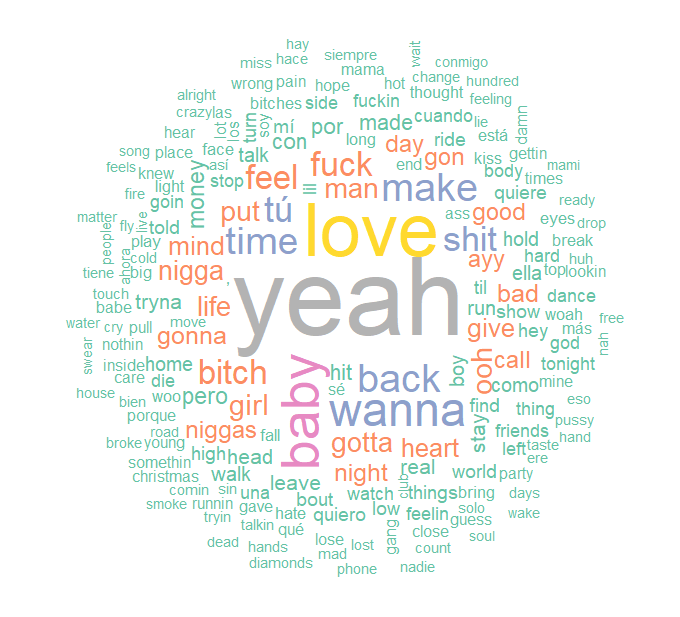
\includegraphics[width=0.5\linewidth]{Images//8_Textual//Analysis/complete_word_cloud.png}
    \caption{Wordcloud de les paraules més freqüents no traduïdes}
    \label{fig:textual_wordcloud_complete}
\end{figure}


\begin{figure}[H]
    \centering
    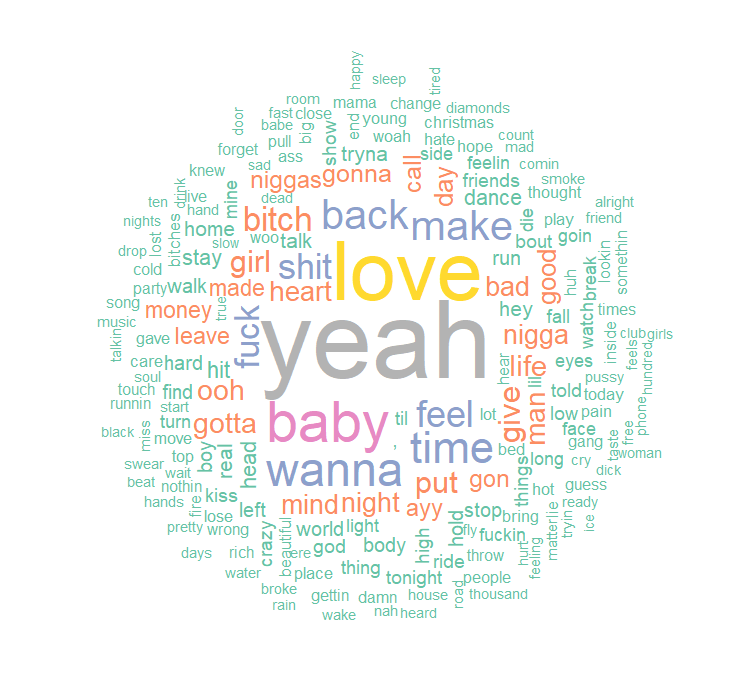
\includegraphics[width=0.5\linewidth]{Images//8_Textual//Analysis/complete_word_cloud_translated.png}
    \caption{Wordcloud de les paraules més freqüents traduïdes}
    \label{fig:textual_wordcloud_complete_translated}
\end{figure}

Les paraules que s'observen són les que apareixen més en les lletres de les cançons, i la majoria de les més freqüents estan relacionades amb un dels temes més tractats en aquestes: l'amor (\textit{love}, \textit{girl}, \textit{heart}...). Addicionalment, s'observa l'aparició de onomatopeies o interjecciosn (\textit{yeah}, \textit{ooh}, \textit{huh}, \textit{woo}...) i de paraules de \textit{slang} o argot (\textit{til}, \textit{gotta}, \textit{gonna}, \textit{gon}, \textit{tryna}...).

El sentiment de les paraules és un altre aspecte del lèxic que es pot analitzar. En aquest cas, s'ha optat per comentar els resultats del \textit{sentimental analysis} de la versió traduïda, ja que en l'altra és probable que no detecti correctament el sentiment d'algunes paraules.

Aquest anàlisi s'ha realitzat usant dos \textit{lexicons}: Bing i NRC. Per tant, hi haurà dues mesures de polaritat diferents. Es poden observar a les figures \ref{fig:textual_sentiment_bing} i \ref{fig:textual_sentiment_nrc}:

\begin{figure}[H]
\centering
    \begin{minipage}{.4\textwidth}
        \centering
        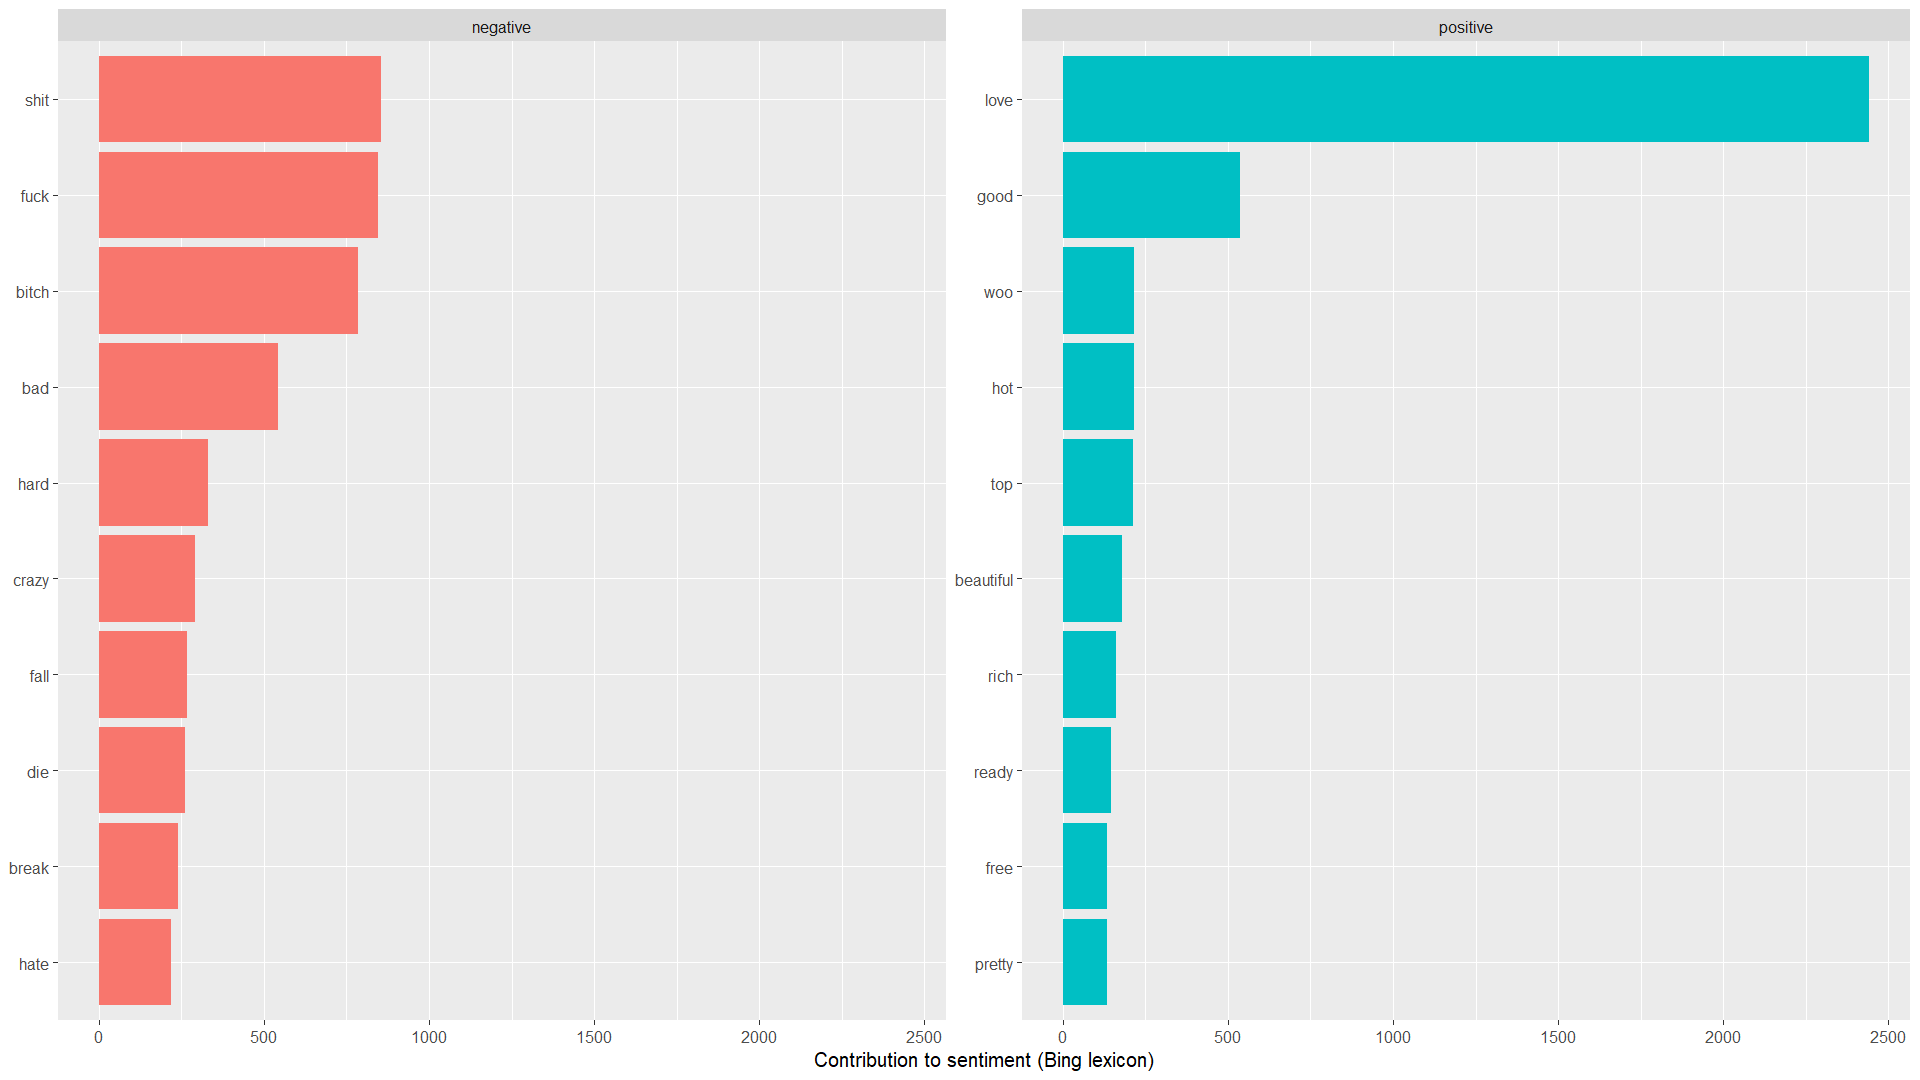
\includegraphics[width=0.95\linewidth]{Images//8_Textual//Analysis/complete_word_senti_bing.png}
        \caption{Sentimental analysis usant BING}
        \label{fig:textual_sentiment_bing}
    \end{minipage}%
    \begin{minipage}{.4\textwidth}
        \centering
        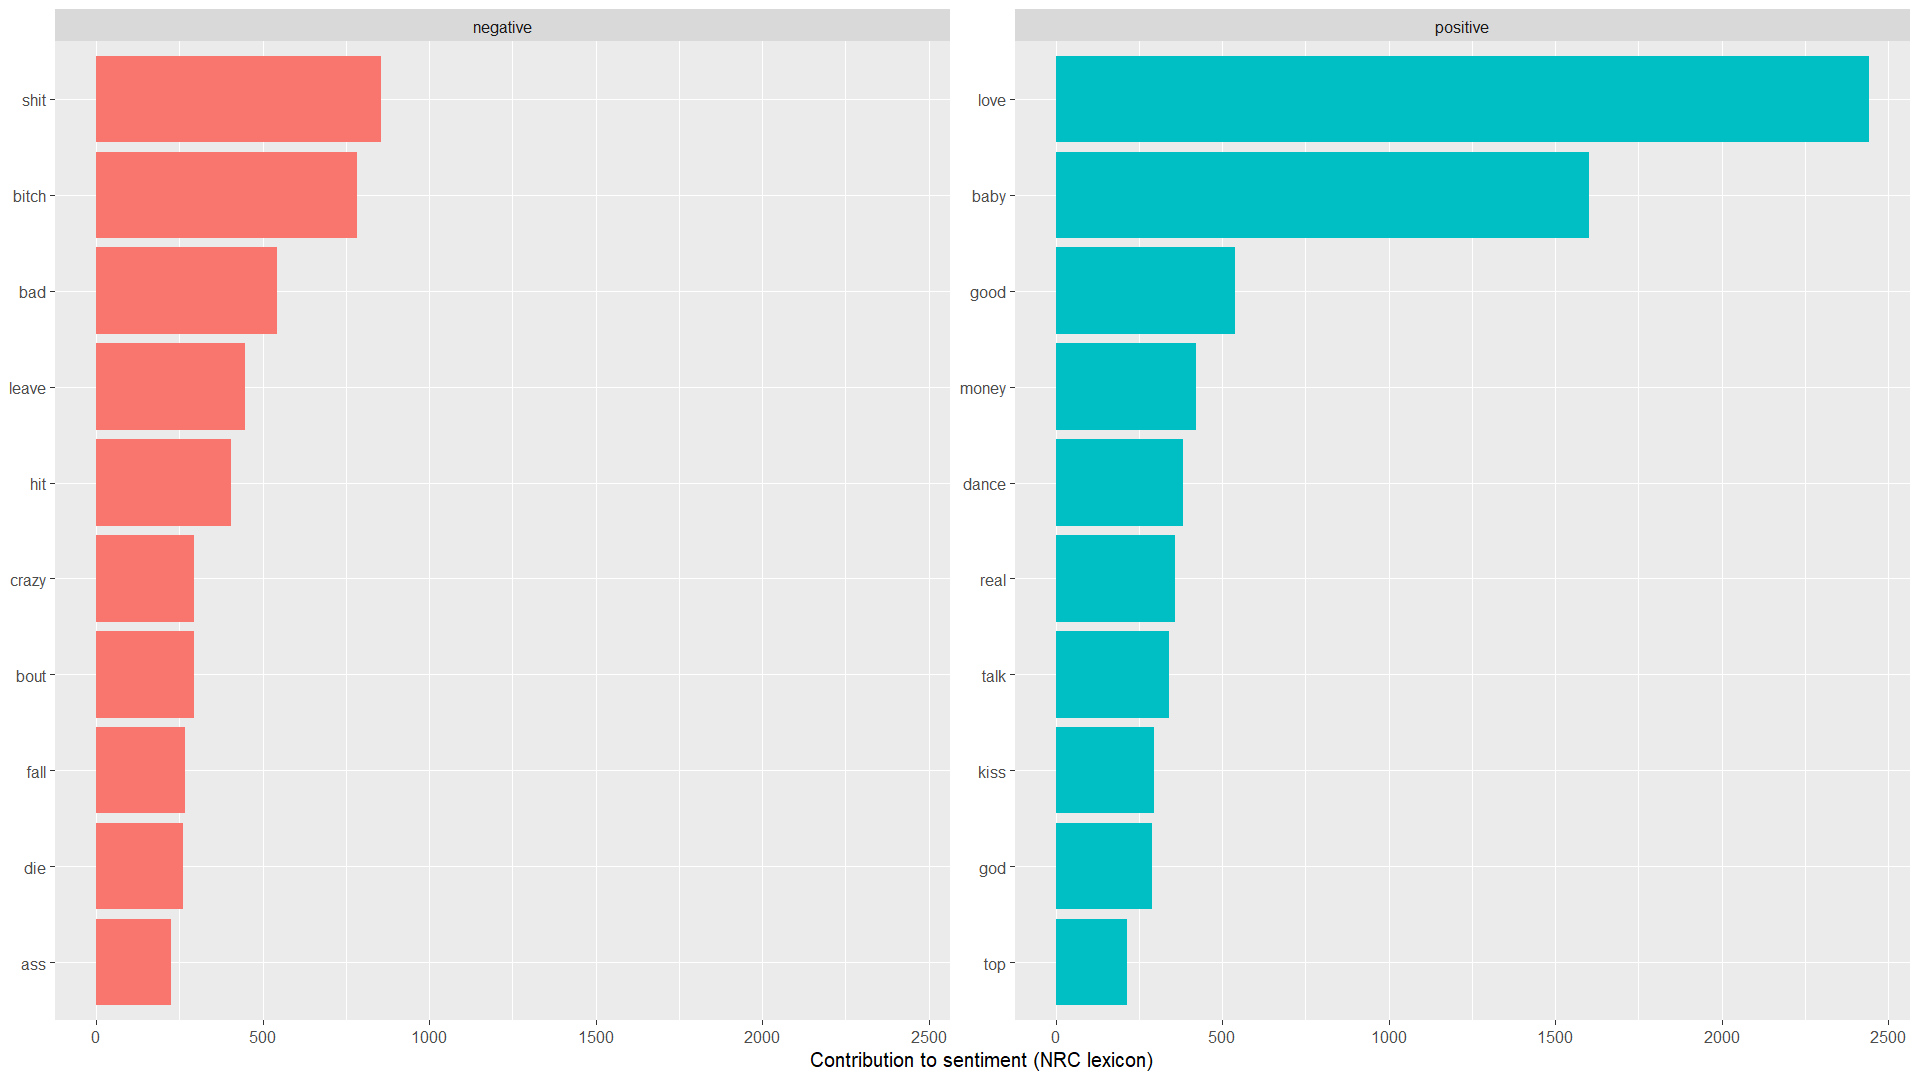
\includegraphics[width=0.95\linewidth]{Images//8_Textual//Analysis/complete_word_senti_nrc.png}
        \caption{Sentimental analysis usant BING}
        \label{fig:textual_sentiment_nrc}
    \end{minipage}%
\end{figure}

Les paraules que aporten més sentiment positiu i negatiu, en els dos casos, són \textit{love} i \textit{shit}, respectivament (la primera amb molta contribució). A continuació, el criteri provoca que apareguin paraules diferents: en bing, pels negatius tenim paraules com \textit{fuck}, \textit{bitch}, \textit{hate}... i pels positius \textit{good}, expressions com \textit{woo}, \textit{hot}, \textit{top} i adjectius. En canvi, utilitzant NRC, pels negatius per exemple desapareix \textit{fuck} i apareix \textit{ass} i \textit{bout} i pels positius \textit{baby} (amb molta importància), \textit{money}, \textit{dance}, \textit{kiss} o \textit{god}. En general, però, s'ha considerat que les sentiments de bing son més encertats, ja que l'nrc inclou algunes paraules que per si soles s'ha considerat que no serien positives ni negatives (\textit{baby}, per exemple, o \textit{bout}) i n'exclou d'altres d'importants (com \textit{fuck}). Els núvol de punts es pot observar a \ref{fig:textual_bing_wordcloud}.

\begin{figure}[H]
    \centering
    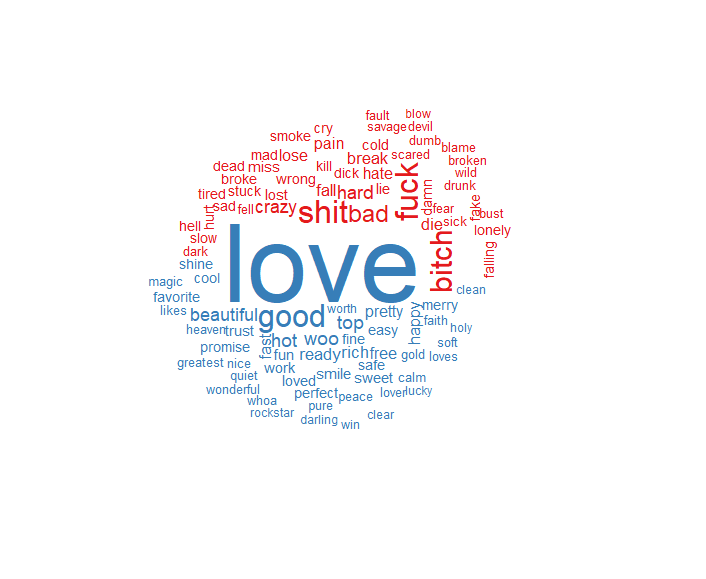
\includegraphics[width=0.7\linewidth]{Images//8_Textual//Analysis/complete_senti_cloud_bing.png}
    \caption{Núvol de punts de les paraules positives (blau) i negatives (vermell)}
    \label{fig:textual_bing_wordcloud}
\end{figure}

Aquest anàlisi de sentiments, ens ha permès observar que la majoria de paraules en les lletres de les cançons són positives (amb una gran importància de la paraula love).

Aquest anàlisi de freqüències de paraules, i de sentiments, es pot realitzar per cada cançó de manera individual (creant gràfics de barres i núvols de paraules). Addicionalment, també es pot calcular un sentiment positiu per cada track (el percentatge de positius entre la suma entre les paraules positives i les negatives). La mitjana d'aquest valor és de 0.5061, fet que indica que hi ha molt equilibri entre cançons positives i negatives (i per tant, sembla ser que usar paraules positives o negatives no influeix per tal d'estar al top 40 de Spotify). Amb aquesta nova columna, es poden realitzar els plots de les figures \ref{fig:textual_sentiment_genre} i \ref{fig:textual_sentiment_explicit}.

\begin{figure}[H]
    \centering
    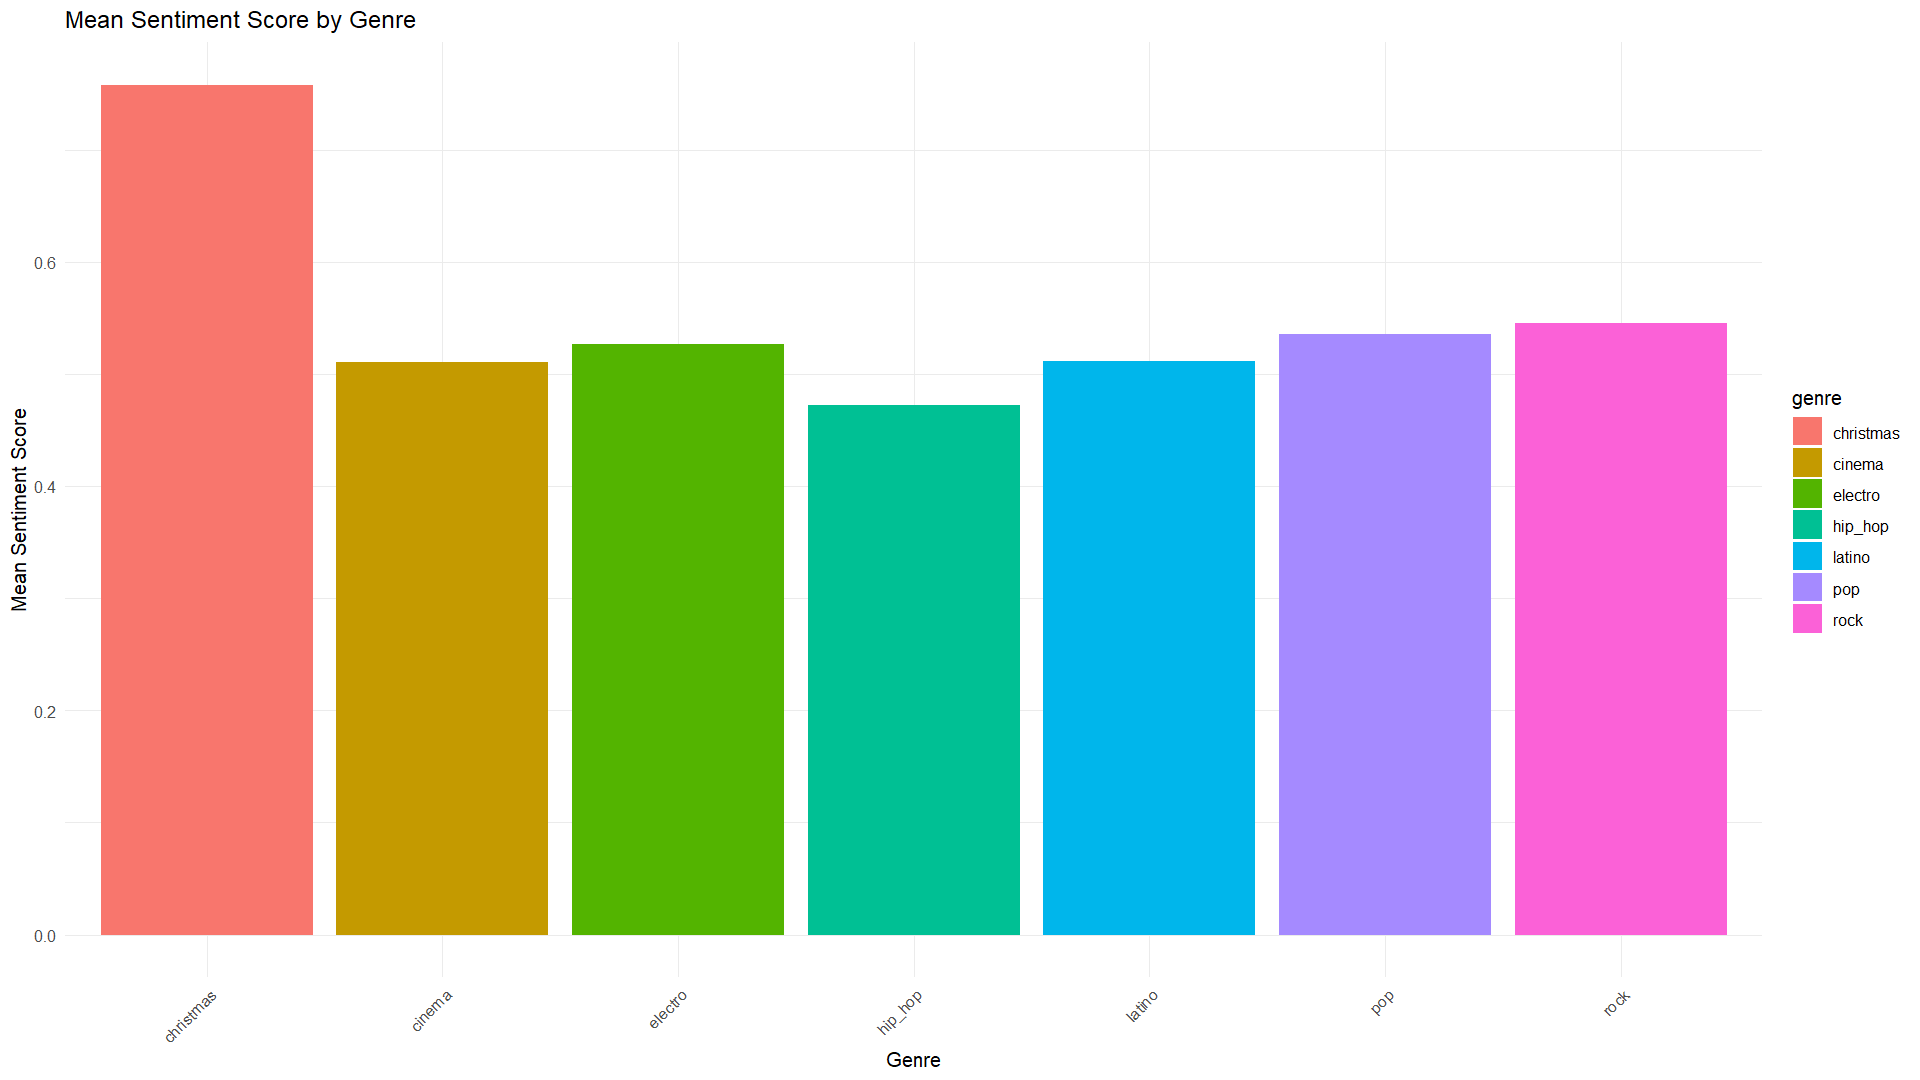
\includegraphics[width=0.7\linewidth]{Images//8_Textual//Analysis/mean_sentiment_genre.png}
    \caption{Mitjana de sentiment positiu per gènere}
    \label{fig:textual_sentiment_genre}
\end{figure}

\begin{figure}[H]
    \centering
    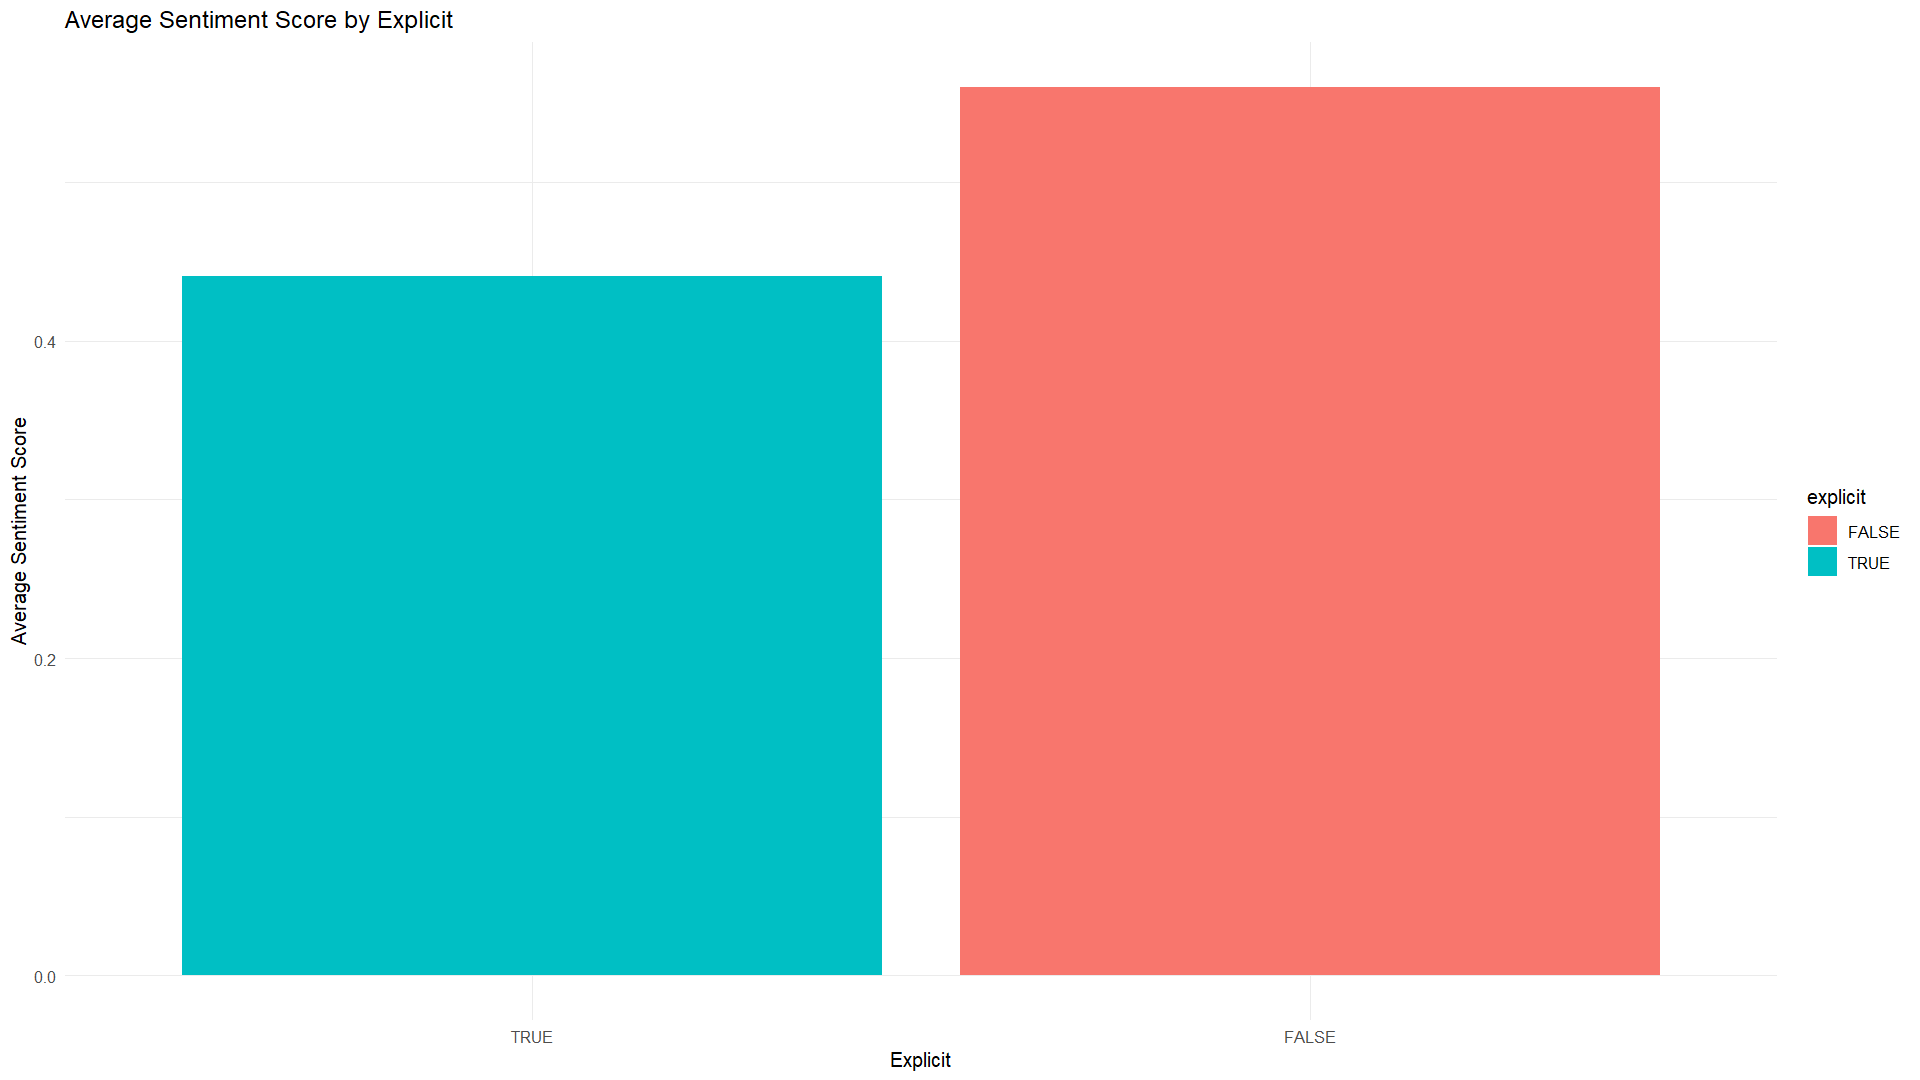
\includegraphics[width=0.7\linewidth]{Images//8_Textual//Analysis/mean_sentiment_explicit.png}
    \caption{Mitjana de sentiment positiu segons explicit}
    \label{fig:textual_sentiment_explicit}
\end{figure}

Segons els gèneres musicals, destaca sobretot \textit{christmas}, un gènere molt positiu, mentre que \textit{hip hop} és el menys positiu de tots. Respecte a explicit, observem com el fet que una cançó sigui explícita també indica que utilitzi paraules menys positives (la majoria de paraules malsonants es consideren negatives).

\subsubsection{Anàlisi d'emocions}
A més de l'anàlisi de positivitat o negativitat, s'ha realitzat també una anàlisi respecte altres emocions. En concret: \textit{anger}, \textit{anticipation}, \textit{disgust}, \textit{fear}, \textit{joy}, \textit{sadness}, \textit{surprise} i \textit{trust}. Observem el núvol de punts \ref{fig:textual_emotions_cloud} i les freqüències \ref{fig:textual_emotions_bar}.

\begin{figure}[H]
    \centering
    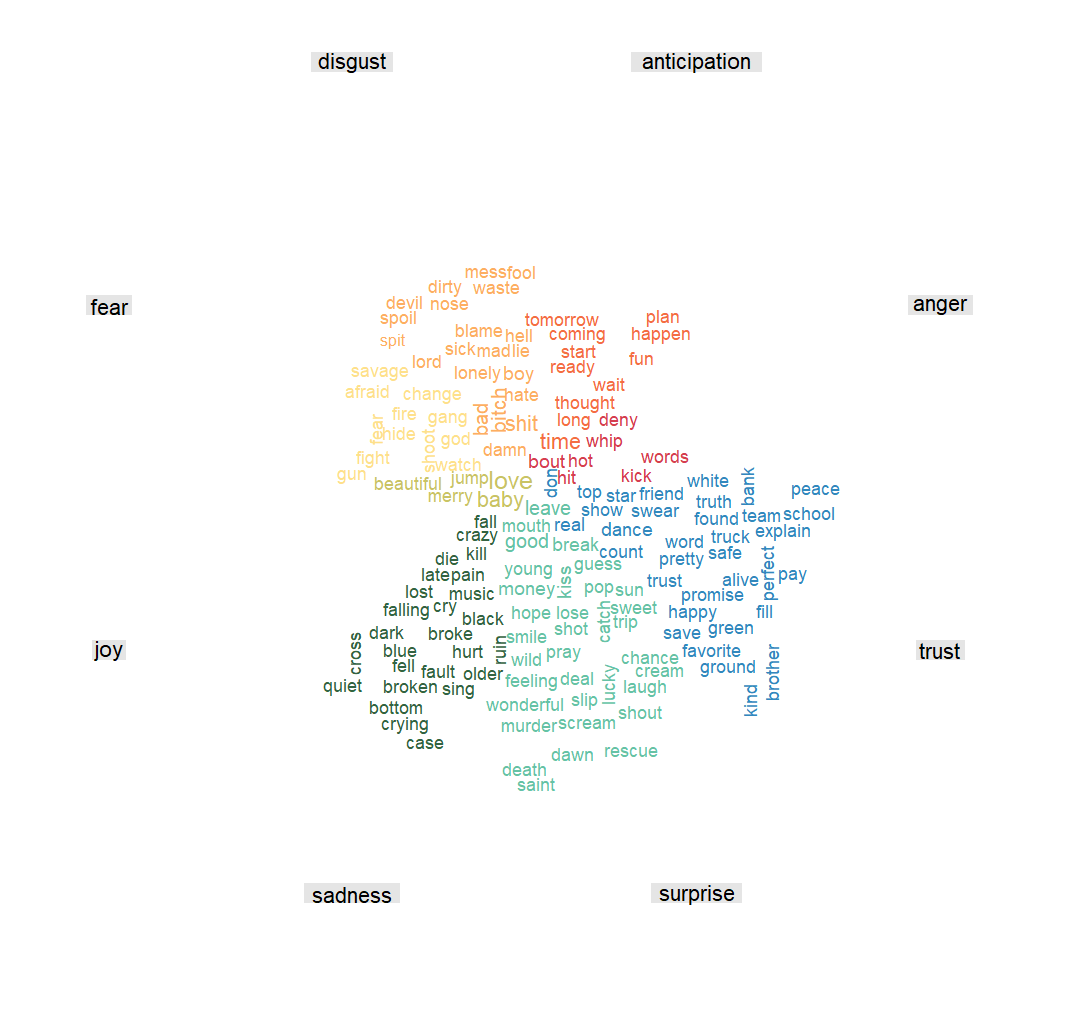
\includegraphics[width=0.7\linewidth]{Images//8_Textual//Analysis/emotions_cloud.png}
    \caption{Núvol de punts de les emocions}
    \label{fig:textual_emotions_cloud}
\end{figure}

\begin{figure}[H]
    \centering
    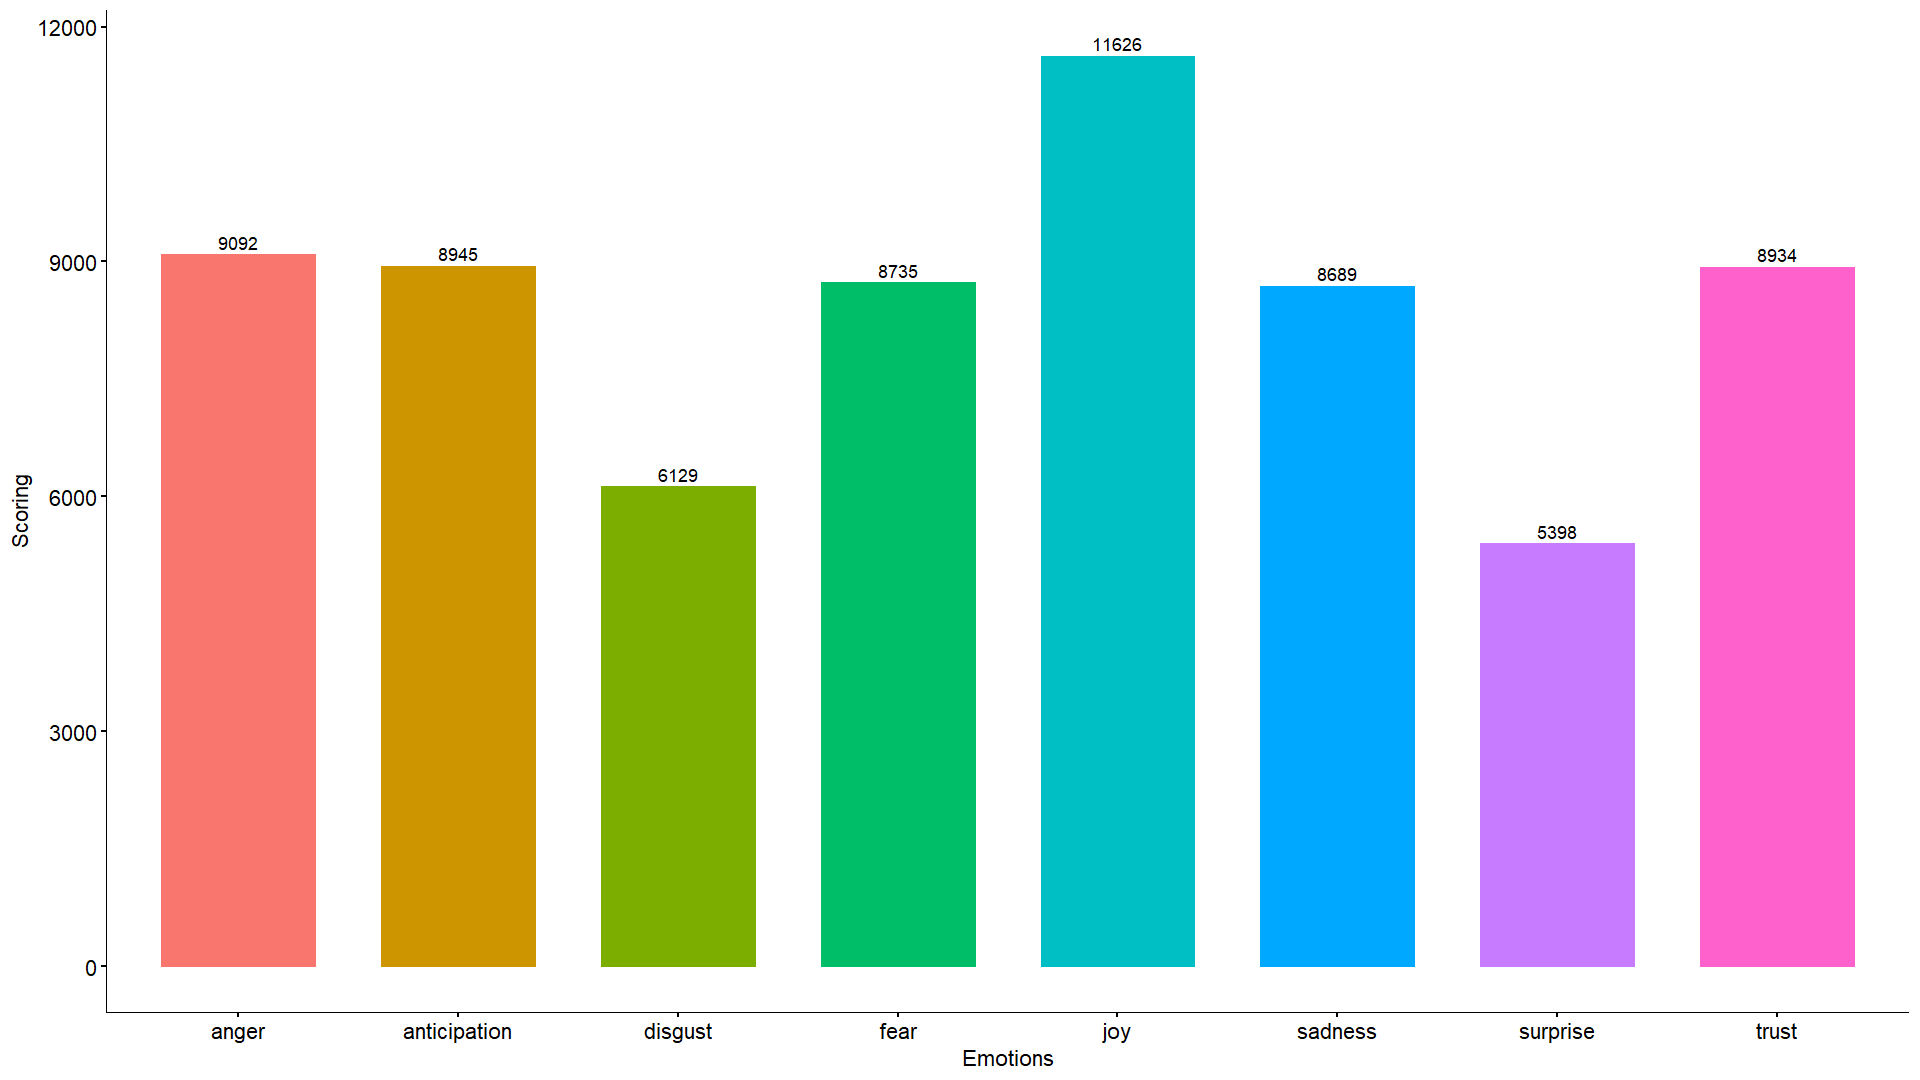
\includegraphics[width=0.7\linewidth]{Images//8_Textual//Analysis/emotions_scoring.png}
    \caption{Gràfic de barres de les emocions}
    \label{fig:textual_emotions_bar}
\end{figure}

Observem com la majoria de paraules del text expressen alegria (\textit{joy}). Les dues emocions que menys apareixen en les nostres paraules son disgust i surprise. Addicionalment, igual que en l'apartat anterior, s'ha passat de la informació sobre cada paraula a la informació per track. Amb això, podem observar altre cop la distribució segons el gènere \ref{fig:textual_emotions_genre}.

\begin{figure}[H]
    \centering
    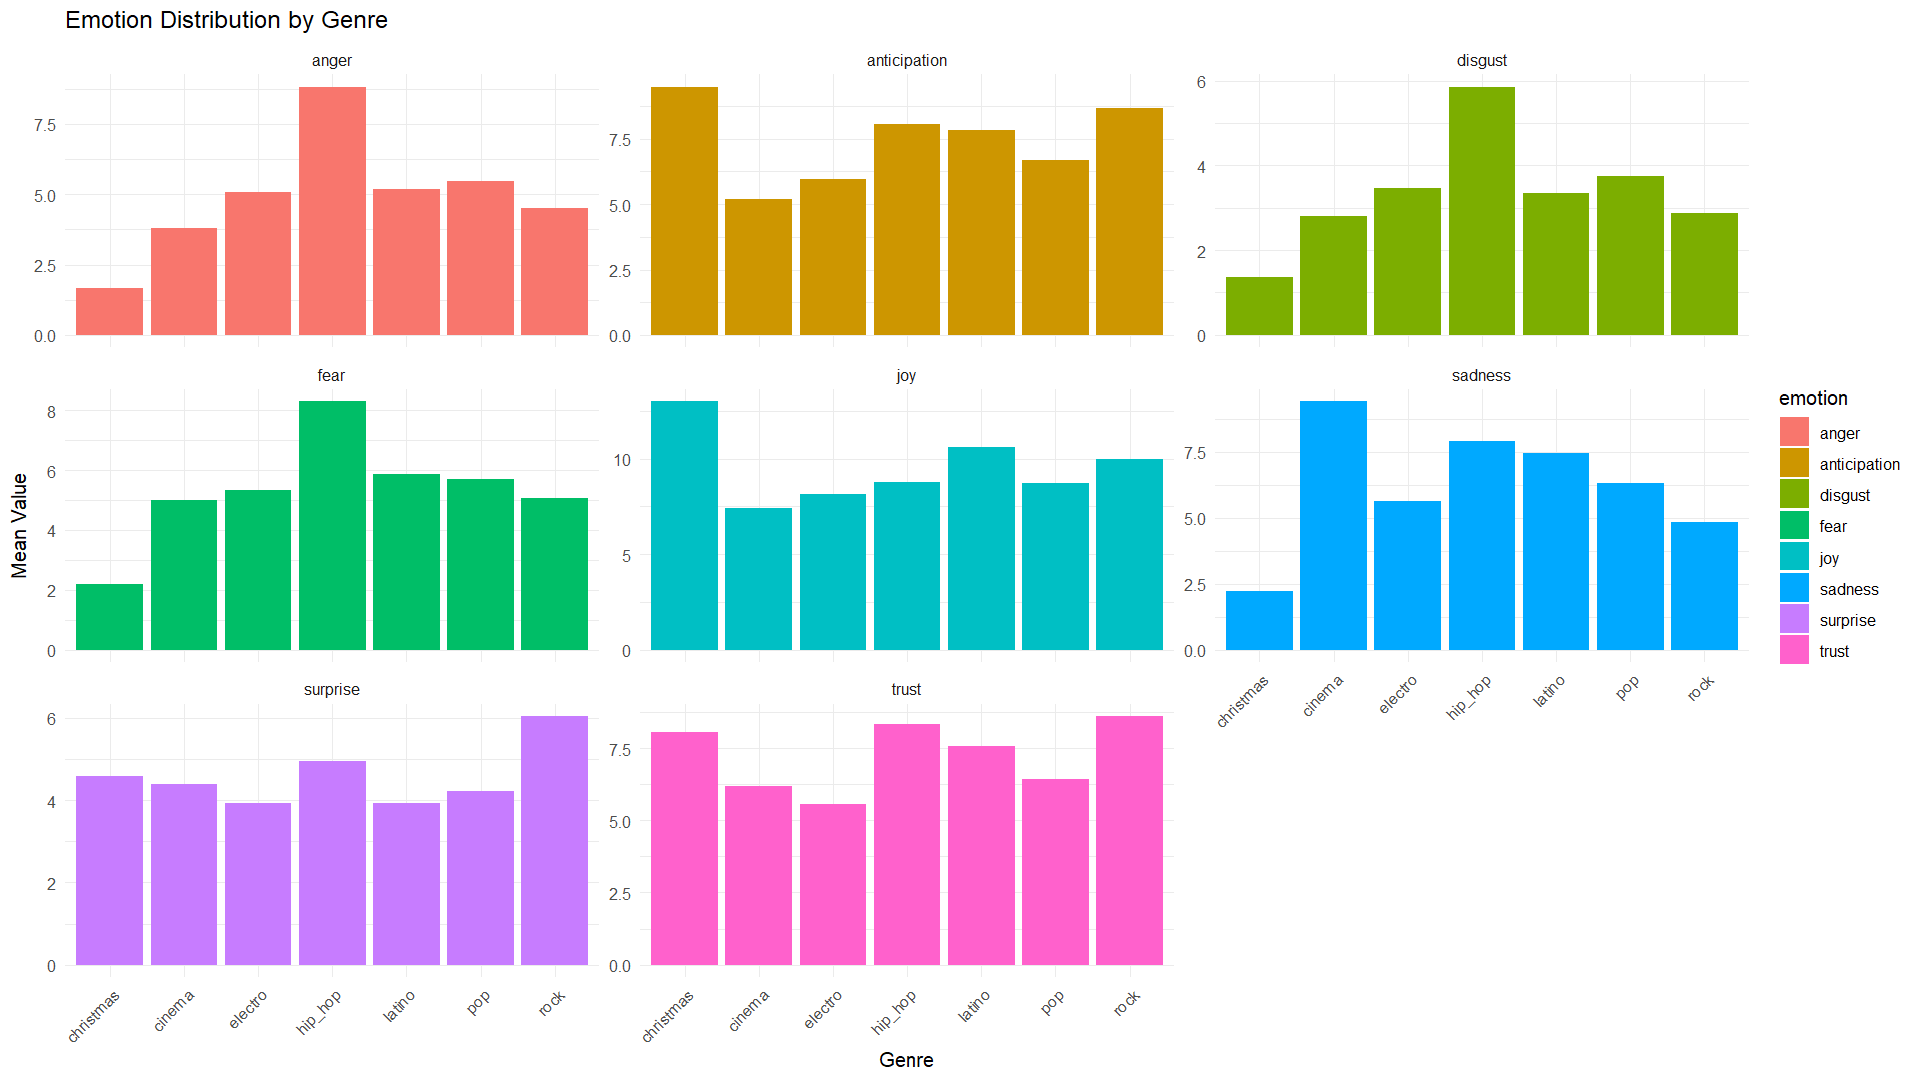
\includegraphics[width=0.7\linewidth]{Images//8_Textual//Analysis/mean_emotions_genre.png}
    \caption{Emocions en funció del gènere}
    \label{fig:textual_emotions_genre}
\end{figure}

S'observa com \textit{christmas} té molta alegria i anticipació (i poquíssimes paraules tristes). En canvi, també es pot veure com hip hop té molt d'odi (\textit{anger}), por i disgust. La resta de gèneres no es diferencien gaire del pop (tampoc tenen gaires cançons), com a molt en la tristesa on cinema, hip hop i latino són els que més utilitzen paraules tristes.

També s'ha volgut, però, observar si hi havia alguna tendència temporal relacionada amb les emocions de les paraules que utilitzen les cançons. Per detectar-ho, s'ha realitzat un plot de sèries temporals amb el valor mig de cada emoció mensualment (entre 2017 i 2021) \ref{fig:textual_emotions_time_series}.

\begin{figure}[H]
    \centering
    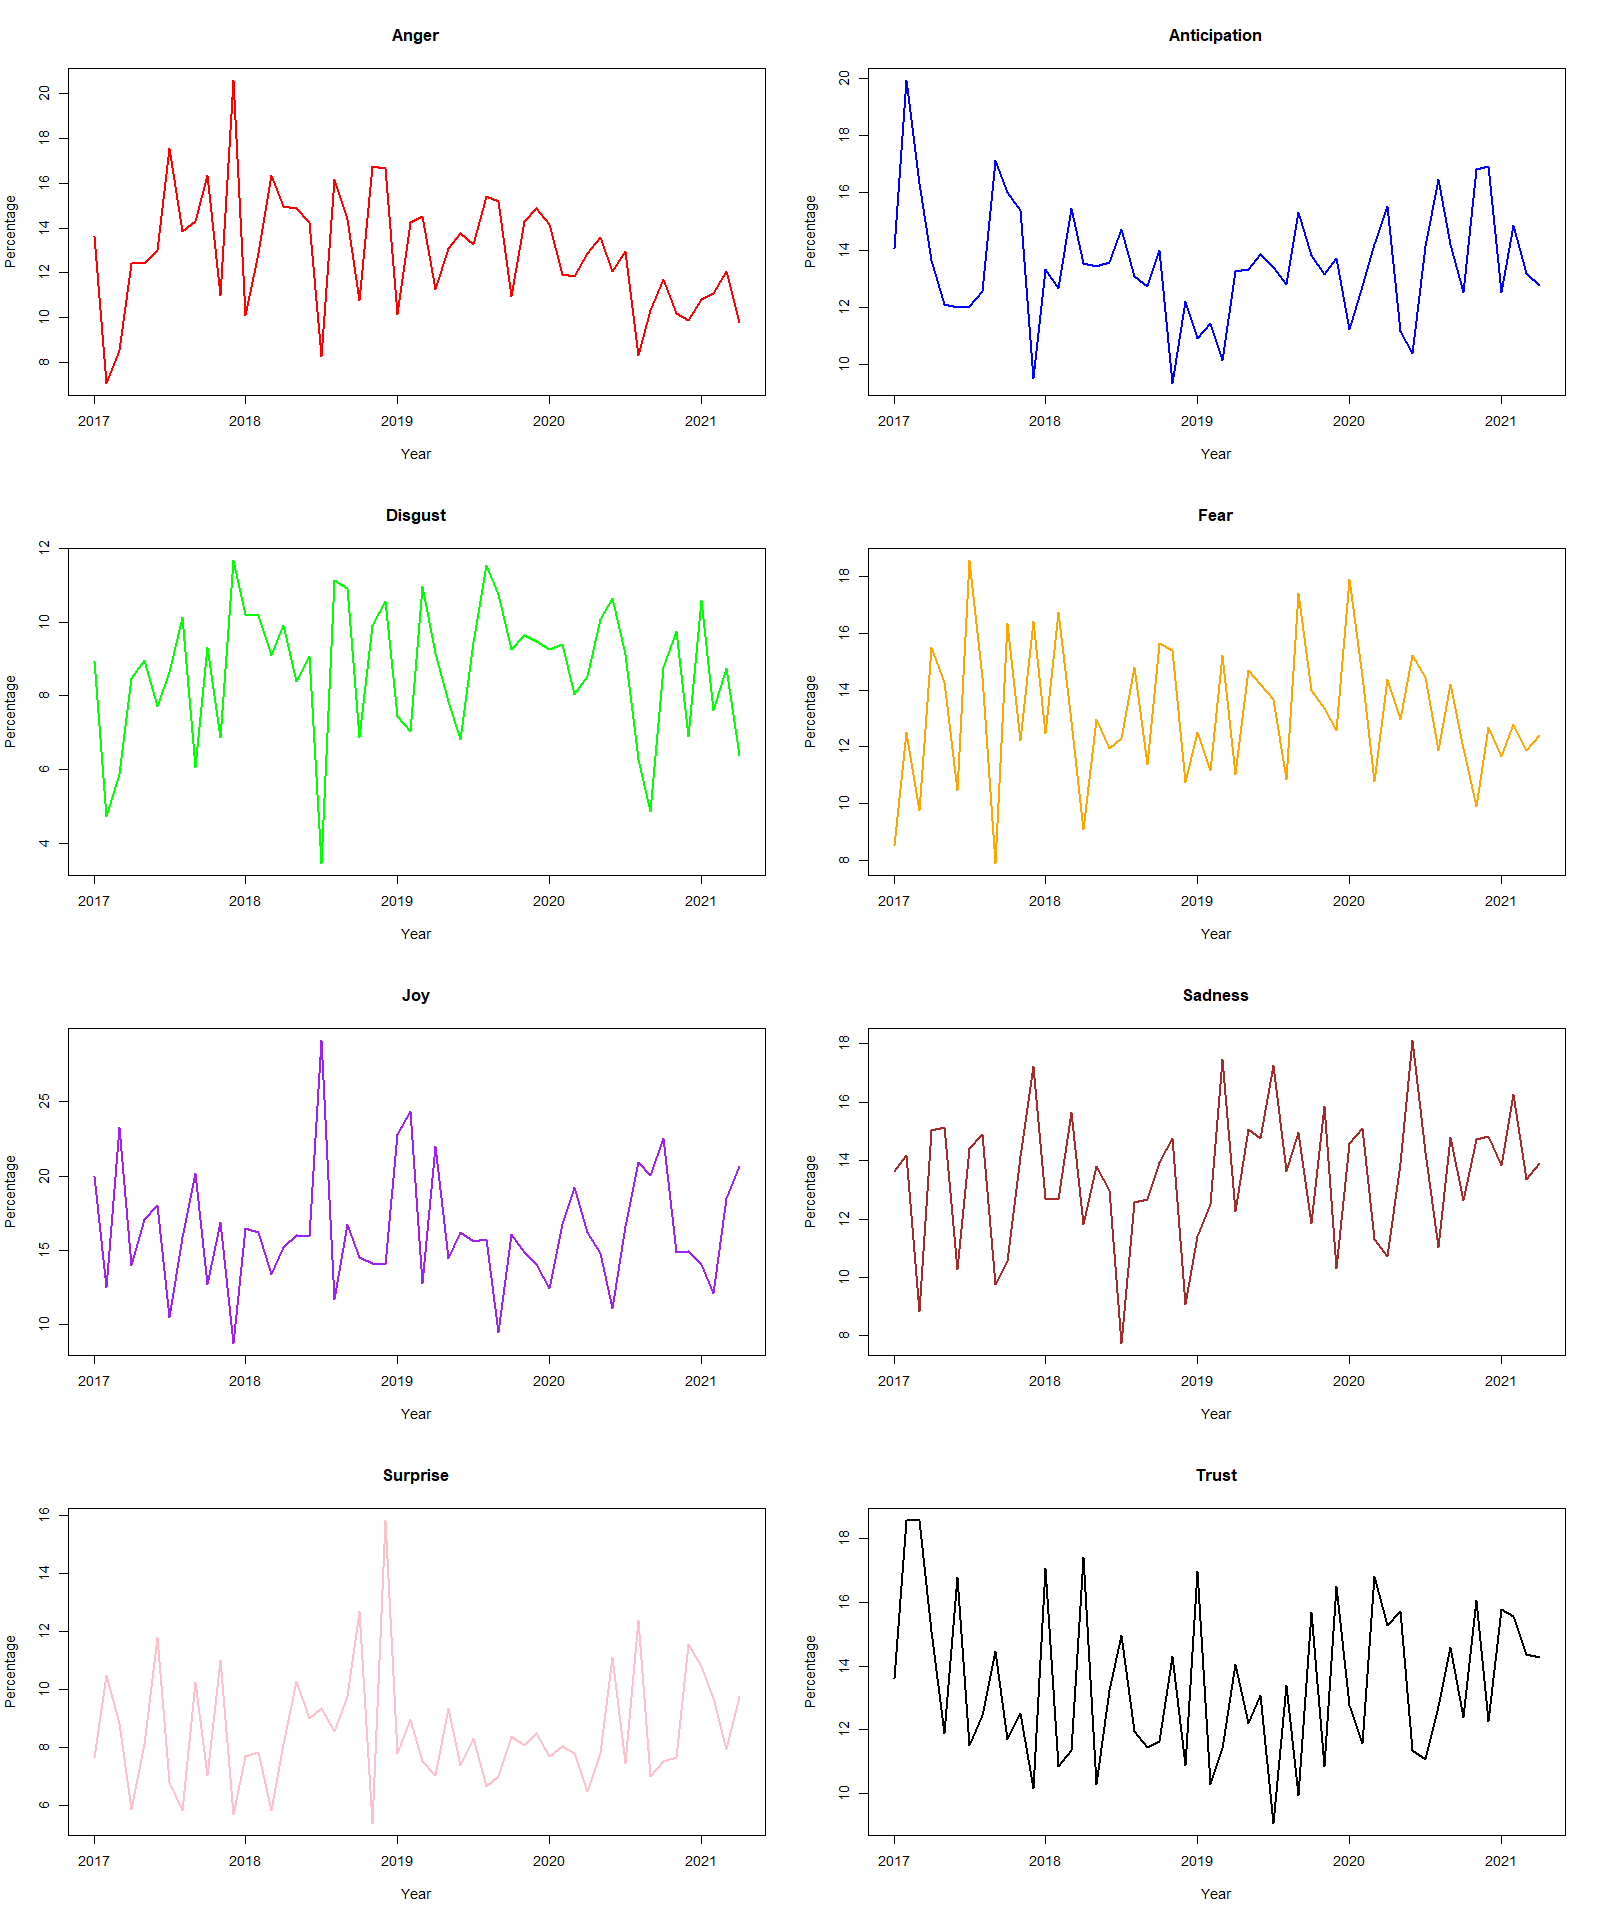
\includegraphics[width=0.7\linewidth]{Images//8_Textual//Analysis/all_time_series.png}
    \caption{Sèrie temporal de les emocions}
    \label{fig:textual_emotions_time_series}
\end{figure}

No s'observen gaires tendències molt marcades, tot i que sí que és veritat que l'odi (\textit{anger}) sembla ser que té tendència a disminuïr, (i sadness a augmentar). Sorprenentment, tampoc s'observa cap canvi en la quarentena (cal recordar que aquestes dades són d'entre 2017 i 2021, o sigui quan va començar la COVID).

\subsection{Anàlisi de correspondències}
Després de realitzar aquest primer anàlisi inicial, s'ha realitzat un anàlisi de correspondències (CA) i un CA-GALT amb aquestes mateixes dades.

En l'anàlisi de correspondències simple, observem que la variància explicada per les dues primeres dimensions és molt poca (0.8\% cada dimensió). Es poden visualitzar tant els documents \ref{fig:textual_ca_documents} com les paraules \ref{fig:textual_ca_words} en aquest espai.

\begin{figure}[H]
\centering
    \begin{minipage}{.4\textwidth}
        \centering
        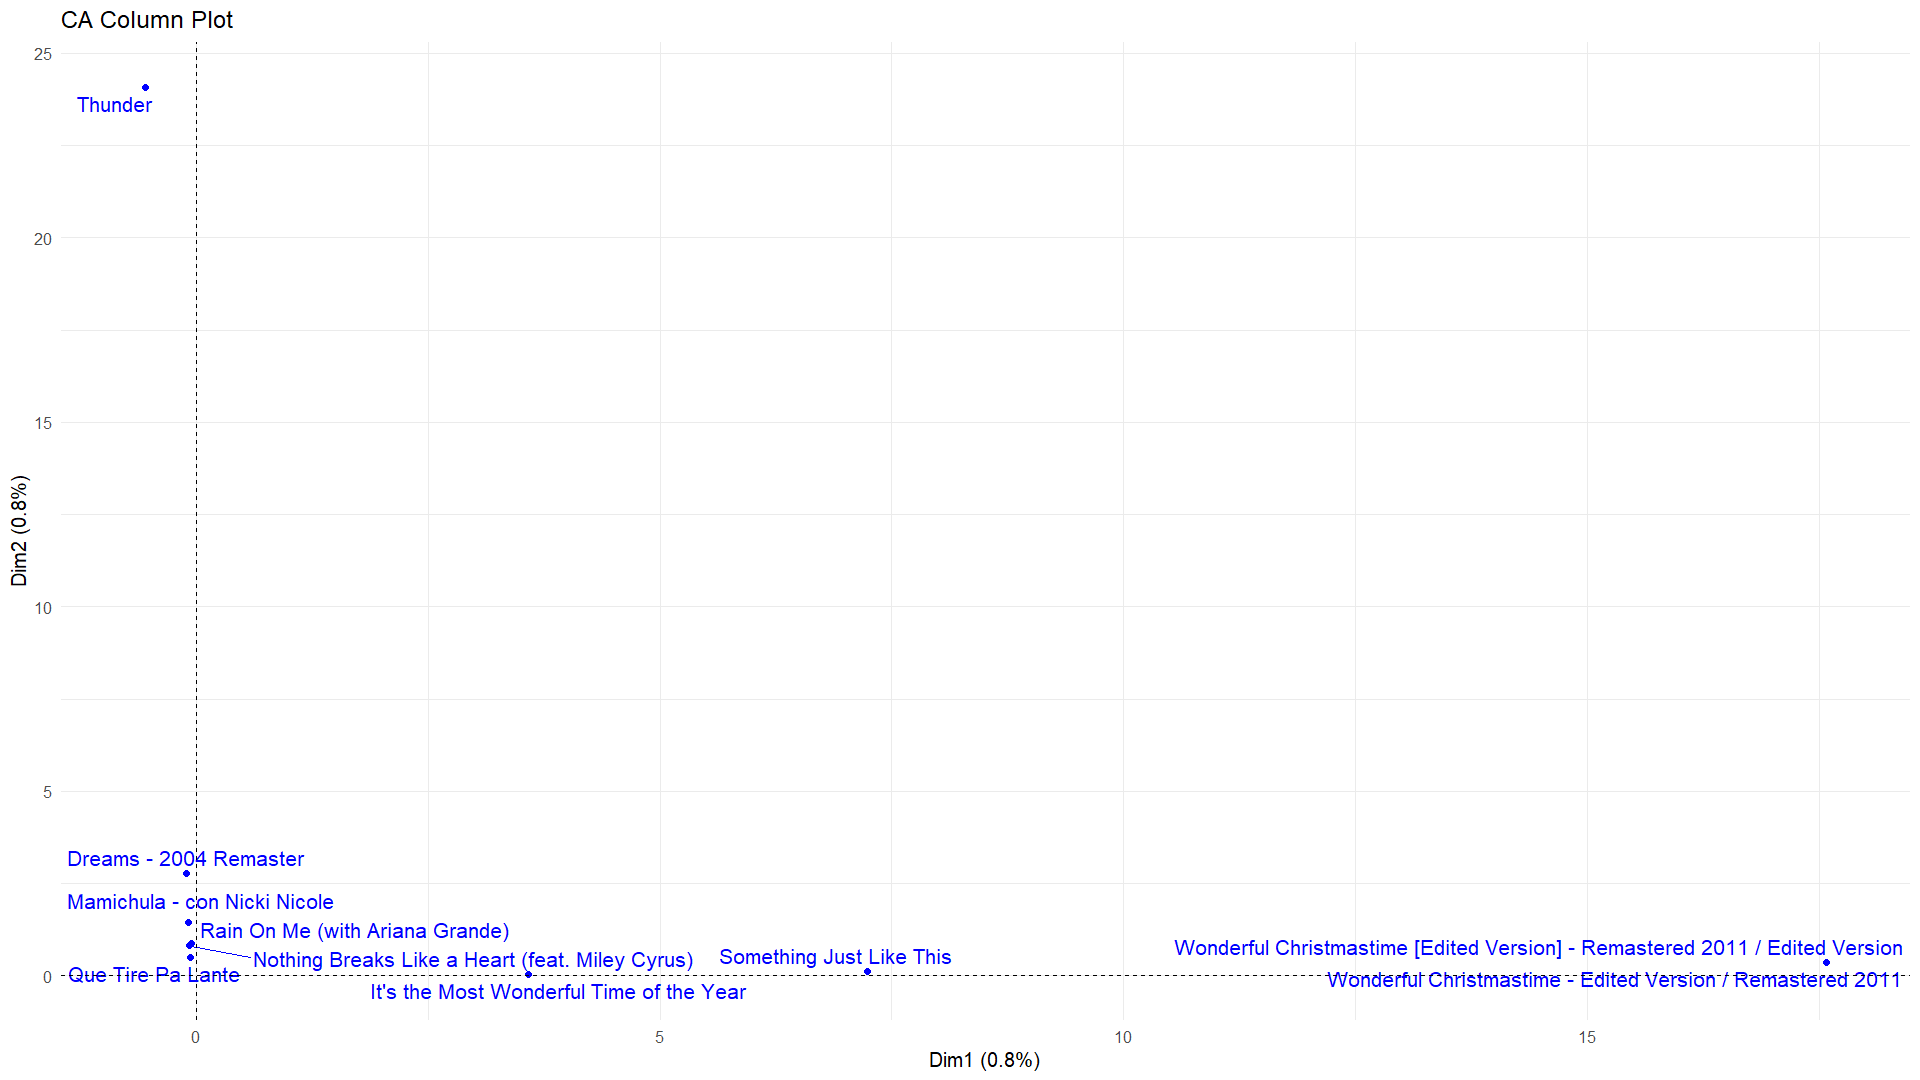
\includegraphics[width=0.95\linewidth]{Images//8_Textual//Analysis/ca_documents_12.png}
        \caption{Documents (10 més significants) visualitzats en l'anàlisi de correspondències simple}
        \label{fig:textual_ca_documents}
    \end{minipage}%
    \begin{minipage}{.4\textwidth}
        \centering
        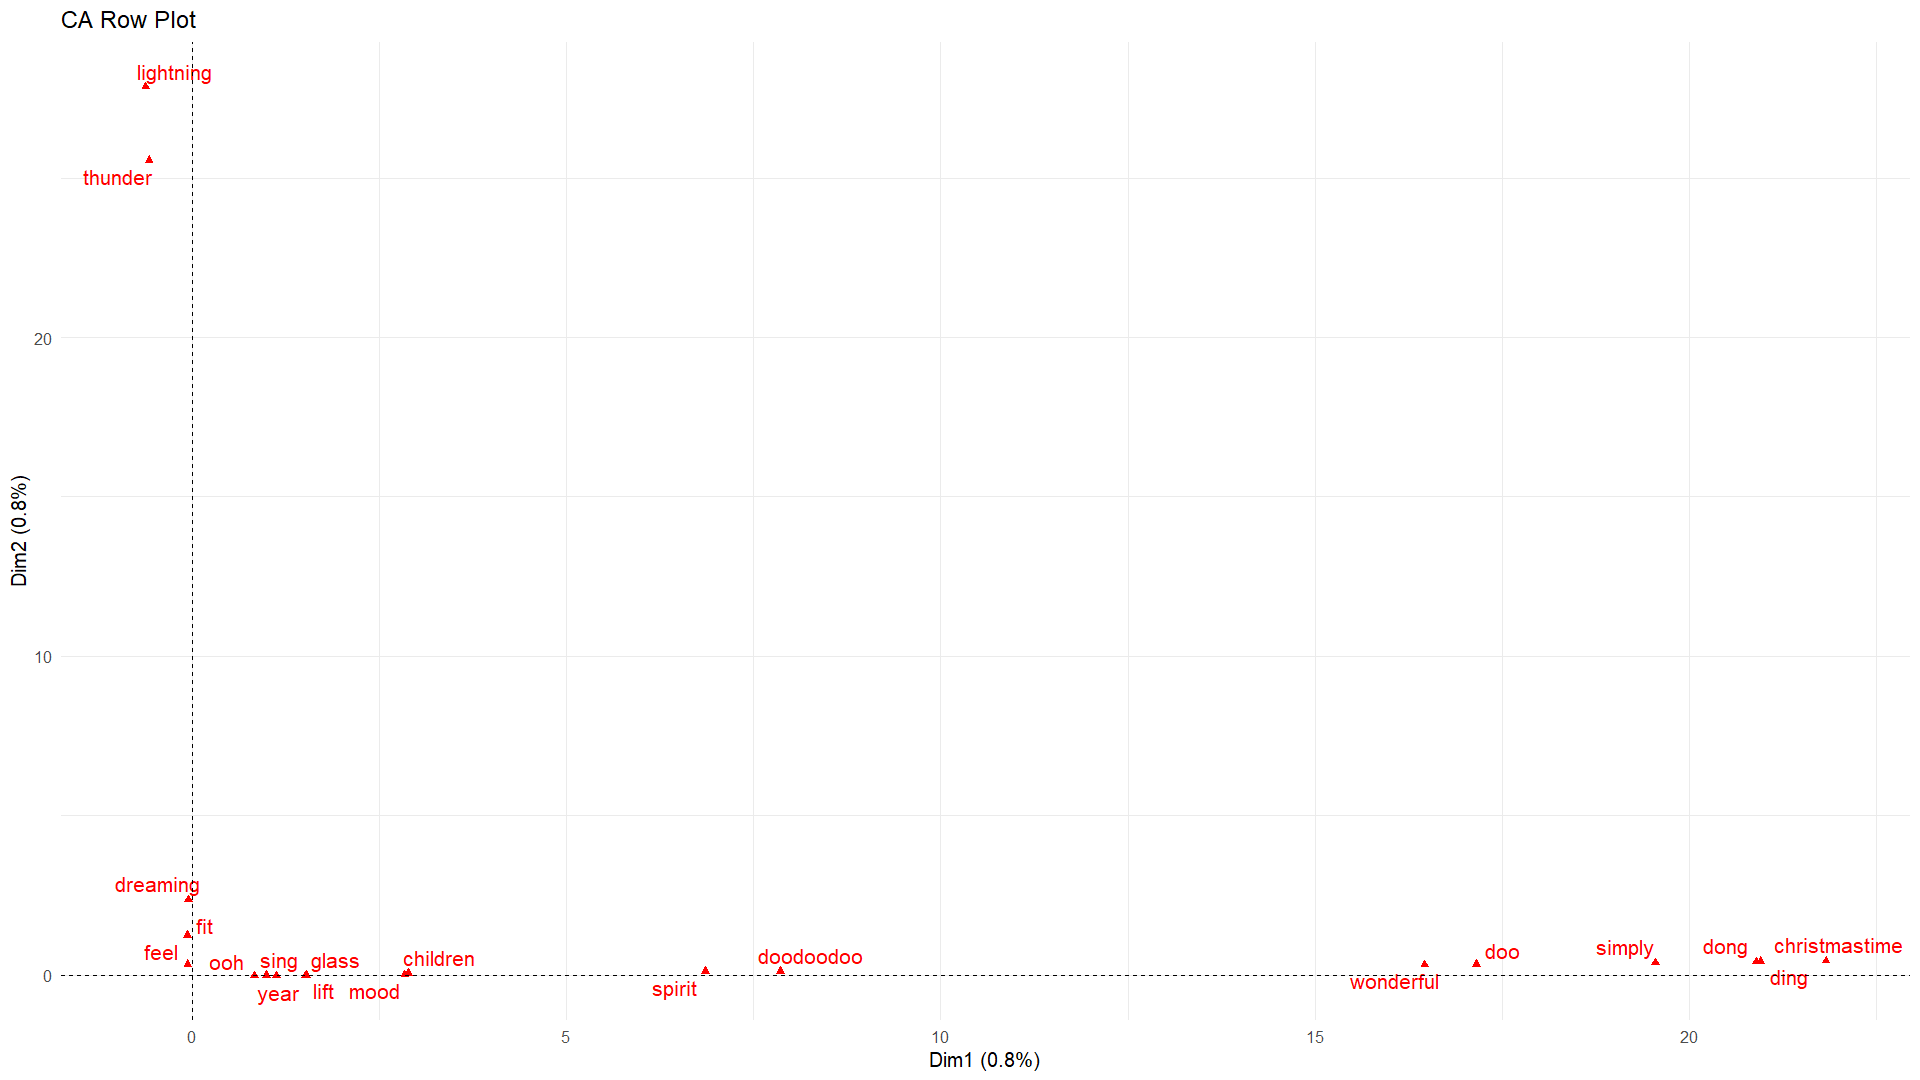
\includegraphics[width=0.95\linewidth]{Images//8_Textual//Analysis/ca_words_12.png}
        \caption{Paraules (10 més significants) visualitzades en l'anàlisi de correspondències simple}
        \label{fig:textual_ca_words}
    \end{minipage}%
\end{figure}

Com es pot apreciar, els punts es distribueixen totalment entorn als eixos, o a prop de l'origen. De fet, s'observa com és pràcticament tant sols un document el que identifica un eix (en el cas del primer, \textit{Wonderful Christmastime}\ref{fig:textual_ca_contrib_docs_1}.

\begin{figure}[H]
    \centering
    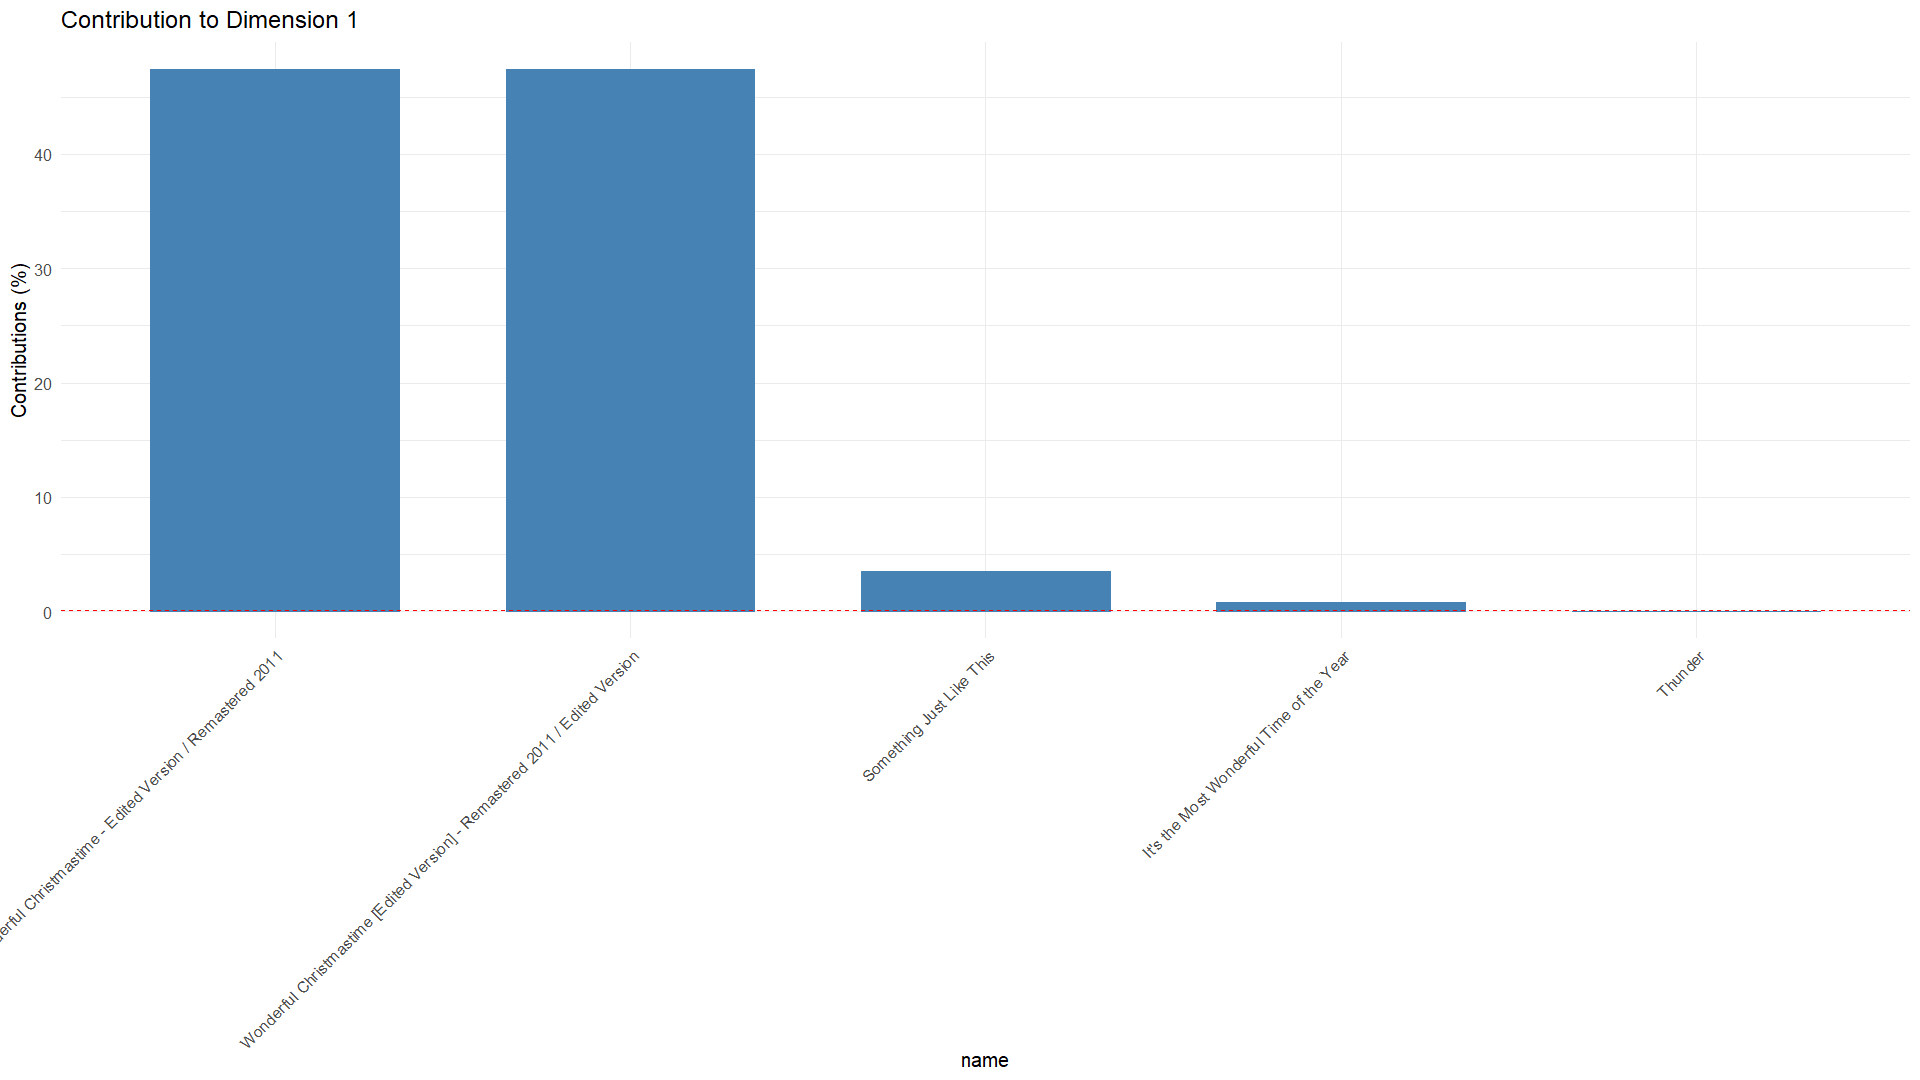
\includegraphics[width=0.7\linewidth]{Images//8_Textual//Analysis/1_dimension_docs.png}
    \caption{Contribució dels documents a la primera dimensió}
    \label{fig:textual_ca_contrib_docs_1}
\end{figure}

Aquest anàlisi, per tant, realment no ens proporciona informació gaire útil, ja que la variància explicada és molt insigificant, i a més les dimensions venen tan sols determinades per un document. Per intentar solucionar aquest problema, s'ha realitzat el CA-GALT, és a dir: aquest mateix anàlisi de correspondències, però afegint també algunes variables (en aquest cas numèriques: \textit{danceability}, \textit{streams}, \textit{track\_popularity}, \textit{energy}, \textit{acousticness}, \textit{liveness}, \textit{valence} i \textit{duration}).

Amb aquestes variables, la variància explicada en les primeres dimensions augmenta de forma molt considerable, passant a un 17.97\% i 14.74\% en les dues primeres dimensions. Podem observar, en aquest espai, els individus (\textit{tracks}, cançons), les paraules (frequencies) i aquestes variables qualitatives:

\begin{figure}[H]
    \centering
    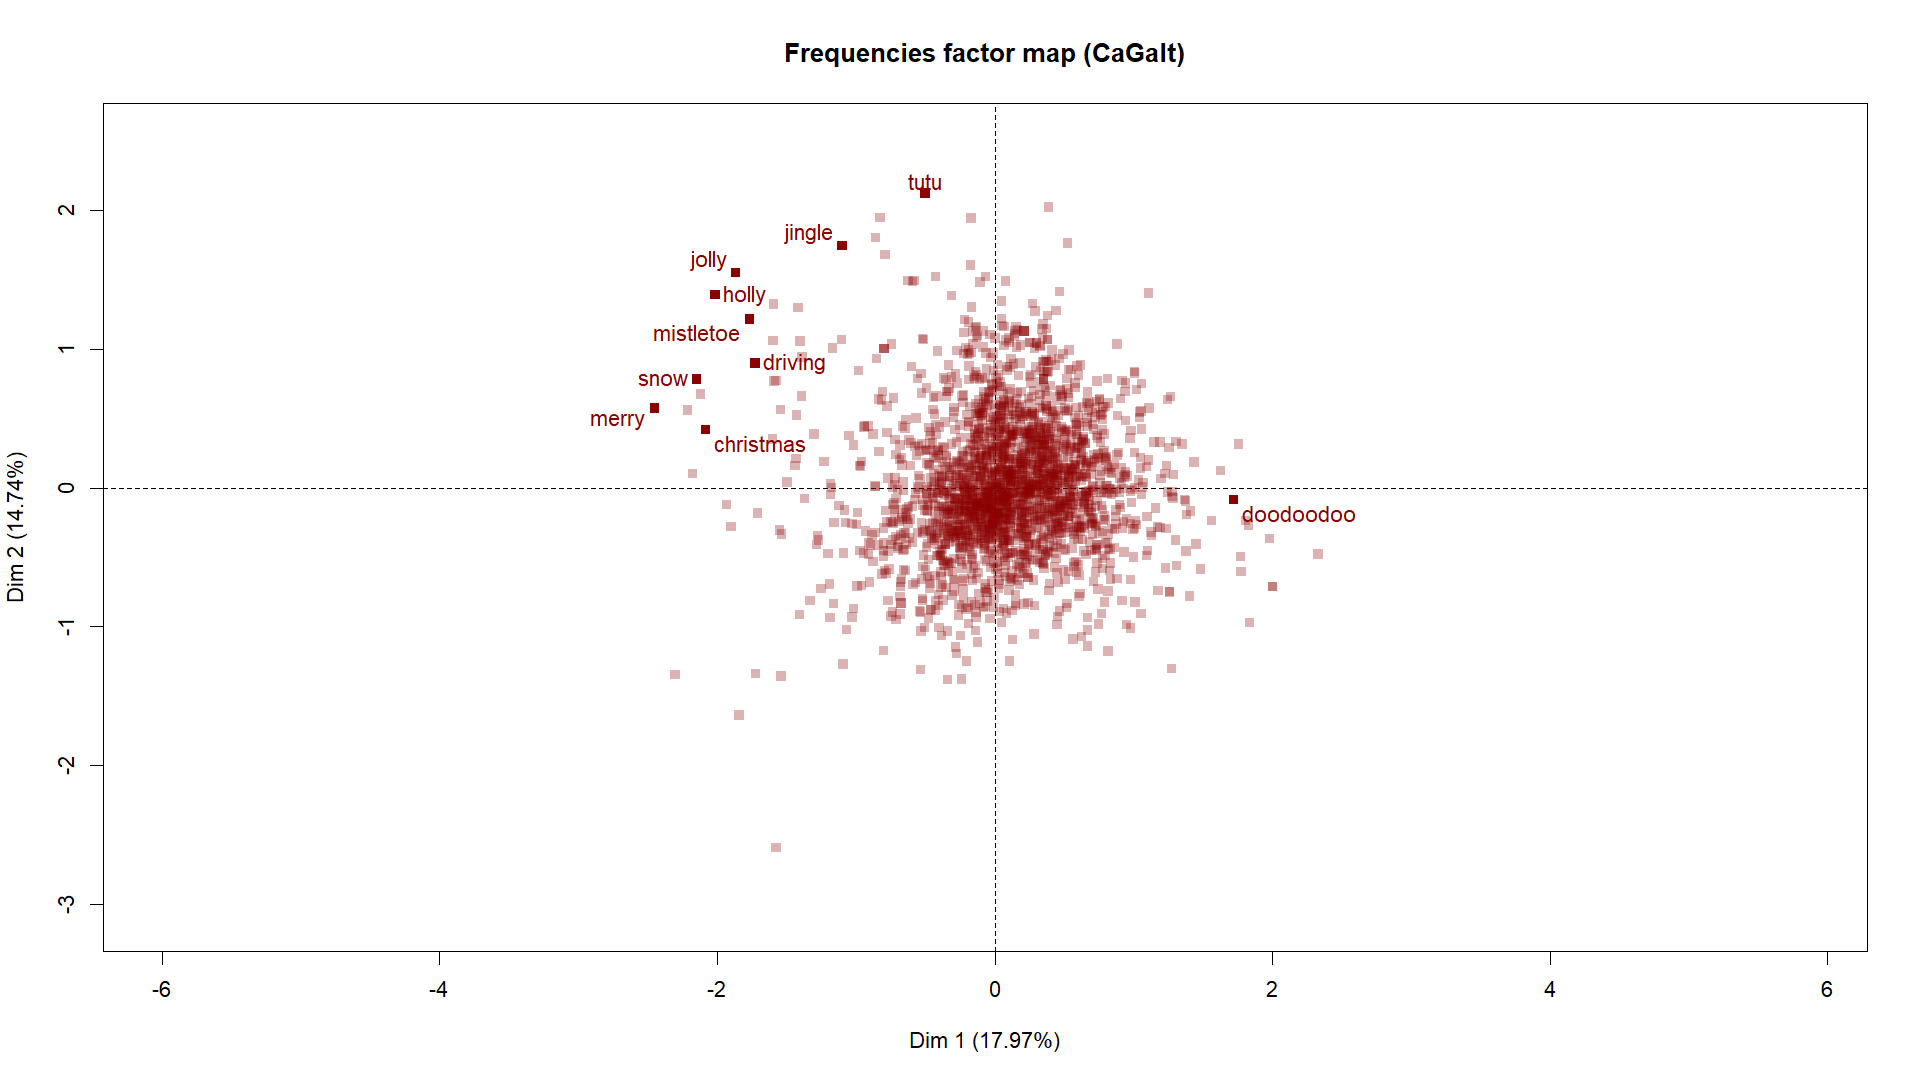
\includegraphics[width=0.7\linewidth]{Images//8_Textual//Analysis/cagalt_words_12.png}
    \caption{Paraules en CA-GALT amb numèriques en les dues primeres dimensions}
    \label{fig:textual_cagaltnum_words12}
\end{figure}

\begin{figure}[H]
    \centering
    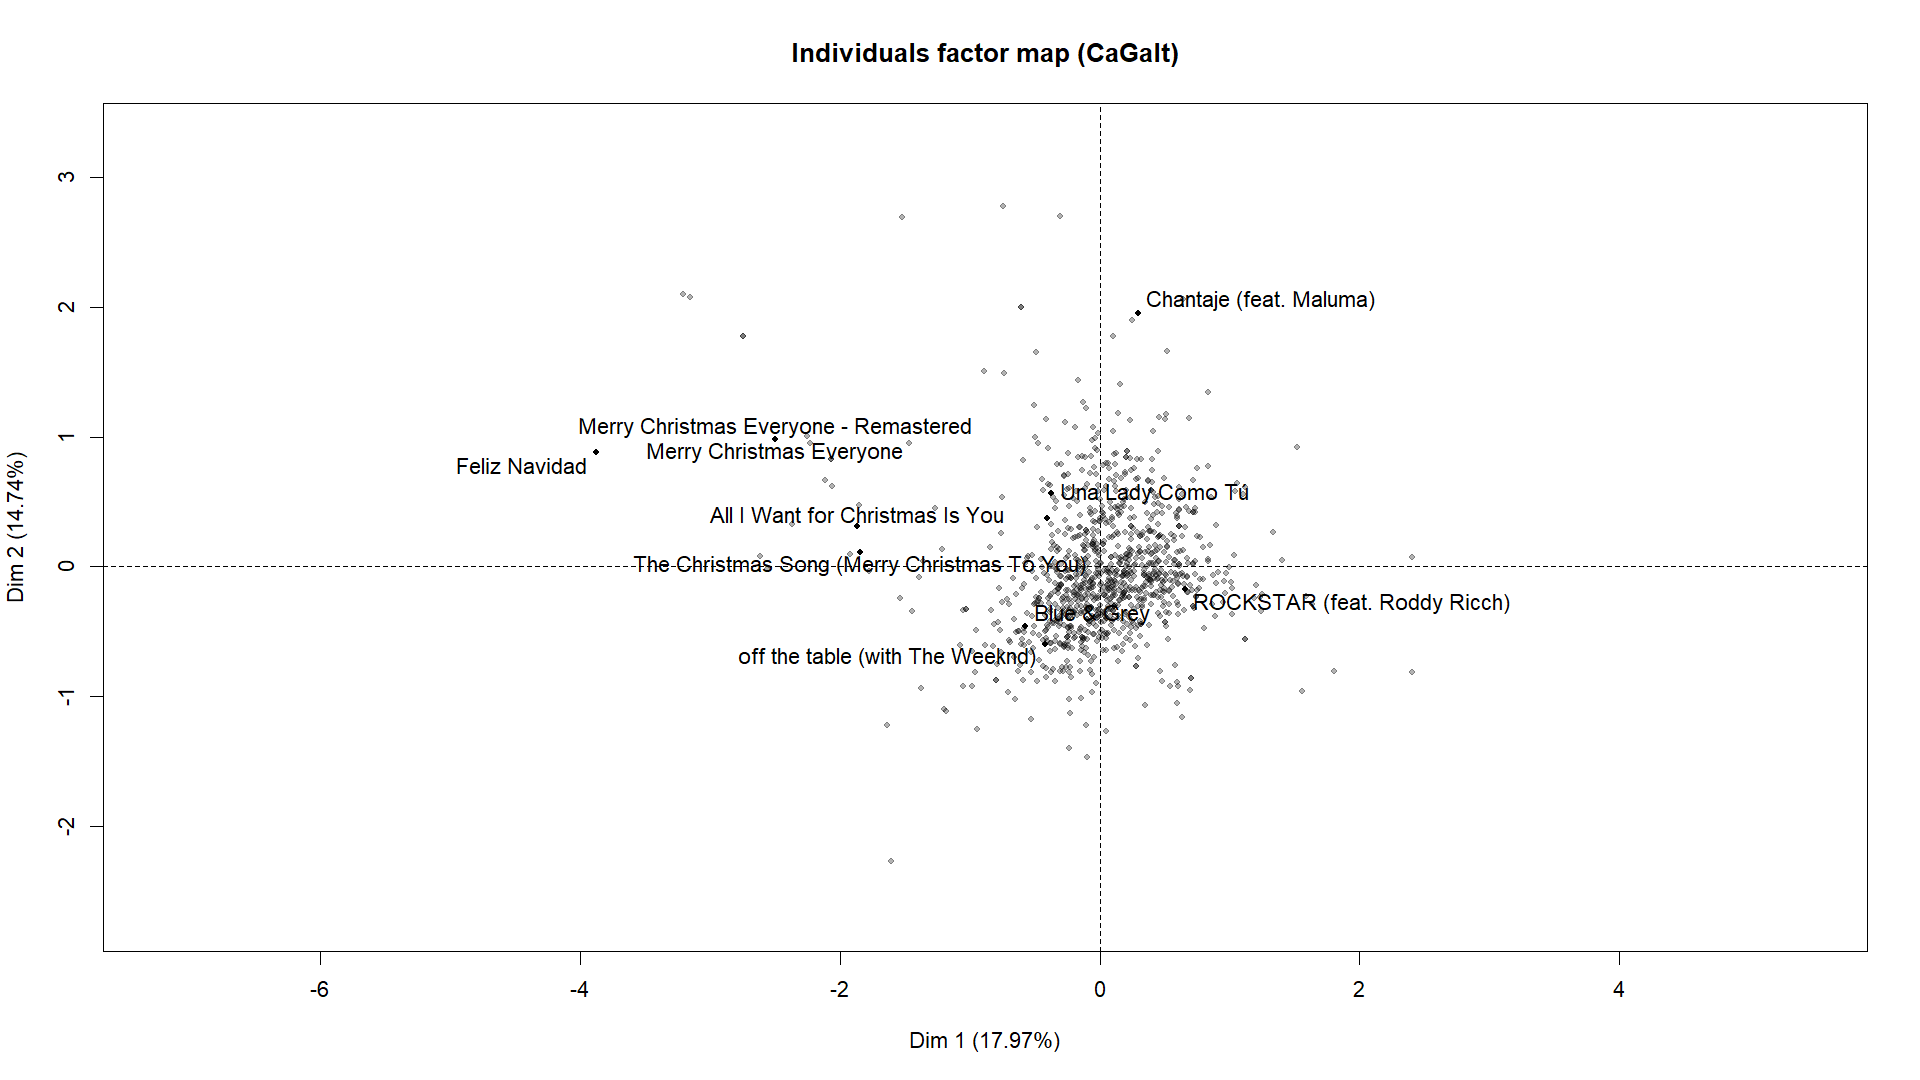
\includegraphics[width=0.7\linewidth]{Images//8_Textual//Analysis/cagalt_tracks_12.png}
    \caption{Tracks en CA-GALT amb les numèriques en les dues primeres dimensions}
    \label{fig:textual_cagaltnum_tracks12}
\end{figure}

\begin{figure}[H]
    \centering
    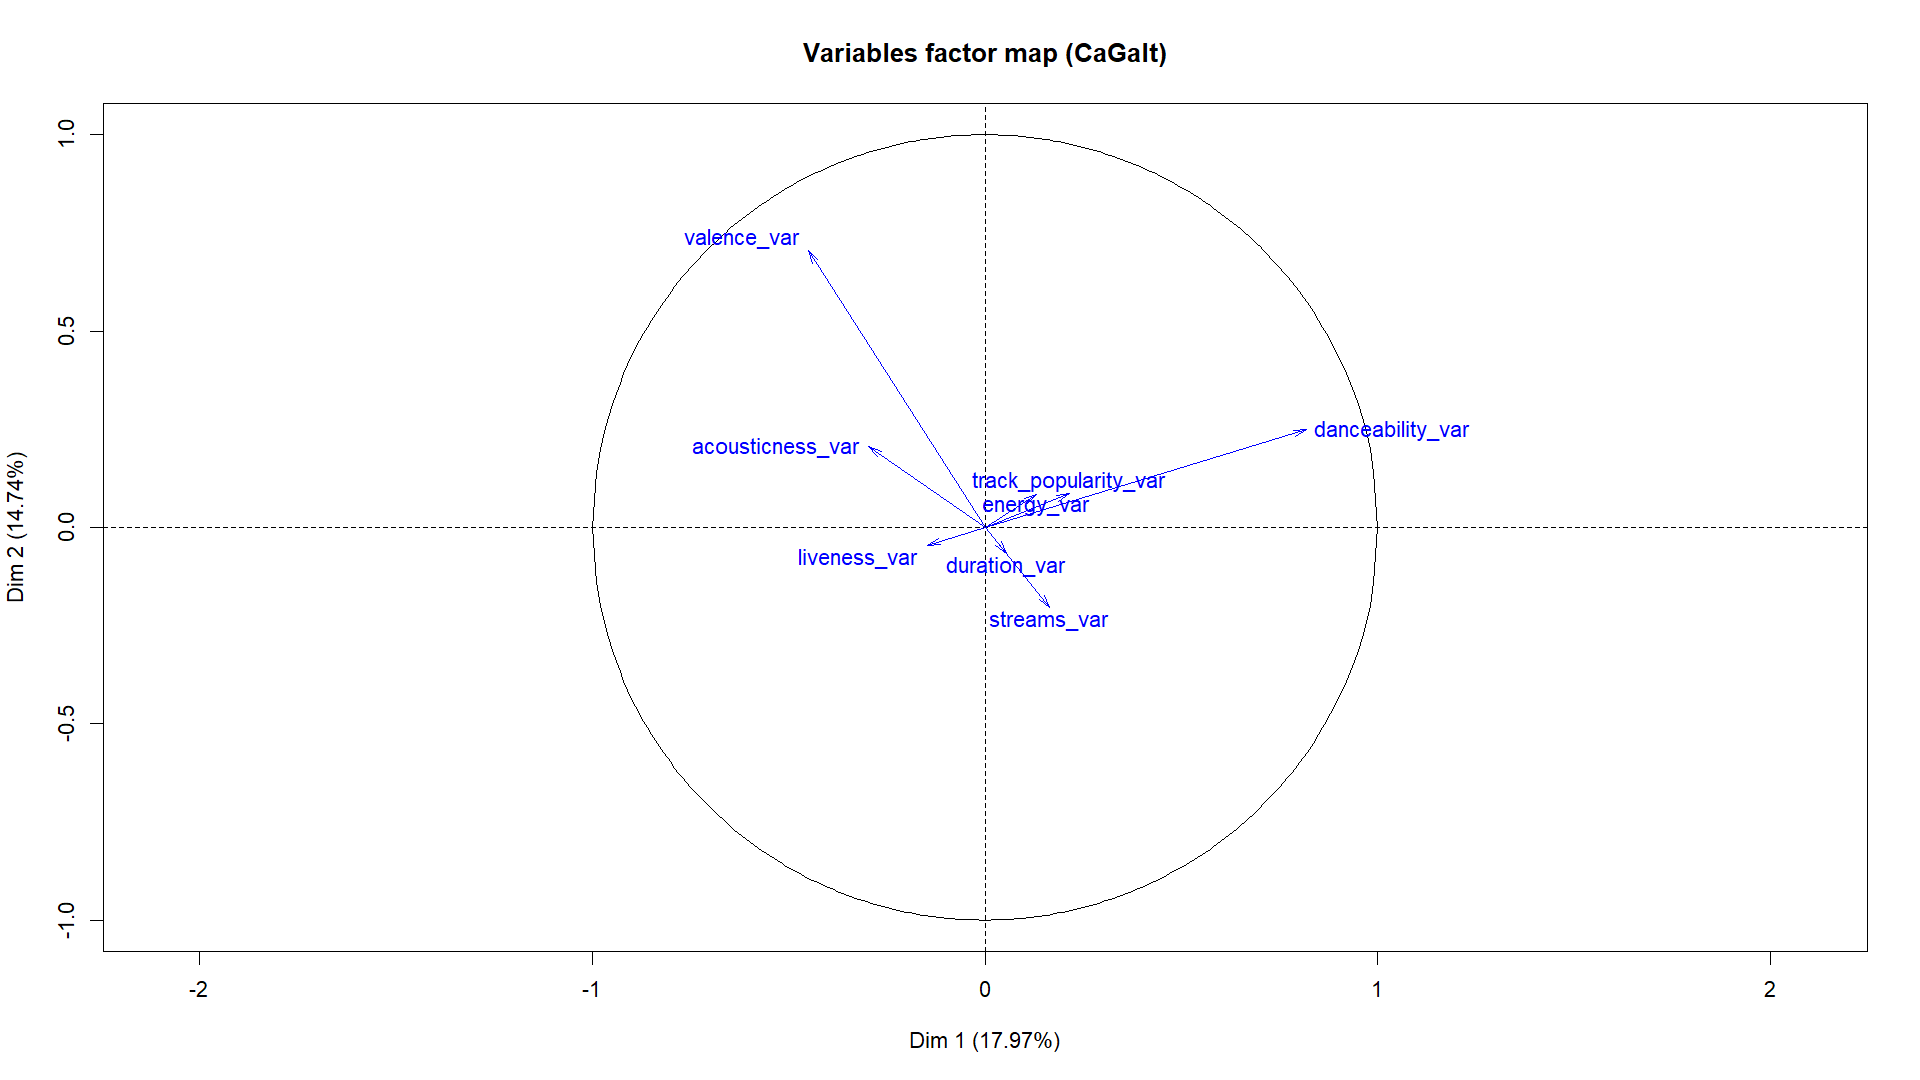
\includegraphics[width=0.7\linewidth]{Images//8_Textual//Analysis/cagalt_quanti_12.png}
    \caption{Variables en CA-GALT amb les numèriques en les dues primeres dimensions}
    \label{fig:textual_cagalnum_vars12}
\end{figure}

Observem com aquest cop, els documents estan més repartits en l'espai. La dimensió 1 (i part de la 2), en direcció negativa de la 1 i positiva de la 2, continua representant les cançons de Nadal, però en aquest cas inclou la resta (no només una) \ref{fig:textual_cagaltnum_tracks12}, \ref{fig:textual_cagaltnum_words12}. A més, veiem com la valence (positivitat) també apunta cap aquella direcció, indicant que aquest tipus de cançons (les que parlen sobre el nadal) solen ser positives també musicalment \ref{fig:textual_cagalnum_vars12}.

Valors positius de la primera dimensió també s'associen amb una dansabilitat alta, i observem com apareixen algunes cançons de reggaetón o hip hop (les que tenen nom són les tenen un cos2 més elevat). Es pot observar també la contribució de les paraules en les dimensions 1 i 2:

\begin{figure}[H]
\centering
    \begin{minipage}{.4\textwidth}
        \centering
        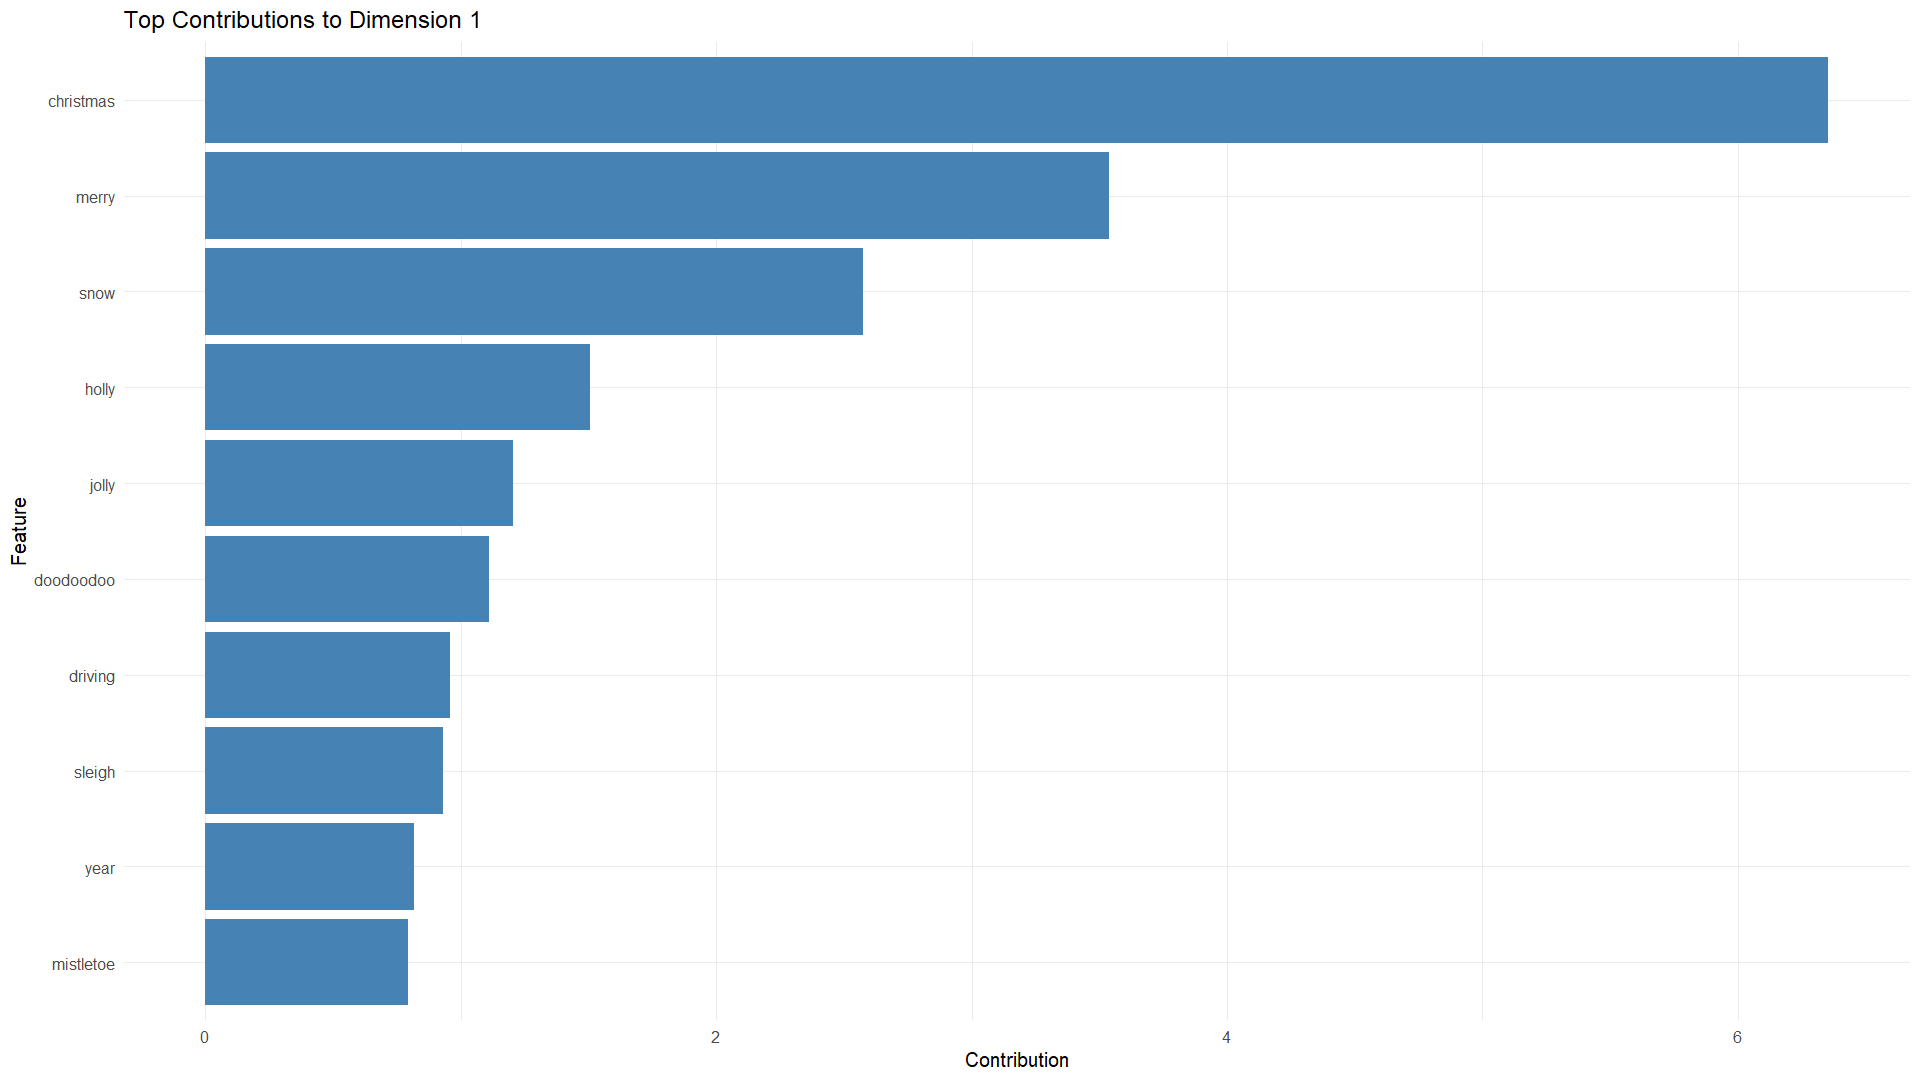
\includegraphics[width=0.95\linewidth]{Images//8_Textual//Analysis/cagalt_contrib_1.png}
        \caption{Contribució de les paraules en la primera dimensió del CA-GALT amb numèriques}
        \label{fig:textual_cagalnum_contrib1}
    \end{minipage}%
    \begin{minipage}{.4\textwidth}
        \centering
        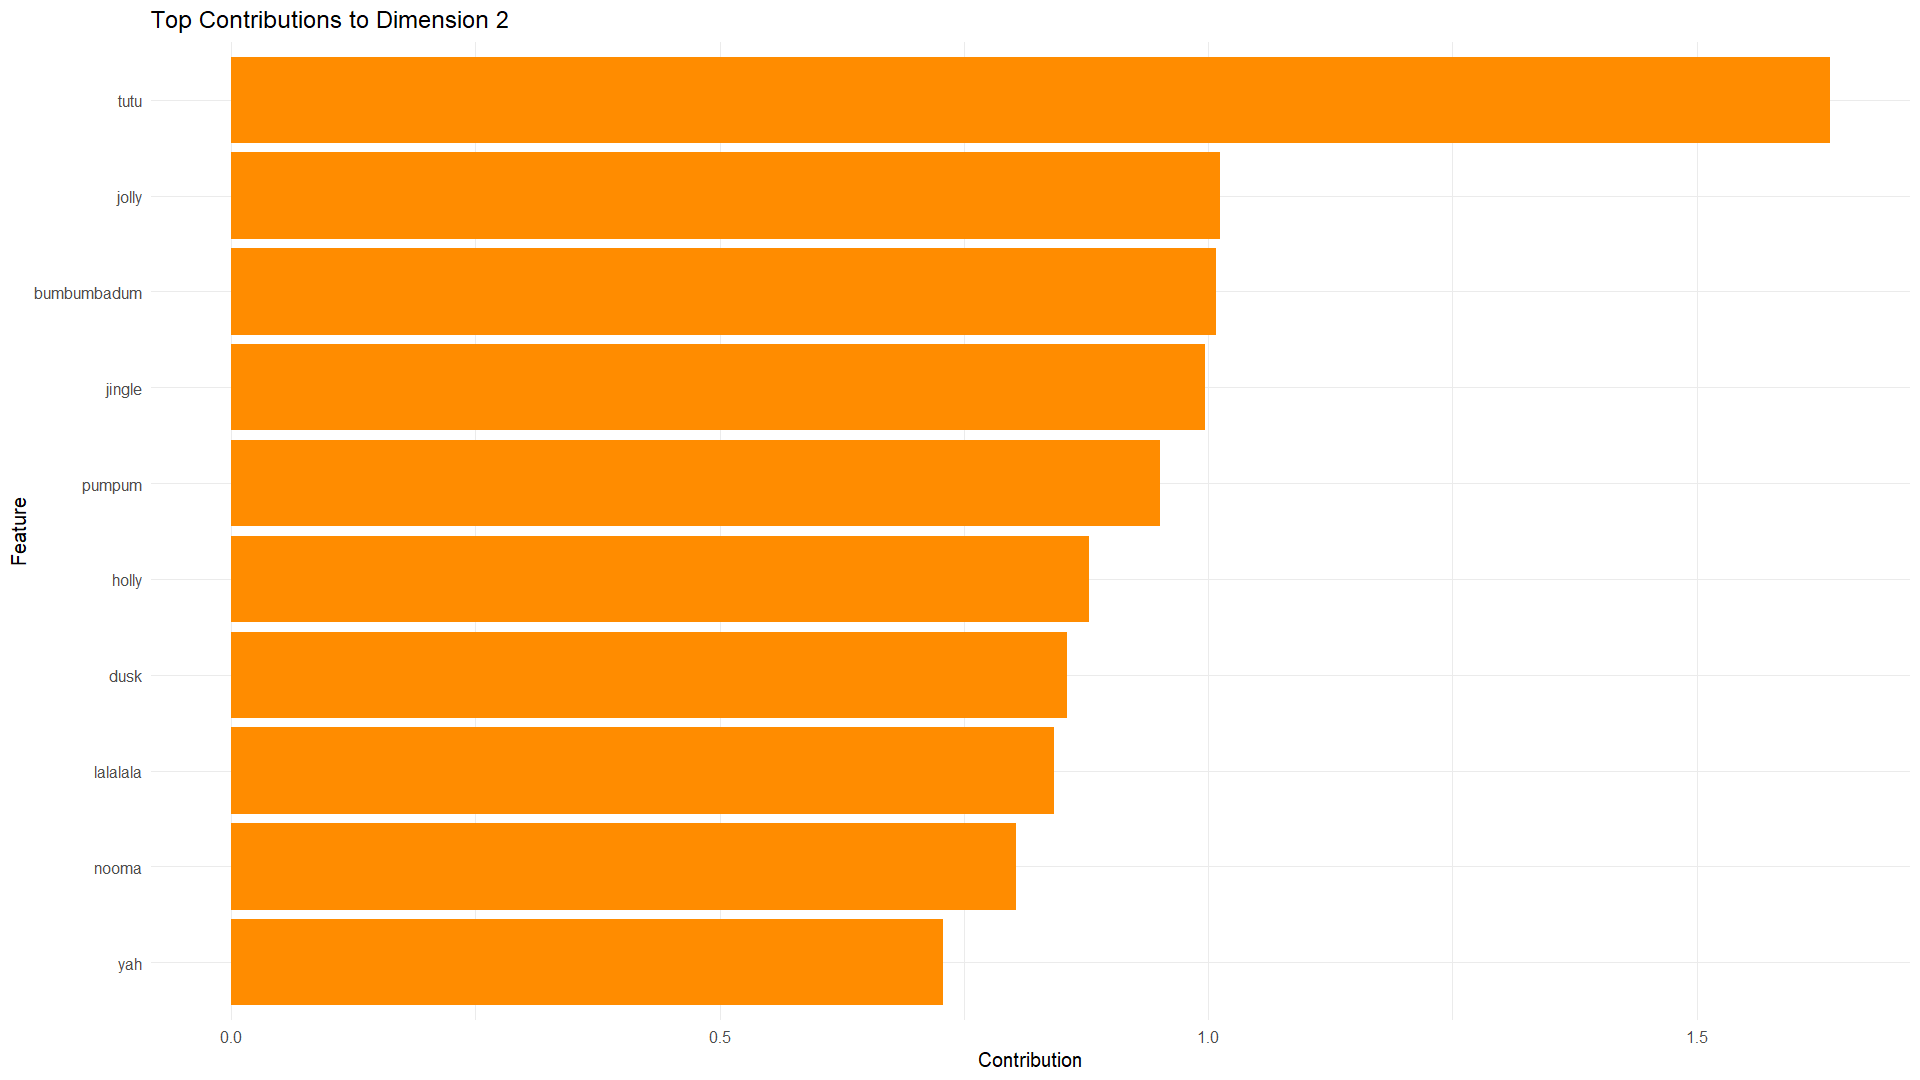
\includegraphics[width=0.95\linewidth]{Images//8_Textual//Analysis/cagalt_contrib_2.png}
        \caption{Contribució de les paraules en la primera dimensió del CA-GALT amb numèriques}
        \label{fig:textual_cagalnum_contrib2}
    \end{minipage}%
\end{figure}

La primera dimensió, com era d'esperar, ve donada per paraules relacionades amb el Nadal (\textit{christmas}, \textit{merry}, \textit{snow}...) \ref{fig:textual_cagalnum_contrib1}, mentre que en la segona apareixen més aviat recursos lírics (\textit{pumpum}, \textit{lalala}...) \ref{fig:textual_cagalnum_contrib2}.

A més de fer aquest anàlisi ajuntat les variables textuals amb les numèriques, també es pot realitzar amb les categòriques. S'han escollit les variables corresponents als gèneres musicals, així com explicit i el gènere dels artistes per aquest. La primera dimensió, en aquest nou CA-GALT, explica un 19.77\%, tot i que la segona cau ràpidament a un 12.34\%.

\begin{figure}[H]
    \centering
    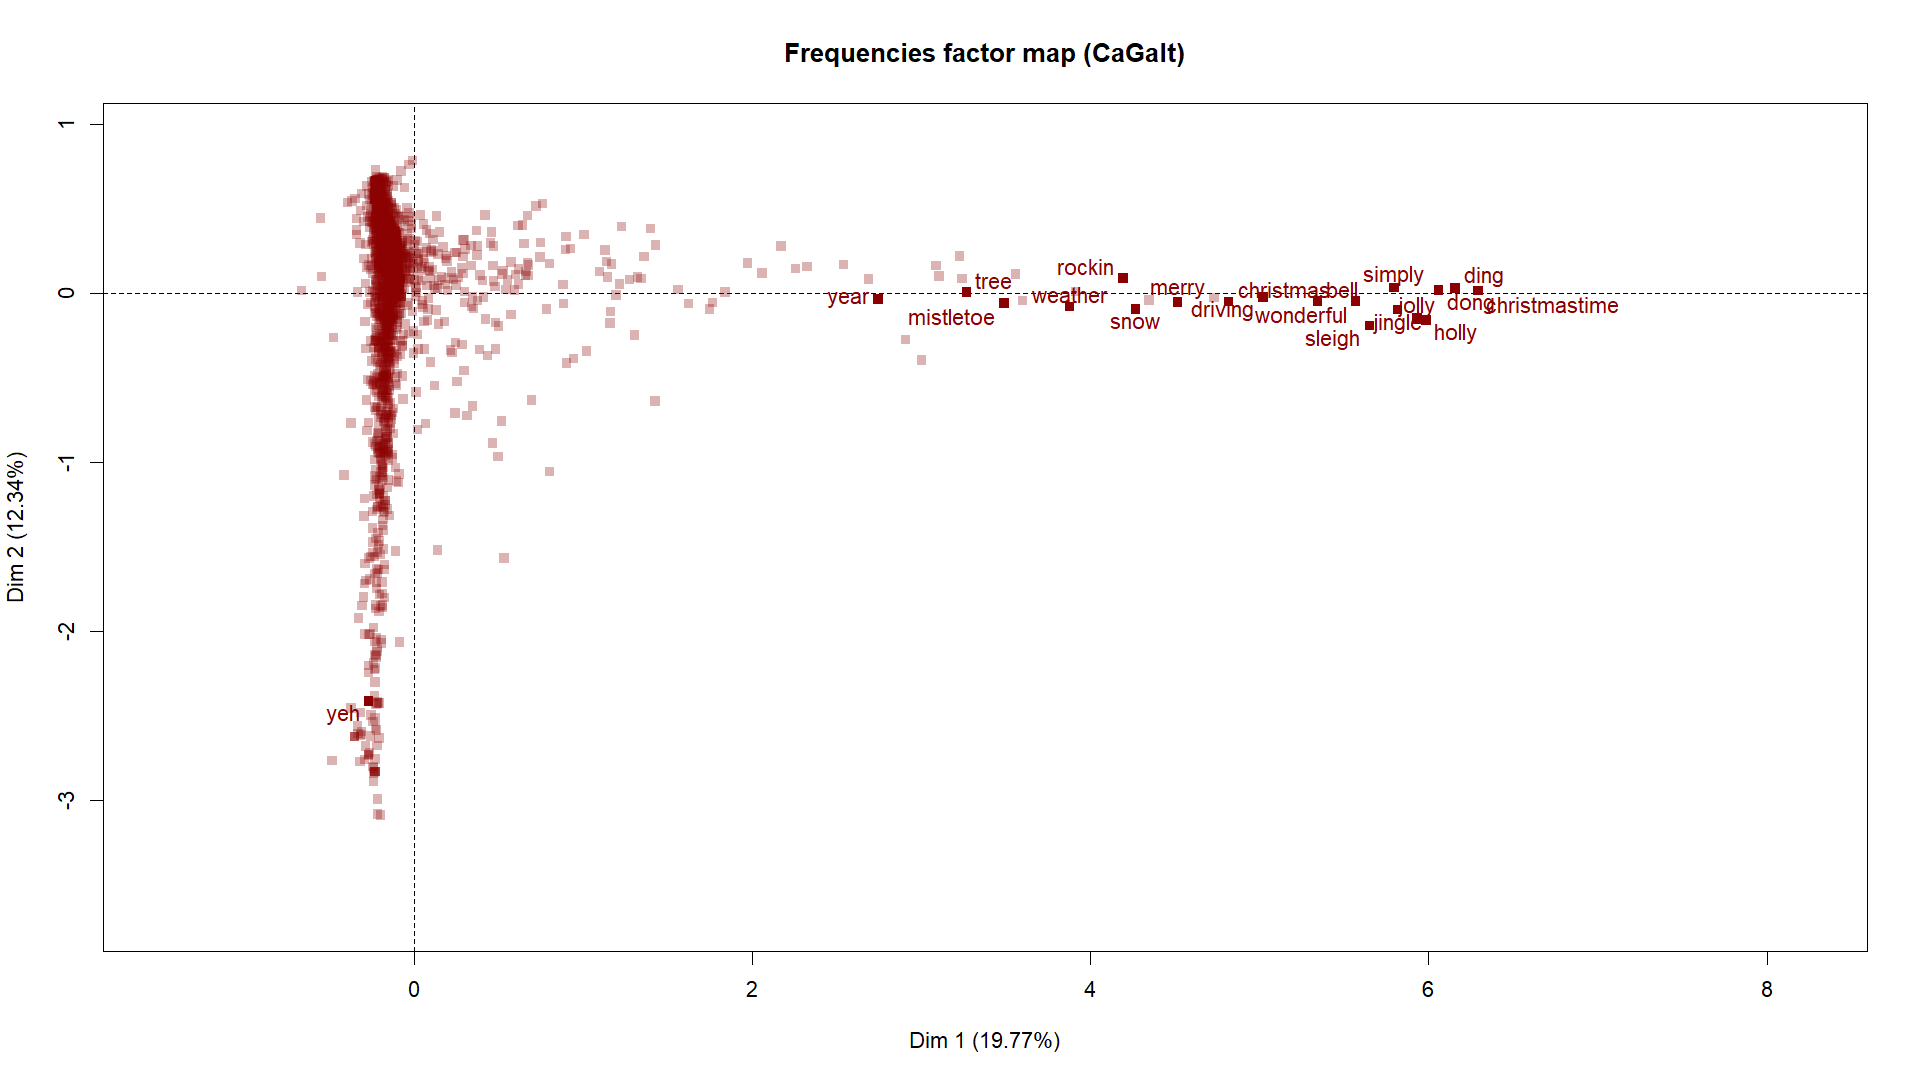
\includegraphics[width=0.7\linewidth]{Images//8_Textual//Analysis/cagalt2_words_12.png}
    \caption{Paraules en CA-GALT amb categòriques en les dues primeres dimensions}
    \label{fig:textual_cagaltcat_words12}
\end{figure}

\begin{figure}[H]
    \centering
    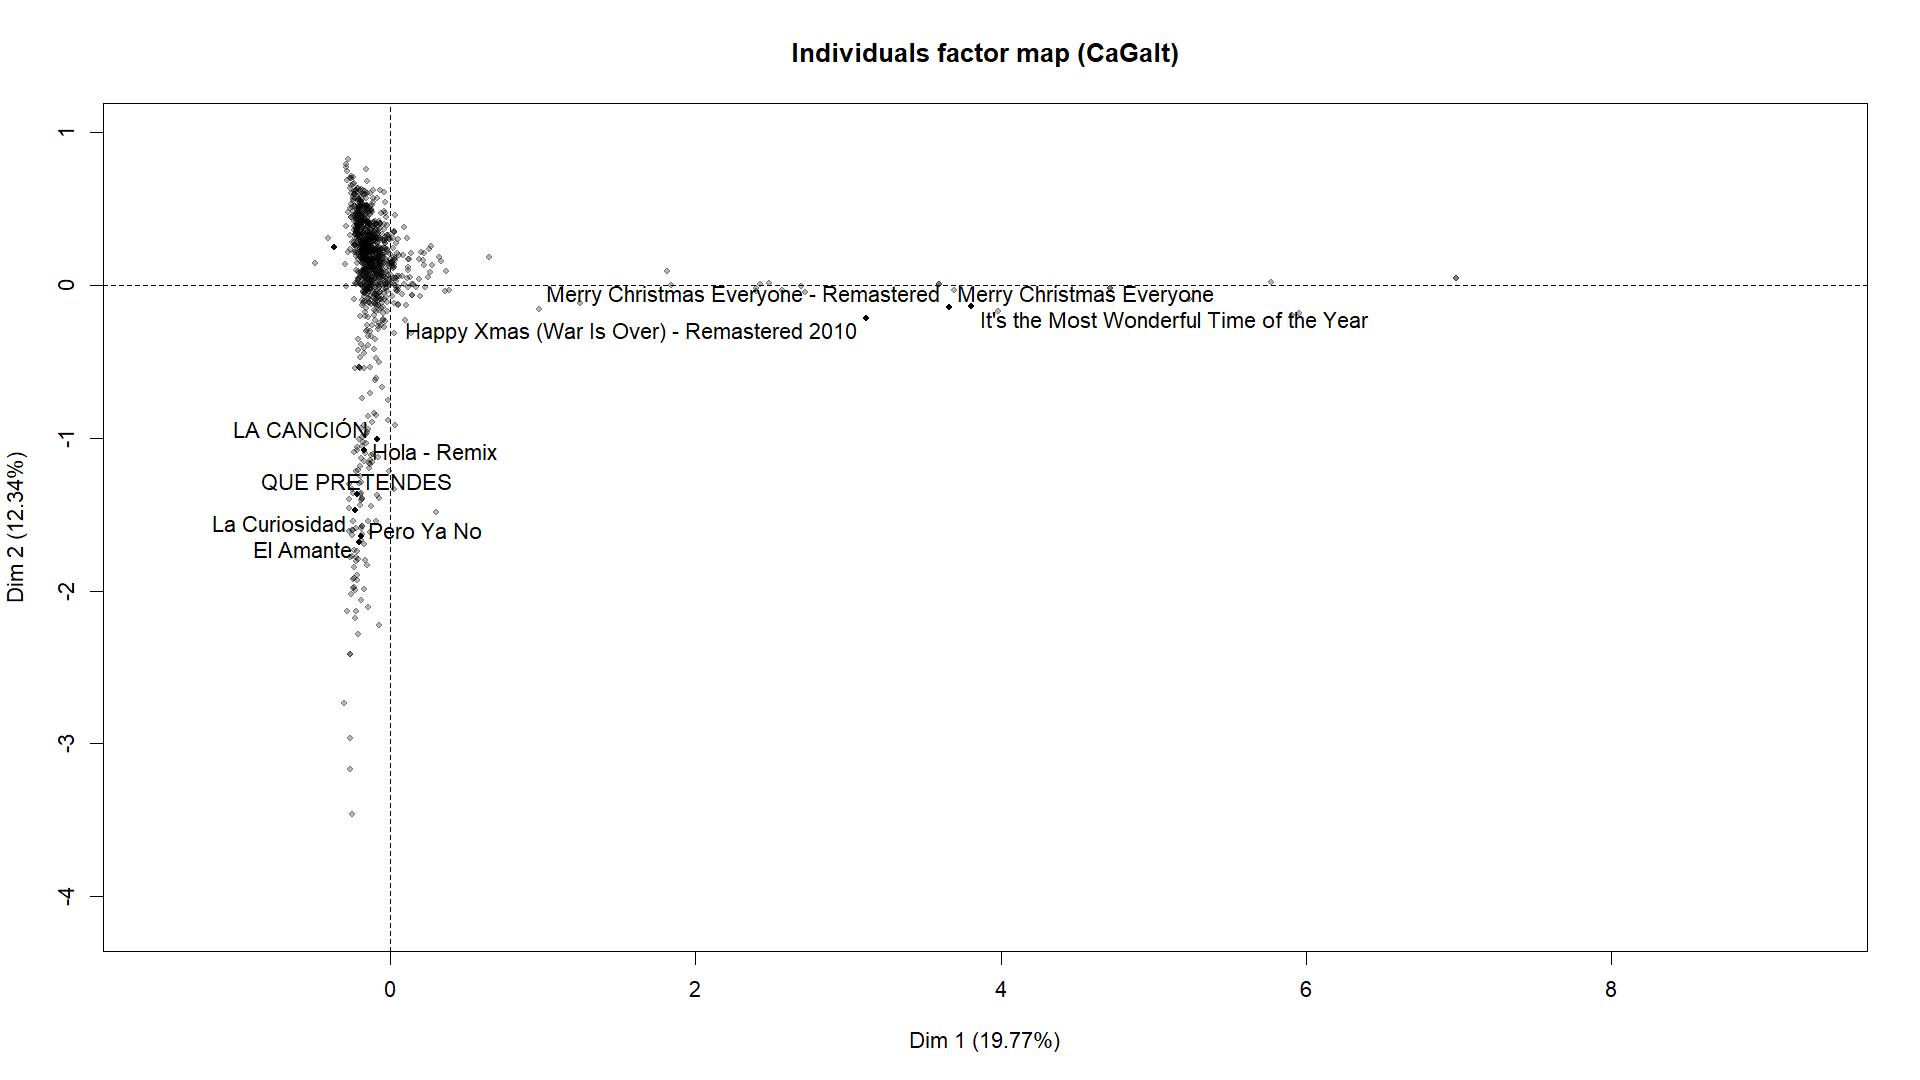
\includegraphics[width=0.7\linewidth]{Images//8_Textual//Analysis/cagalt2_tracks_12.png}
    \caption{Tracks en CA-GALT amb categòriques en les dues primeres dimensions}
    \label{fig:textual_cagaltcat_tracks12}
\end{figure}

\begin{figure}[H]
    \centering
    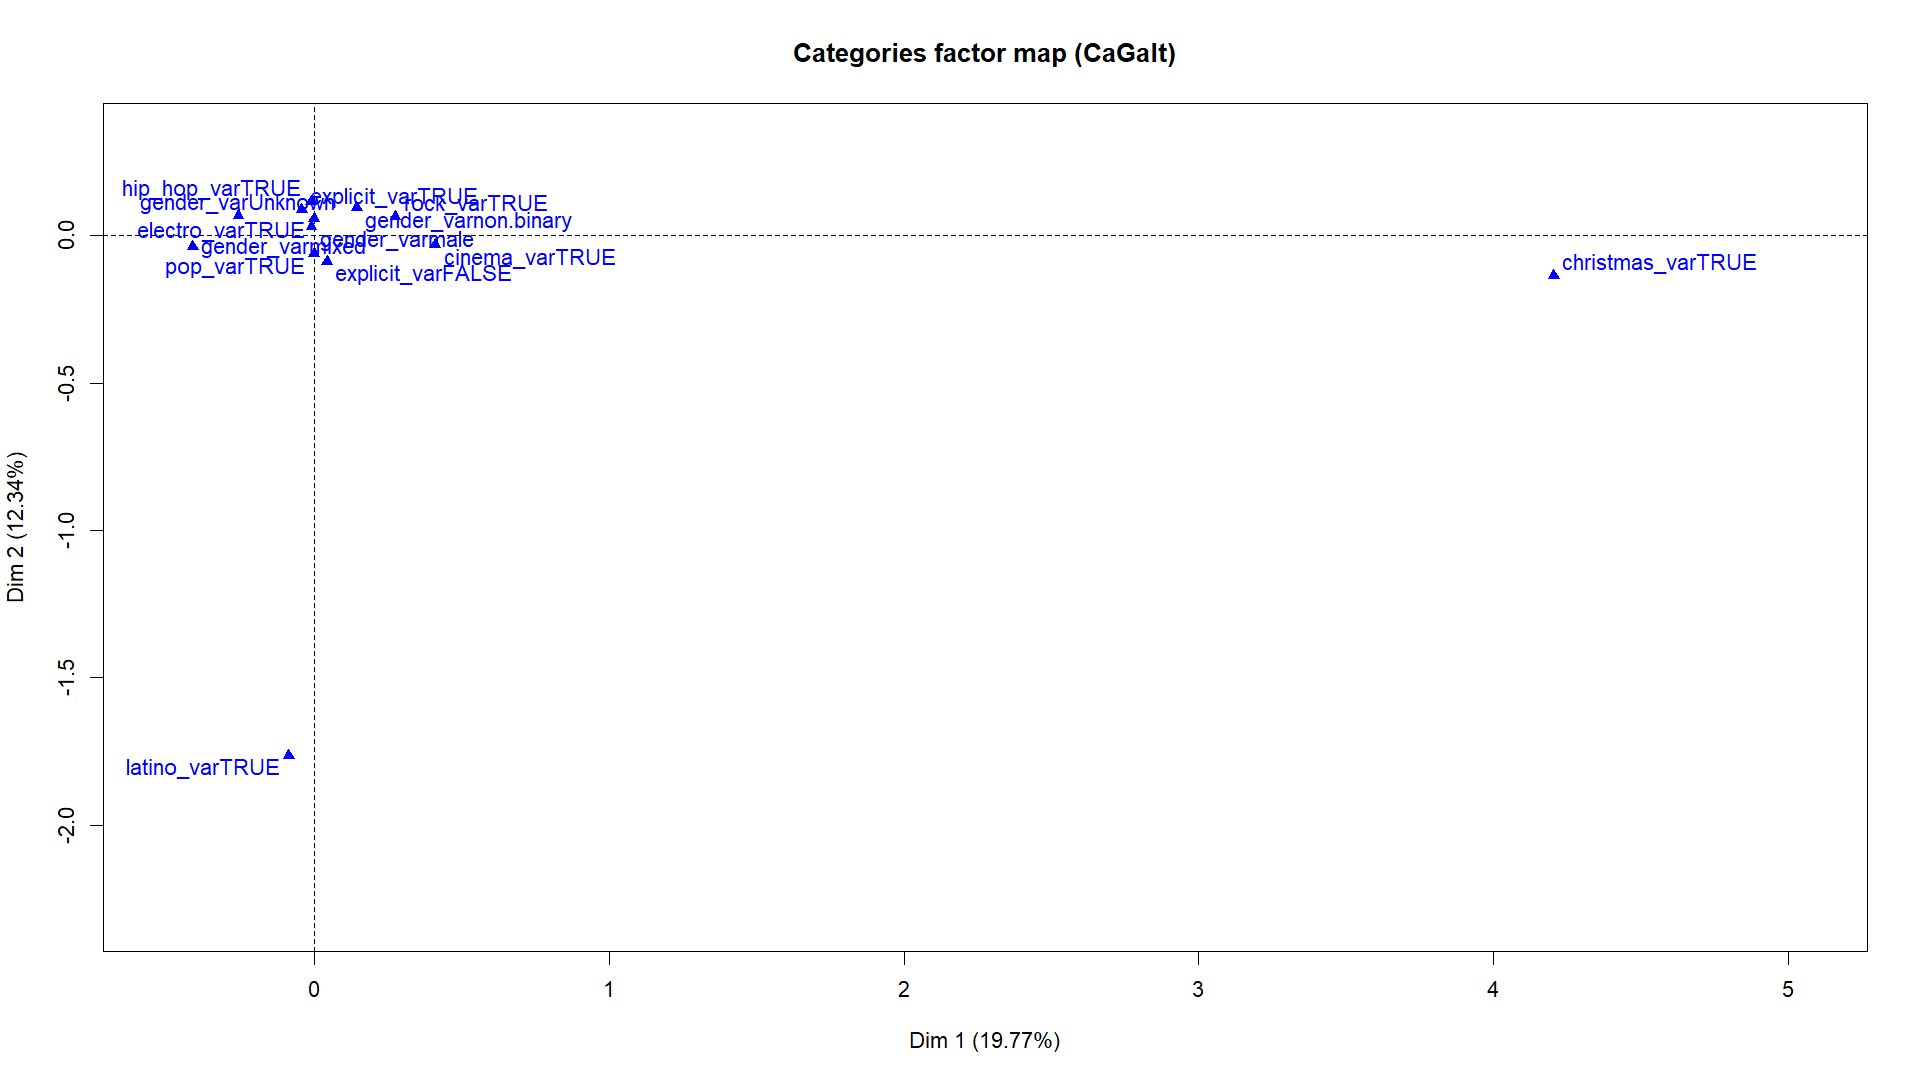
\includegraphics[width=0.7\linewidth]{Images//8_Textual//Analysis/cagalt2_quali_12.png}
    \caption{Variables en CA-GALT amb categòriques en les dues primeres dimensions}
    \label{fig:textual_cagaltcat_vars12}
\end{figure}

En aquest cas, tornem a trobar els tracks ajuntats en els eixos, però millor que en el CA original. Observem com clarament la dimensió 1 ve altre cop determinada per les cançons de Nadal, i en aquest cas la 2 per les de reggaetó (\ref{fig:textual_cagaltcat_words12}, \ref{fig:textual_cagaltcat_tracks12} i \ref{fig:textual_cagaltcat_vars12}). De fet, en les paraules que contribueixen apareixen algunes com \textit{perreate}, \textit{criminal}, \textit{tutu}, \textit{yeh}... (algunes en castellà, però escrites malament i que per tant no s'han traduït).

\begin{figure}[H]
\centering
    \begin{minipage}{.4\textwidth}
        \centering
        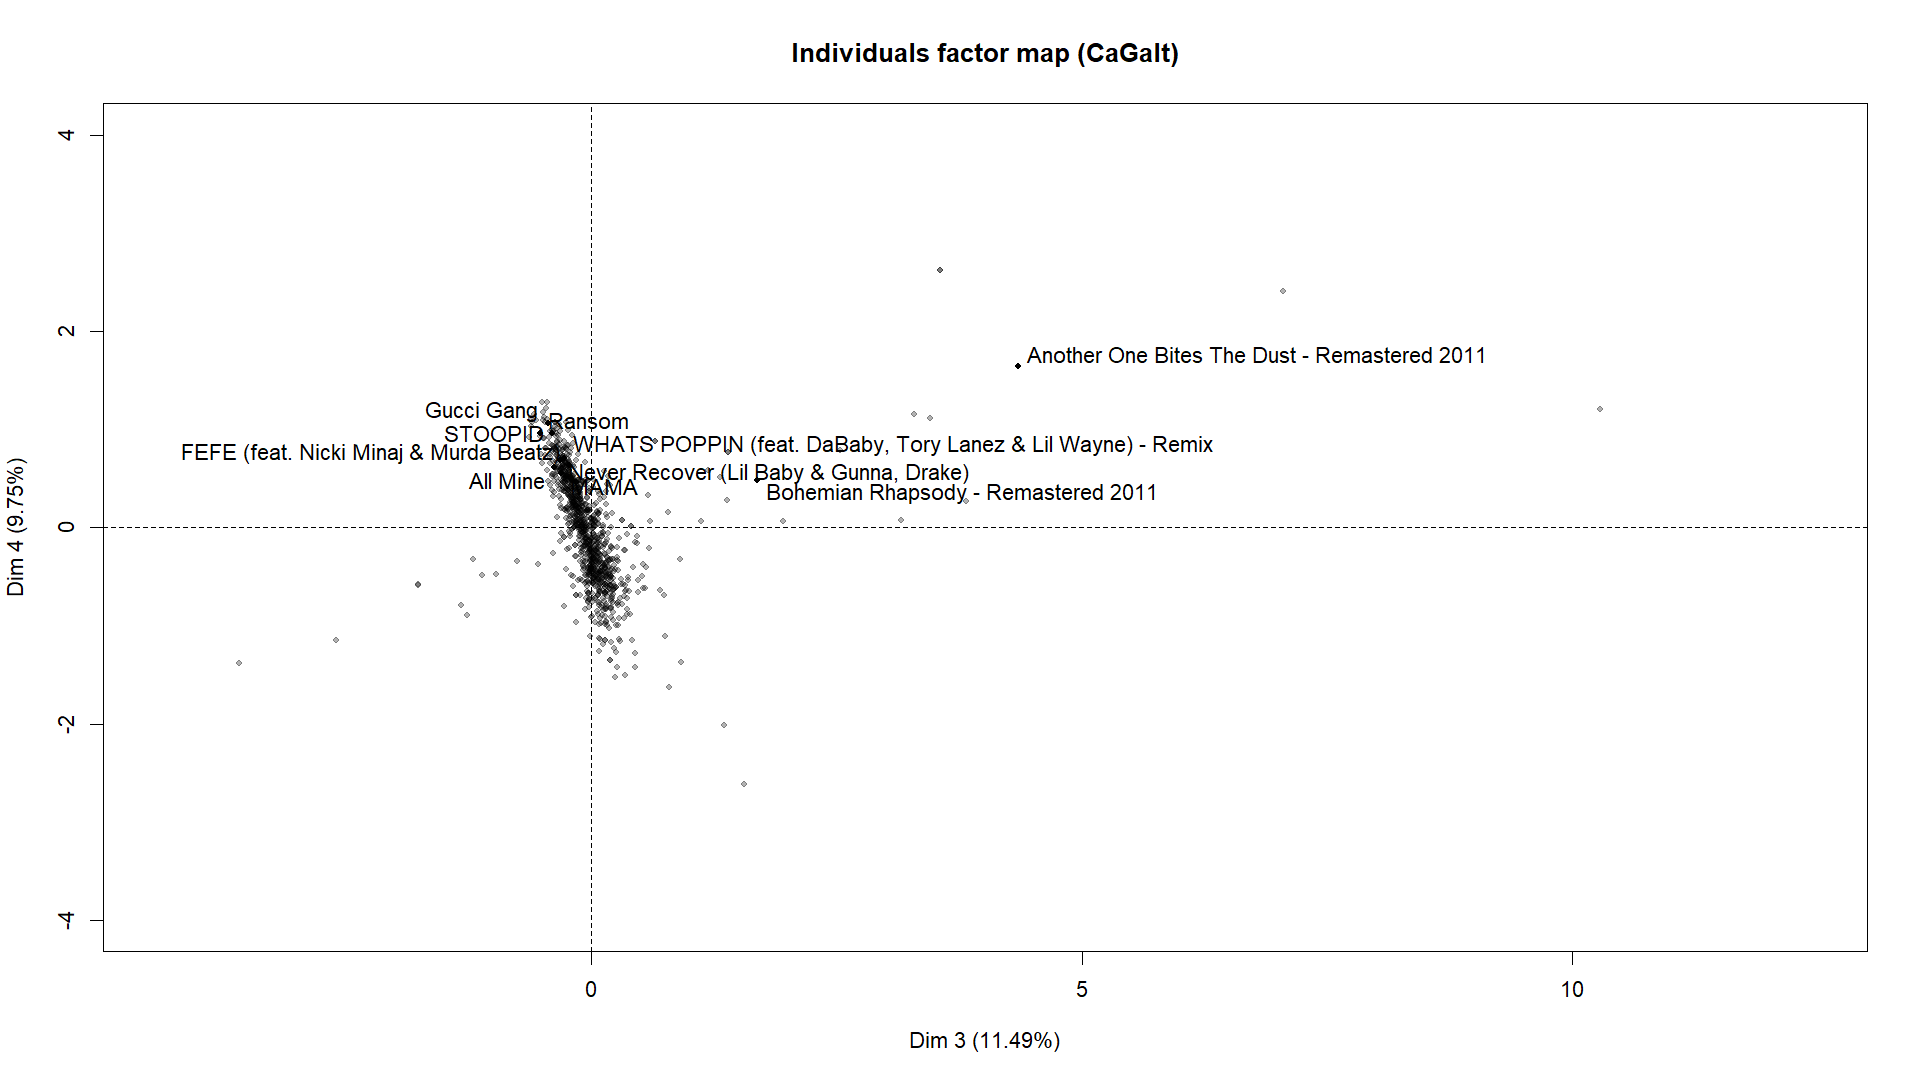
\includegraphics[width=0.95\linewidth]{Images//8_Textual//Analysis/cagalt2_tracks_34.png}
        \caption{Tracks en CA-GALT amb categòriques en les dimensions 3 i 4}
        \label{fig:textual_cagaltcat_tracks34}
    \end{minipage}%
    \begin{minipage}{.4\textwidth}
        \centering
        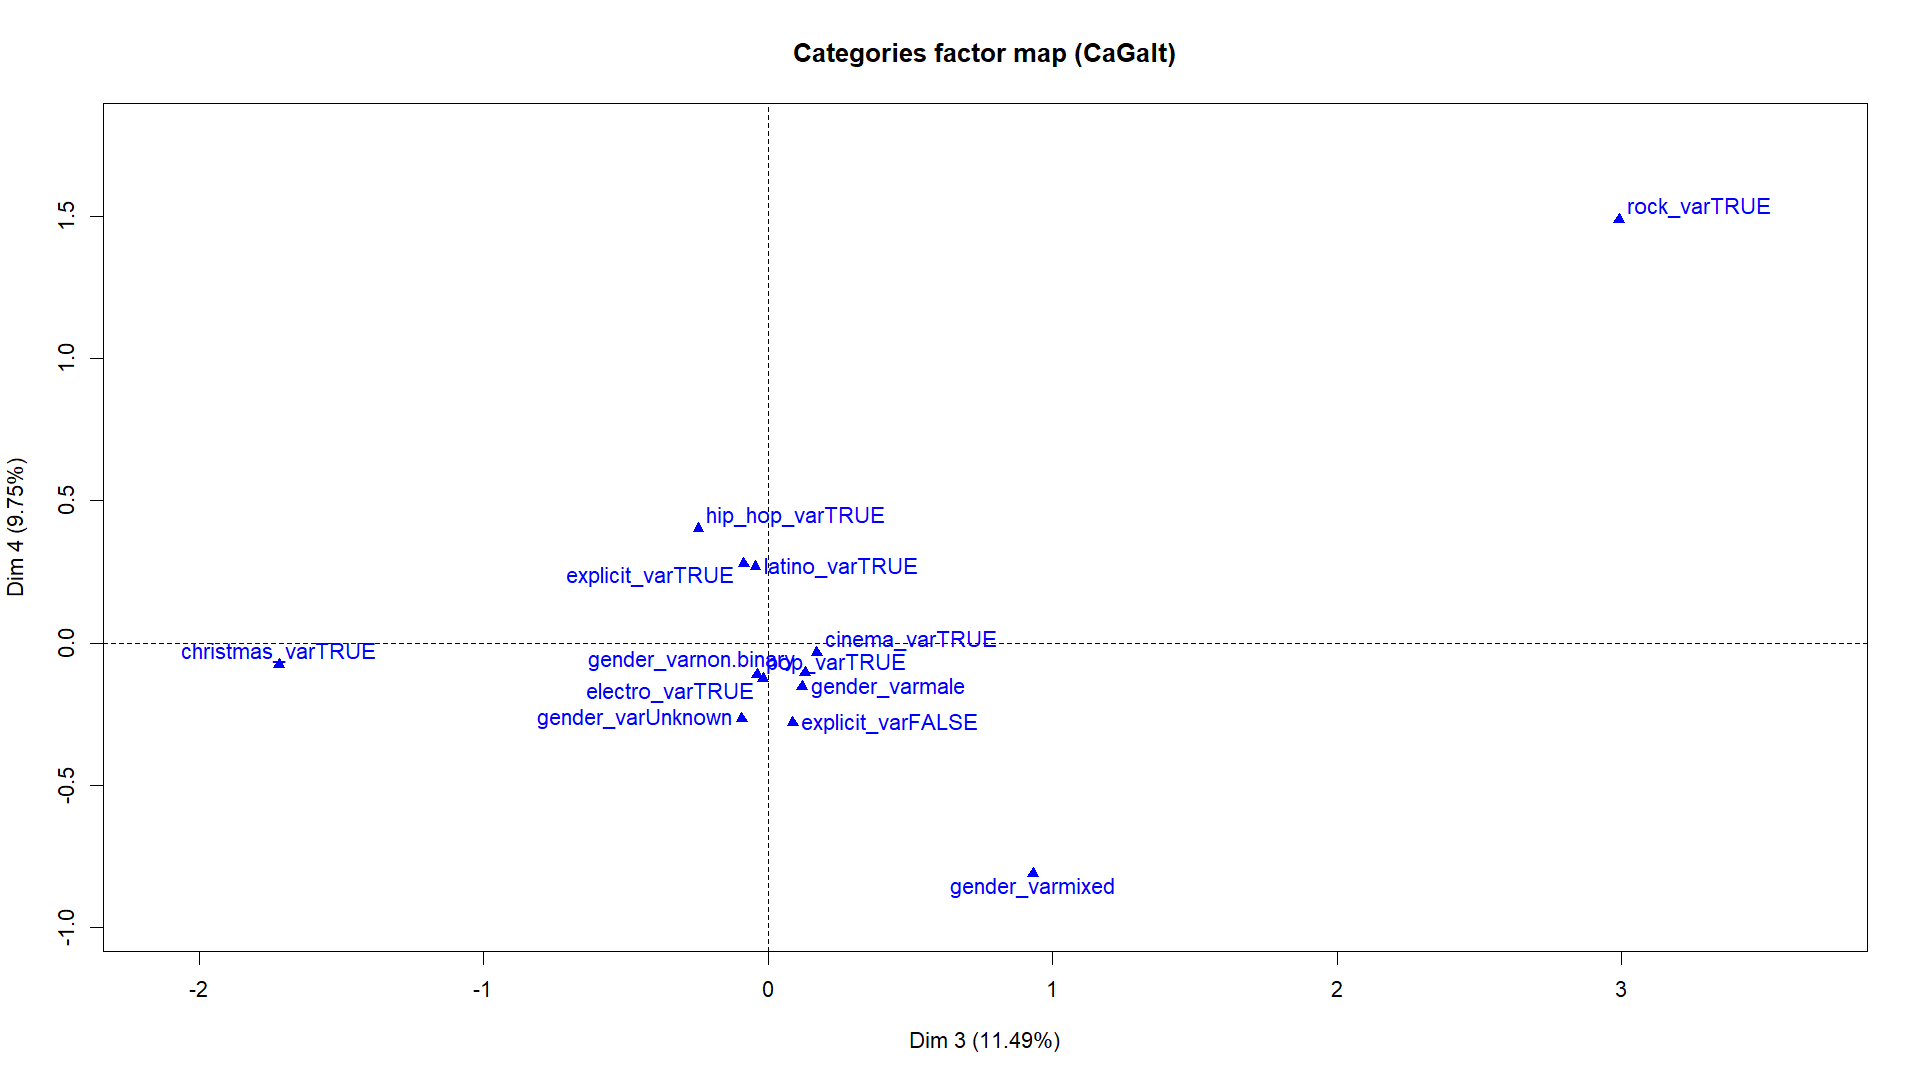
\includegraphics[width=0.95\linewidth]{Images//8_Textual//Analysis/cagalt2_quali_34.png}
        \caption{Variables en CA-GALT amb categòriques en les dimensions 3 i 4}
        \label{fig:textual_cagaltcat_vars34}
    \end{minipage}%
\end{figure}

En les següents dimensions (\ref{fig:textual_cagaltcat_tracks34} i \ref{fig:textual_cagaltcat_vars34}), s'intueix en certa manera com les cançons de hip hop se situen en valors negatius de la dimensió 3 i positius de la 4, relacionant-se amb la variable hip\_hop true.


En conclusió, gràcies a aquest anàlisi de correspondències, i especialment al fet d'afegir més variables, hem pogut observar com sembla ser que la lletra de la cançó està relacionada en certa manera amb com de ballable és una cançó, com de positiva, o bé de quin gènere musical seria. 

\subsection{Anàlisi Semàntic Latent}\label{LSA}

L'anàlisi semantic latent, o LSA, permet aprofundir més en les relacions textuals entre els documents i les paraules, i obtenir un espai on poder comparar similituds de forma més senzilla en una respresentació vectorial d'aquests.

Aquesta anàlisi s'ha realitzat dos cops: amb les dades sense traduïr i amb les traduïdes.

\subsubsection{Preprocessament dels textos}
El primer pas per poder dur a terme aquesta anàlisi ha sigut realitzar un preprocessament del text. Aquest ha consistit bàsicament en l'eliminació de stopwords, nombres, espais, puntuació... (en definitiva, paraules que no aportaven informació rellevant). A més, també s'han escollit només les paraules que apareixien mínim en un 10\% dels documents, per tal d'evitar una dimensionalitat massa alta i obtenir només les paraules significants

Un cop realitzat aquest preprocessament al corpus, es crea una TermDocumentMatrix, que permet relacionar les paraules amb els documents, i "pesen" utilitzant TF-IDF per tal de donar més importància a aquelles paraules freqüents en el text però infreqüents en el corpus.

\subsubsection{Espai vectorial}

El següent ha sigut, partint d'aquesta matriu, utilitzar la funció lsa per tal d'obtenir l'espai vectorial de l'LSA.

En aquest, s'ha optat per no definir una k d'entrada, que simplement selecciona el nombre de topics que ens interessen. Més endavant, provarem amb un nombre de topics més reduït, però d'entrada ens quedarem amb tots.

En aquest espai vectorial (traduït), podem per exemple comparar paraules utilitzant la similitud de cosinus: \textit{love} té un 0.617 de similitud amb \textit{baby}, mentre que tan sols 0.166 amb \textit{star} (no tenen res a veure).

També podem comparar documents (cançons) utilitzant la similitud de pearson. Per exemple, la cançó \textit{Better now} de Post Malone té 0.2287 de correlació amb \textit{Lucid Dreams} de Travis Scott, ja que les dues són cançons amb temes similars: parlen de relacions passades, amb cert sentiment de lamentació i de desamor. En canvi, la mateixa cançó tan sols té -0.0458 amb \textit{Safaera}, una cançó de Bad Bunny que tracta sobre la festa, desitjos sexuals i en general és més positiva.

Com es pot apreciar, aquest espai ens permet relacionar bastant bé aquestes cançons i paraules entre si. 

\subsubsection{Visualització en l'espai}
Utilitzant MDS (multi dimensional scaling), podem visualitzar les paraules (\ref{fig:textual_lsa_original_50w}, \ref{fig:textual_lsa_trans_50w}) i els documents (plot\_wordlist i plot\_doclist), tant del corpus traduït com de l'original (\ref{fig:textual_lsa_original_allsongsMDS}, \ref{fig:textual_lsa_trans_allsongsMDS}).

\begin{figure}[H]
    \centering
    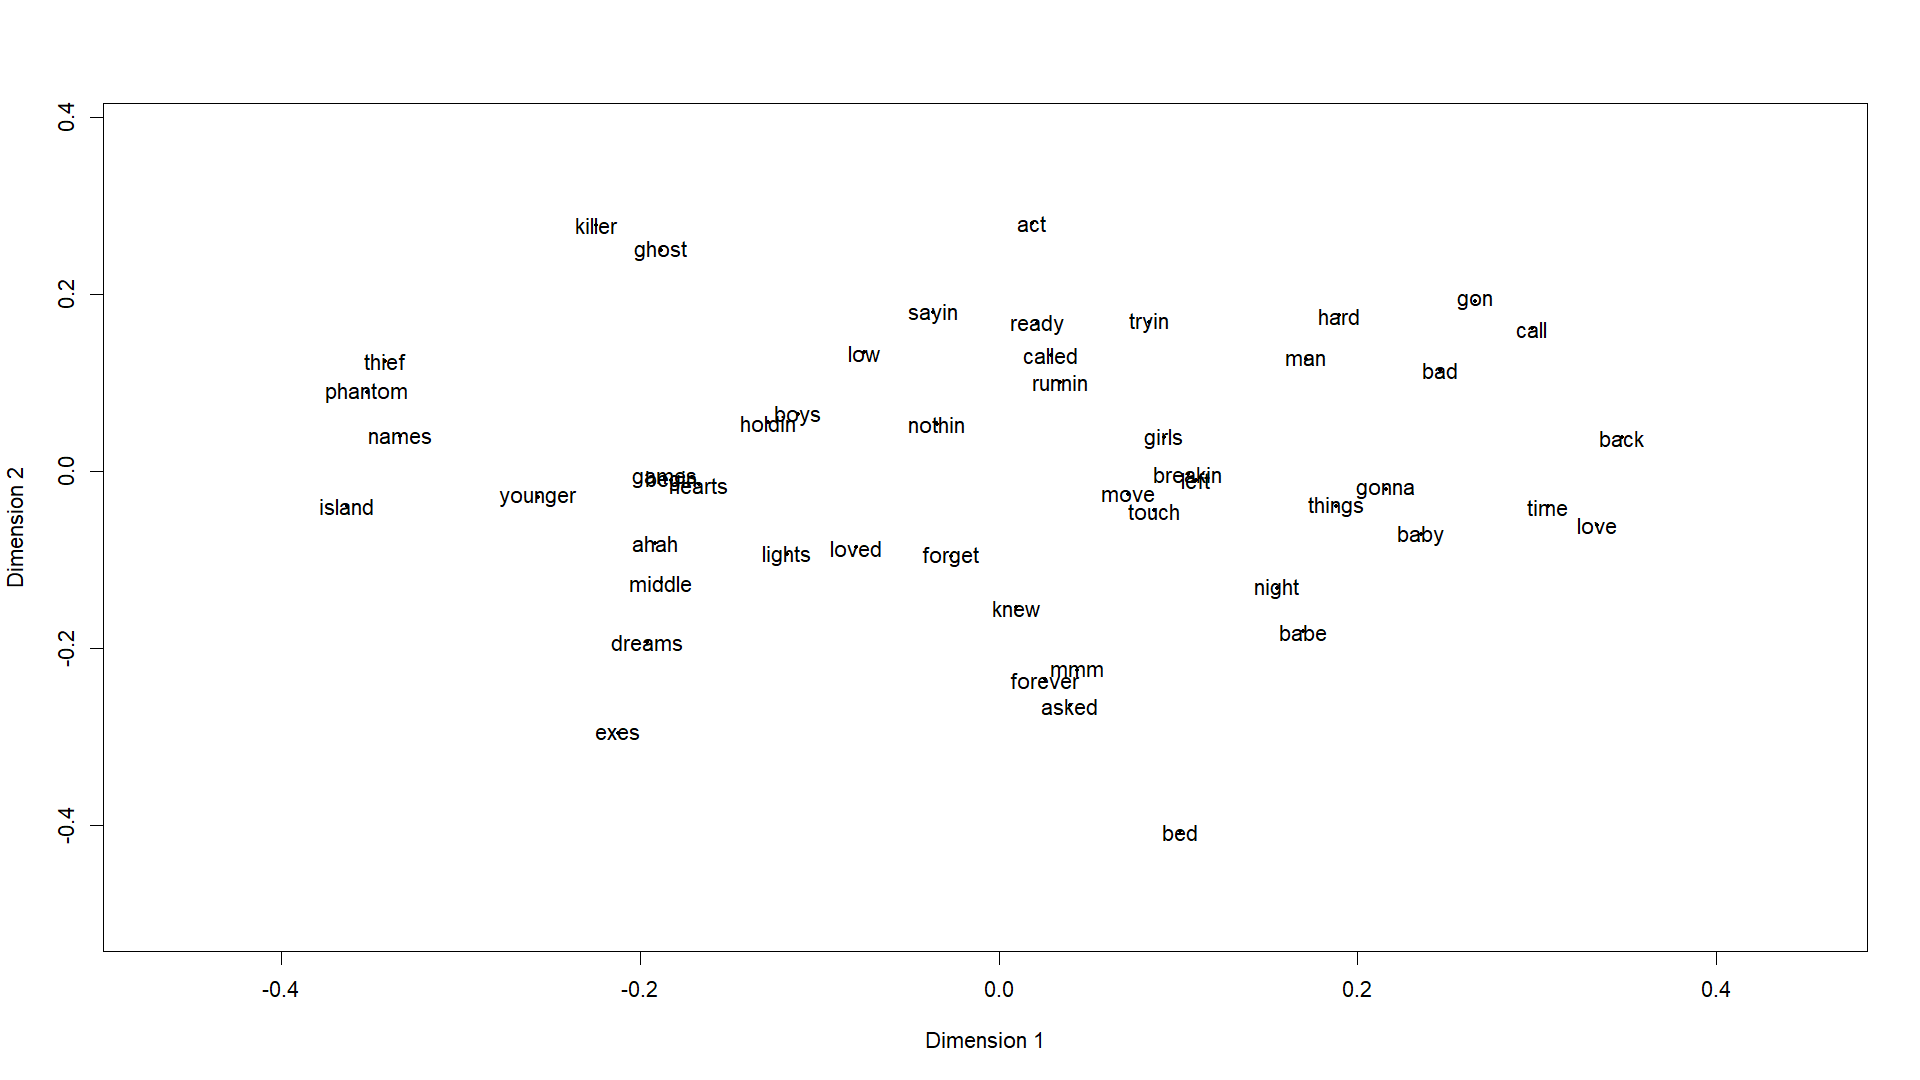
\includegraphics[width=0.8\linewidth]{Images//8_Textual//LSA/orignal_first_50_words.png}
    \caption{Primeres 50 paraules en l'MDS de l'LSA original}
    \label{fig:textual_lsa_original_50w}
\end{figure}


\begin{figure}[H]
\centering
    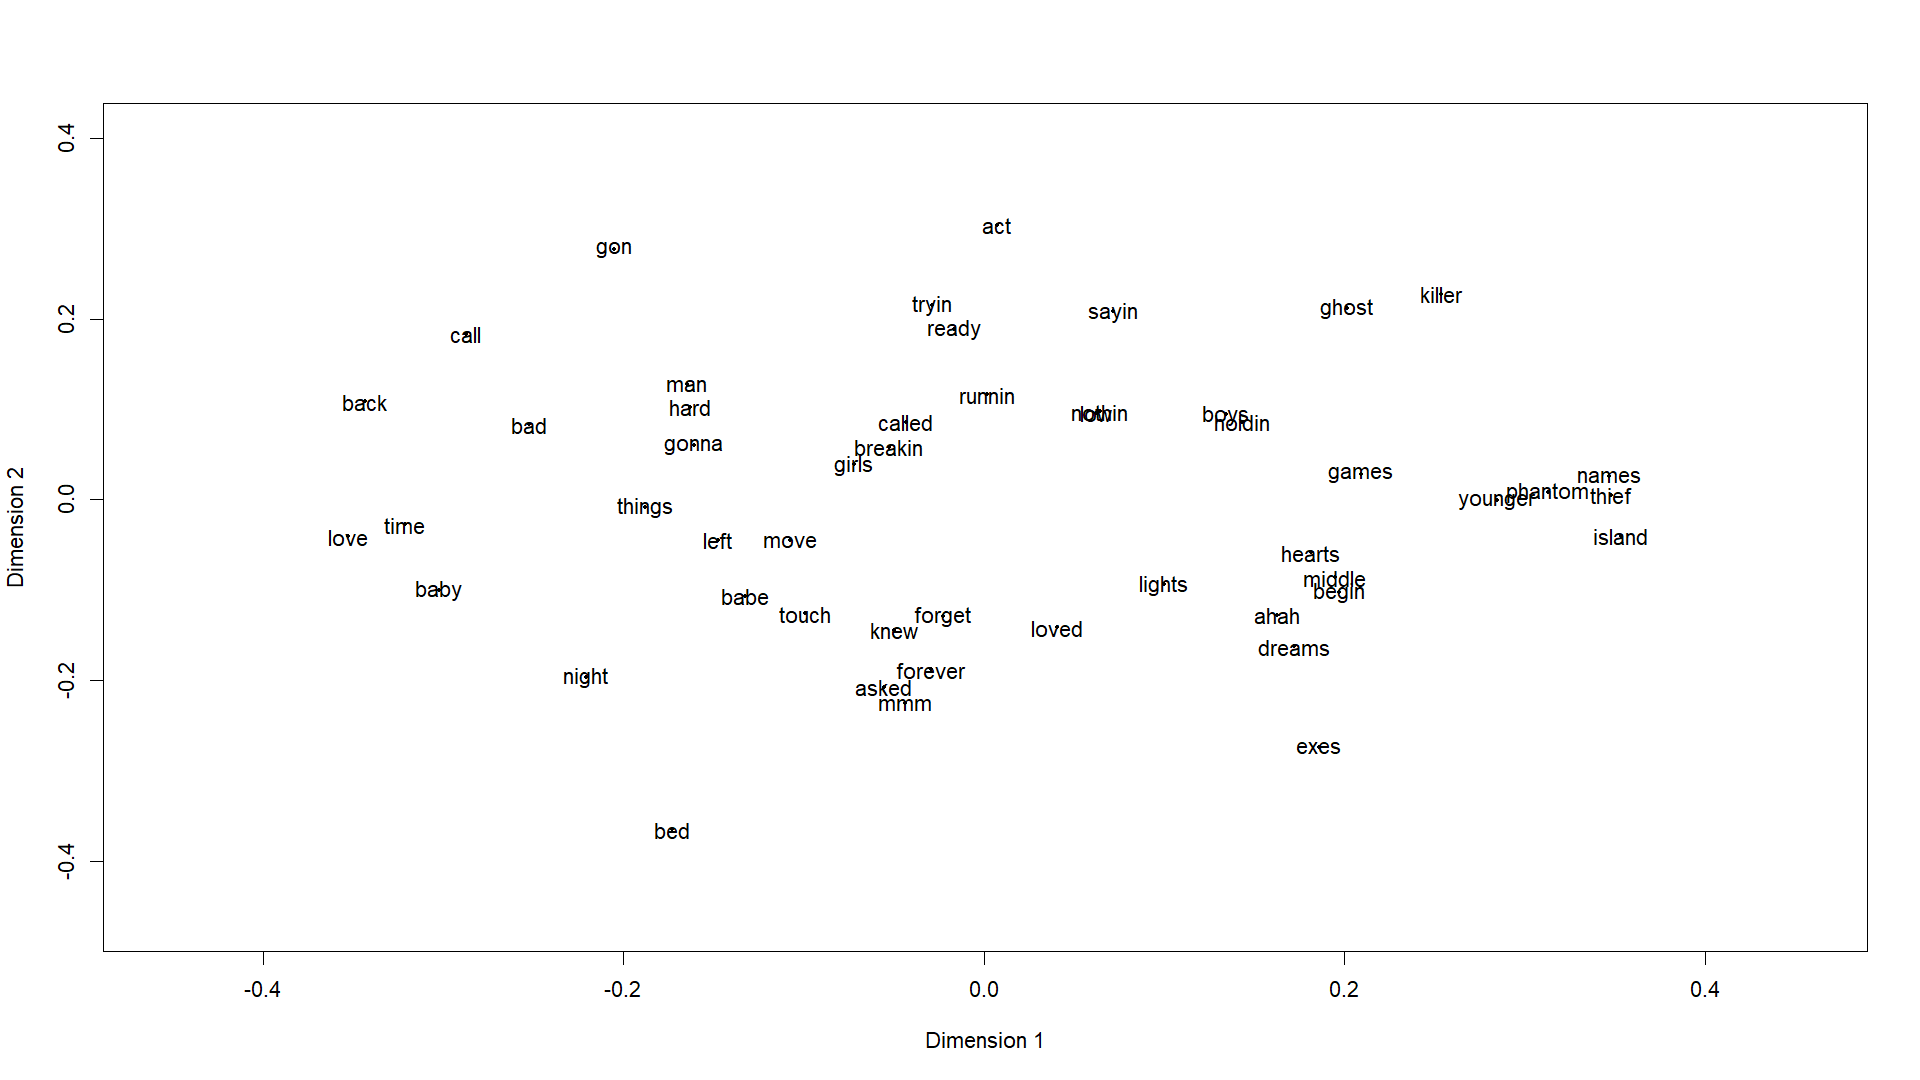
\includegraphics[width=0.8\linewidth]{Images//8_Textual//LSA/first_50_words.png}
    \caption{Primeres 50 paraules en l'MDS de l'LSA traduït}
    \label{fig:textual_lsa_trans_50w}
\end{figure}

\begin{figure}[H]
\centering
    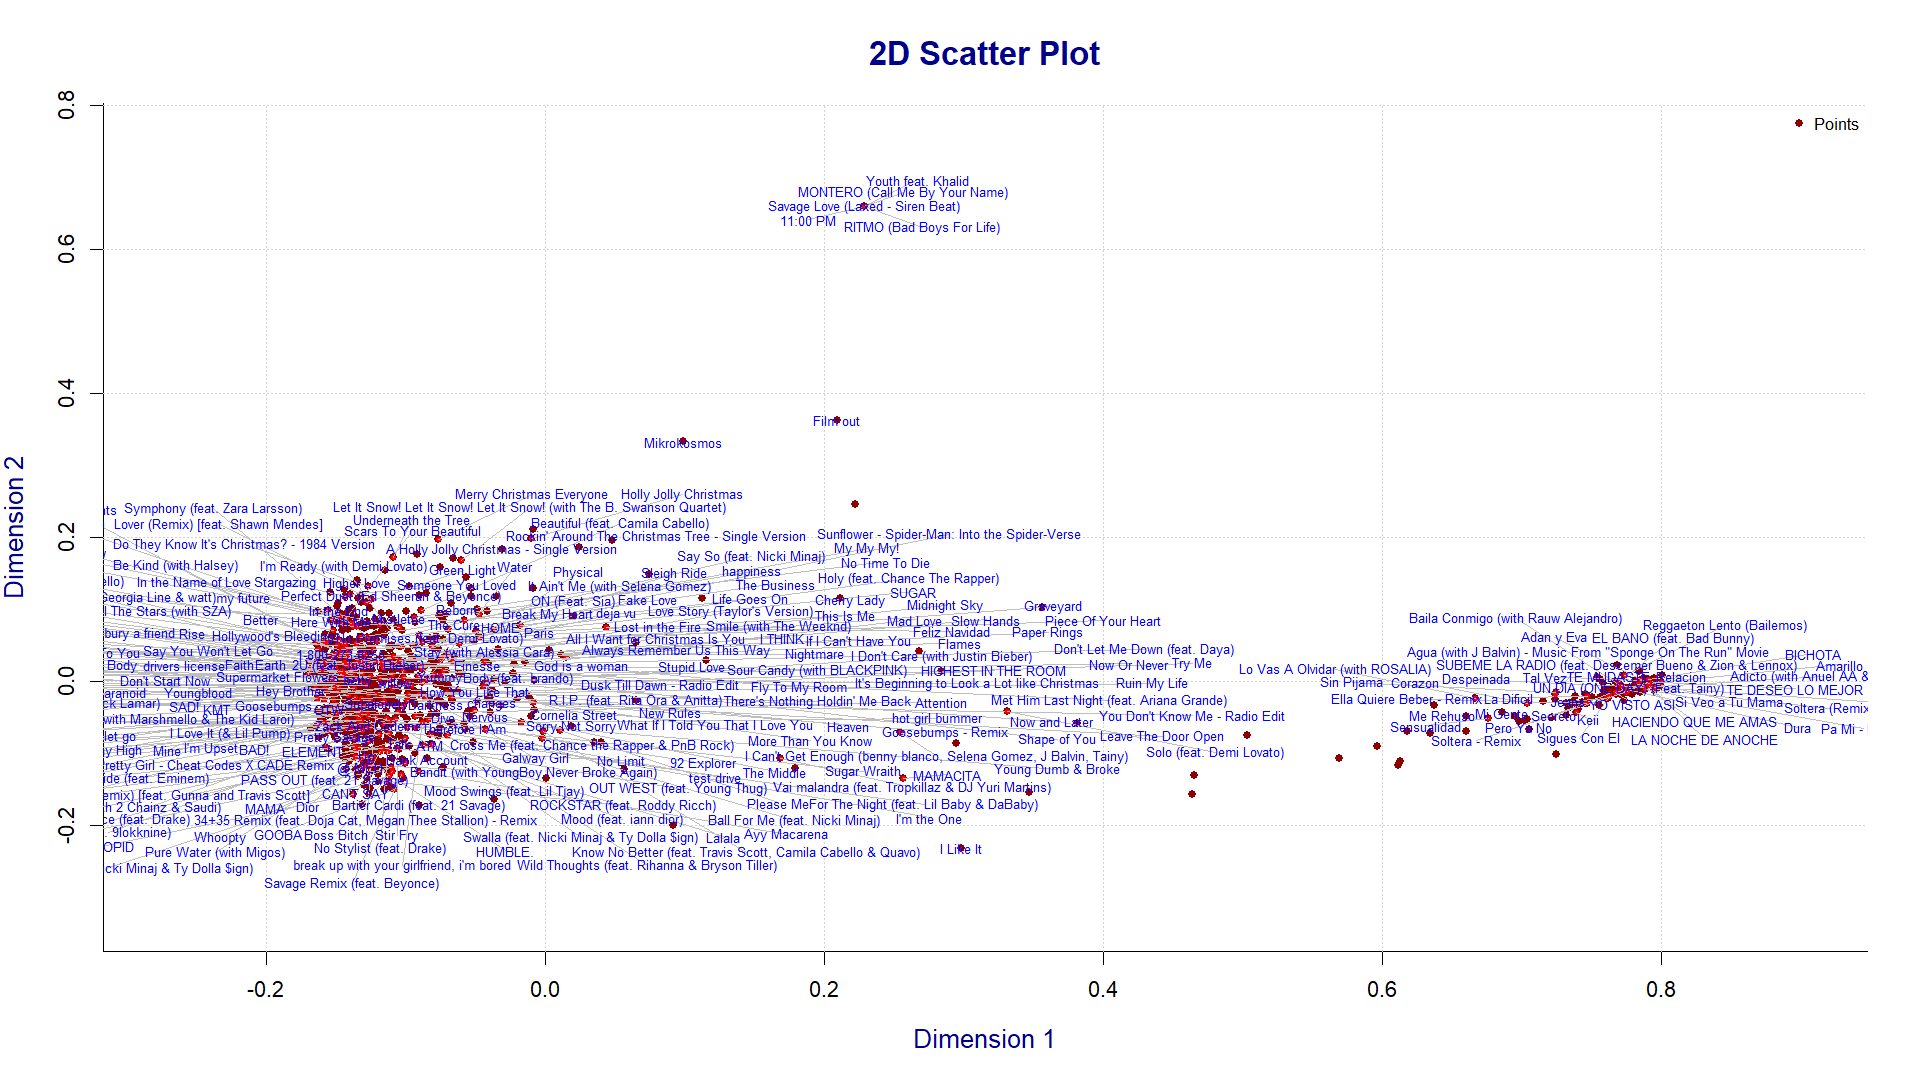
\includegraphics[width=0.8\linewidth]{Images//8_Textual//LSA/orignal_all_songs_MDS.png}
    \caption{Totes les cançons en l'MDS de l'LSA original}
    \label{fig:textual_lsa_original_allsongsMDS}
\end{figure}

\begin{figure}[H]
\centering
    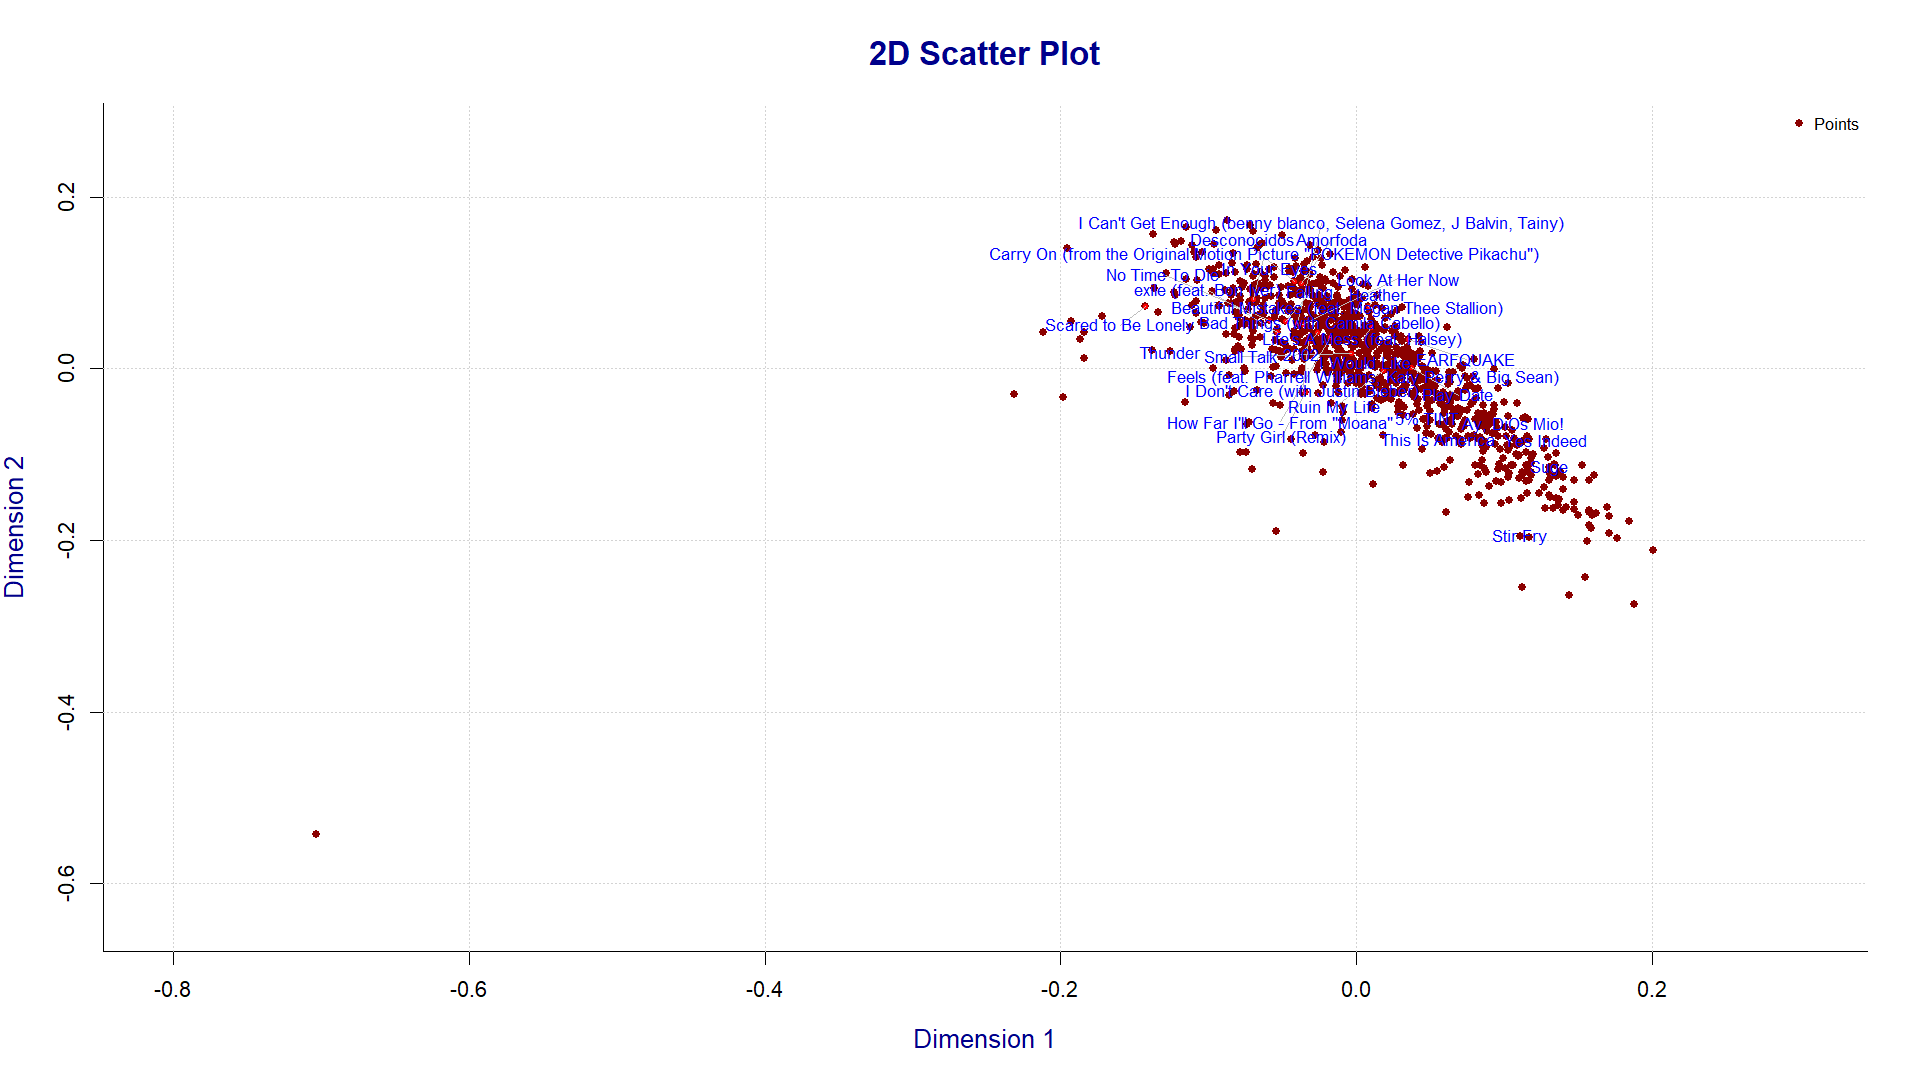
\includegraphics[width=0.8\linewidth]{Images//8_Textual//LSA/all_songs_less_labels_MDS.png}
    \caption{Totes les cançons en l'MDS de l'LSA traduït}
    \label{fig:textual_lsa_trans_allsongsMDS}
\end{figure}

S'observa ja d'entrda com els dos espais son diferents: les primeres 50 paraules són les mateixes, ja que la primera cançó és en anglès, però es distribueixen de forma lleugerament diferent (i els documents encara més).

Es pot veure com \textit{time} esta molt a prop de \textit{love}, però en canvi lluny de paraules com \textit{hard} o \textit{bad}. Tot i això, és complicat interpretar com es distribueixen les paraules en aquest espai.

Pel que fa a les cançons, és més fàcil interpretar el plot. En l'orignal, s'observen 3 grans grups: les cançons en anglès, les que estan en castellà i les que tenen "unknown". En canvi, en la versió traduïda es concentren els grups de l'anglès i el castellà en un de sol.

Podem observar directament els resultats en les dues primeres dimensions de l'LSA (per paraules \ref{fig:textual_lsa_original_default_words} \ref{fig:textual_lsa_trans_default_words} i per documents \ref{fig:textual_lsa_original_default} \ref{fig:textual_lsa_trans_default}):

\begin{figure}[H]
    \centering
    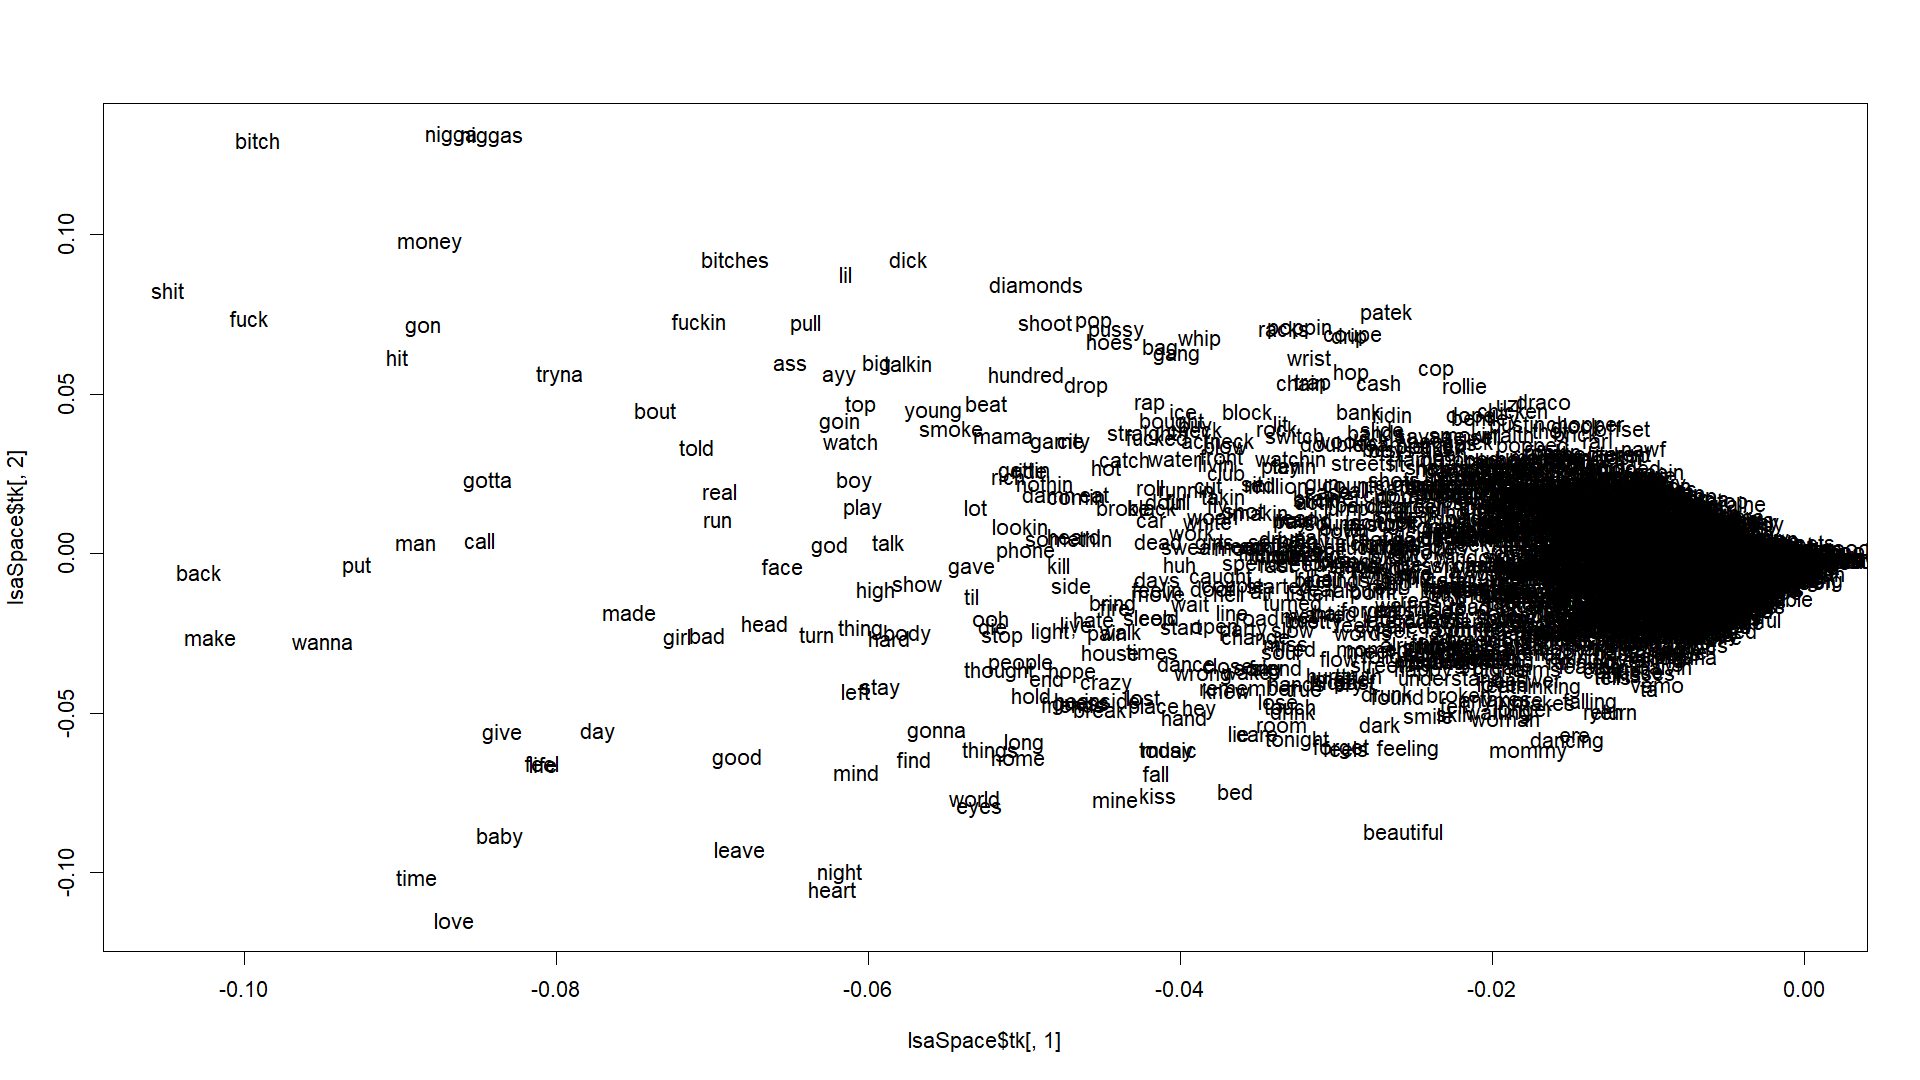
\includegraphics[width=0.8\linewidth]{Images//8_Textual//LSA/lsa_default_space_words.png}
    \caption{Paraules en les dues primeres k de l'LSA original}
    \label{fig:textual_lsa_original_default_words}
\end{figure}

\begin{figure}[H]
    \centering
    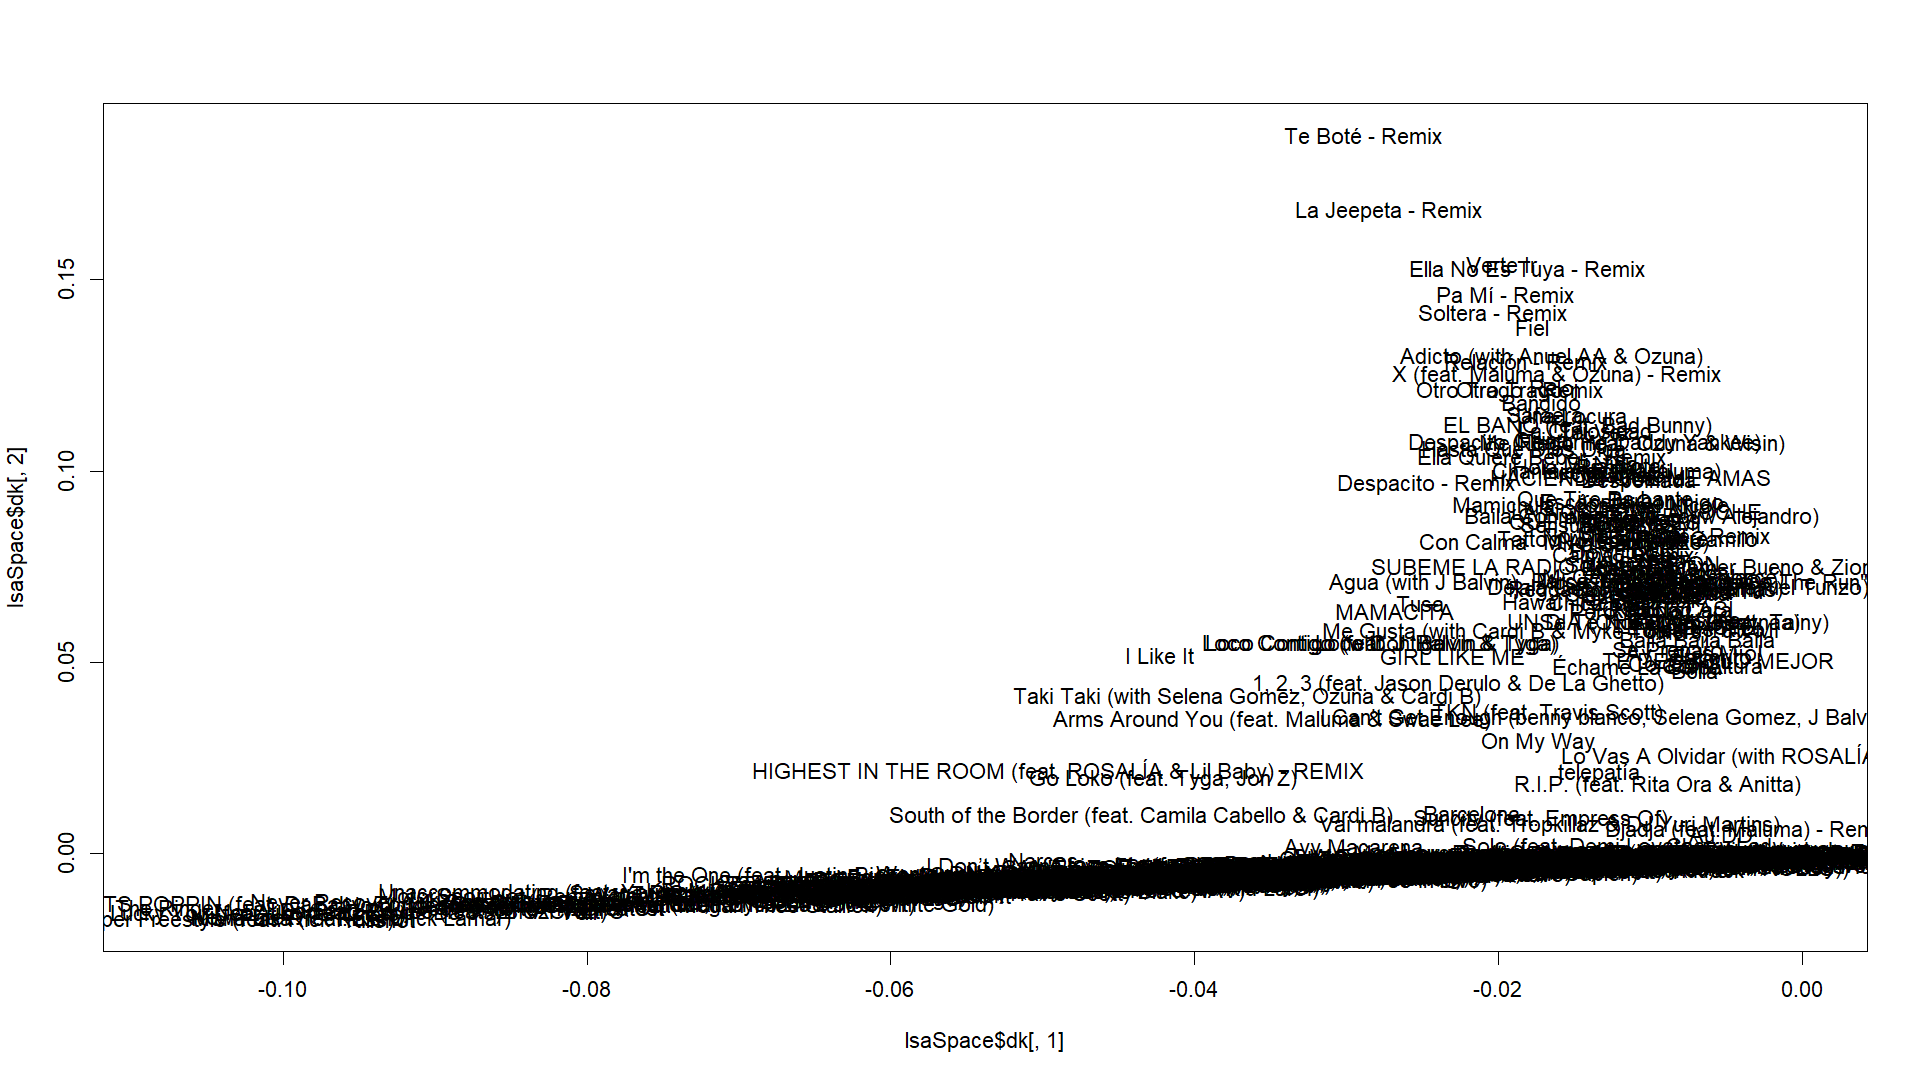
\includegraphics[width=0.8\linewidth]{Images//8_Textual//LSA/original_lsa_default_space.png}
    \caption{Documents en les dues primeres k de l'LSA original}
    \label{fig:textual_lsa_original_default}
\end{figure}

\begin{figure}[H]
    \centering
    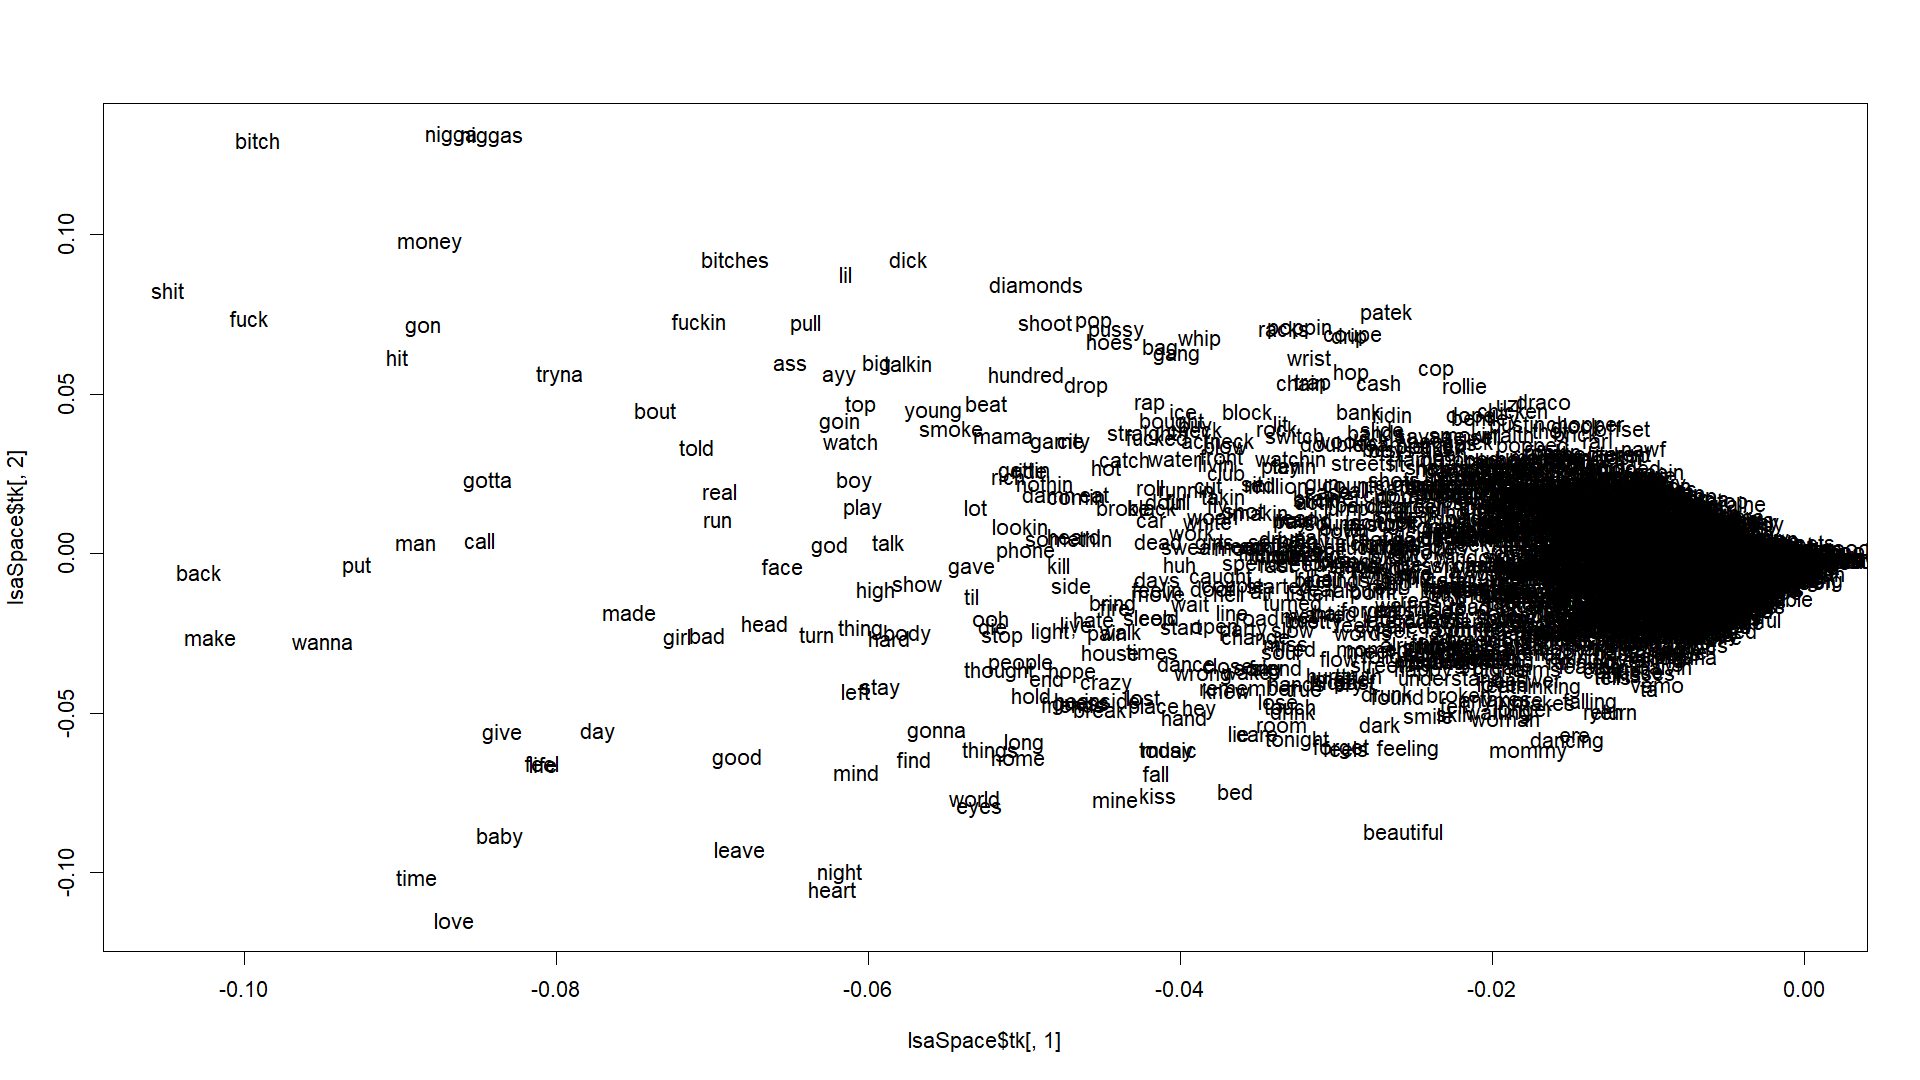
\includegraphics[width=0.8\linewidth]{Images//8_Textual//LSA/lsa_default_space_words.png}
    \caption{Paraules en les dues primeres k de l'LSA traduït}
    \label{fig:textual_lsa_trans_default_words}
\end{figure}

\begin{figure}[H]
    \centering
    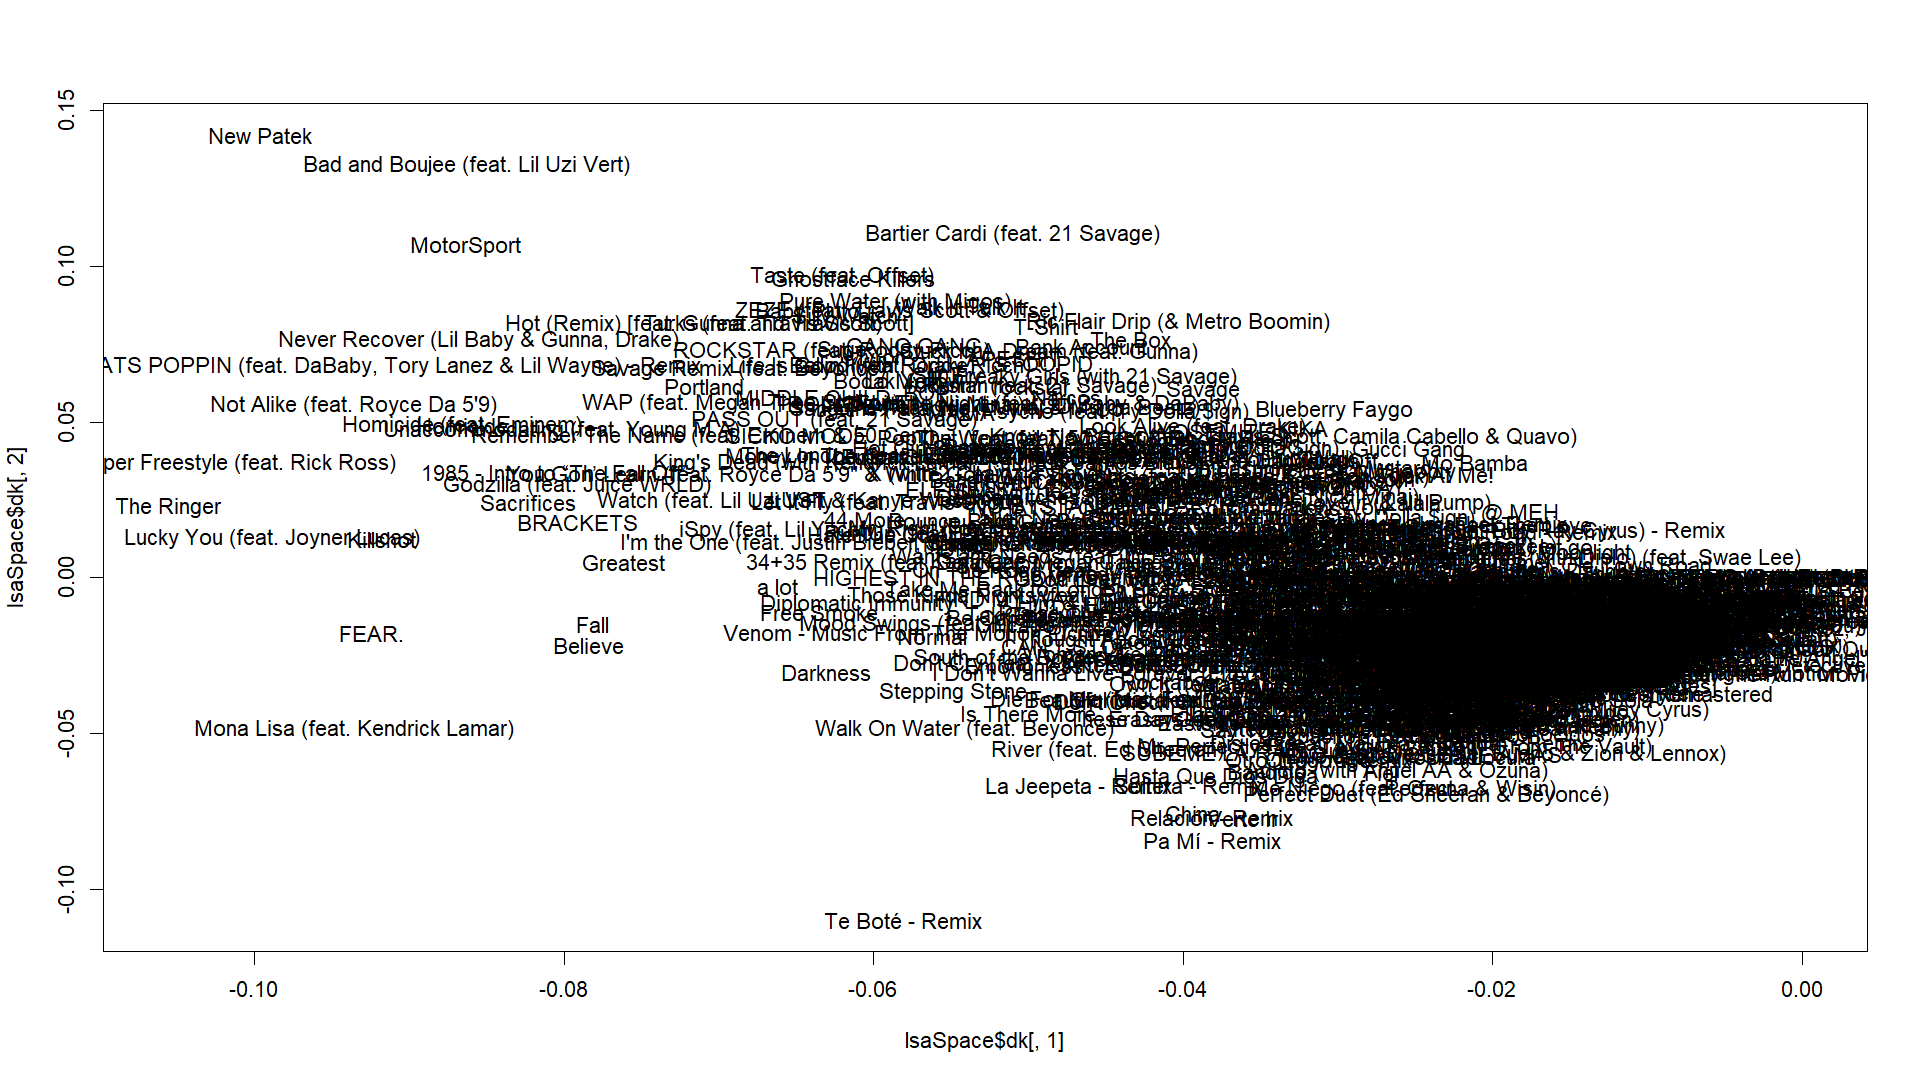
\includegraphics[width=0.8\linewidth]{Images//8_Textual//LSA/lsa_default_space.png}
    \caption{Documents en les dues primeres k de l'LSA traduït}
    \label{fig:textual_lsa_trans_default}
\end{figure}

S'observen alguns patrons interessant. D'entrada, a l'original hi ha una clara diferència entre les paraules en anglès i en castellà, i aquest fet es tradueix també als documents (sembla ser que la k 1, o el primer topic, se centra en diferenciar paraules en anglès, i el segon aquelles en castellà). En les paraules, observem com aquelles paraules que son iguals en anglès i en castellà, o que se solen usar en anglès en les cançons (com baby, flow...) se situen a la bisectriu dels dos grups. Amb els documents, els situats enmig son alguns que combinen part de la lletra en anglès i part en castellà, i a més la separació és encara més marcada.

Pel que fa a l'LSA de les paraules traduïdes, l'eix 1 és complicat d'interpretar, tot i que sembla ser que es refereix a les paraules més usades o comunes en general. L'eix 2 representa en certa manera com de malsonant és una paraula: les que estan situades més amunt (valors més elevats) són insults o paraules dolentes, molts cops associades al hip\_hop, mentre que en la part de baix trobem paraules com amor (\textit{love}) o \textit{beautiful}. Del cúmol de la dreta és complicat dir-ne gaires coses, ja que hi ha moltes paraules juntes i no es poden diferenciar (segurament en alguna altra dimensió sí).

Pel que fa a les cançons, en general cap a l'esquerra i amunt trobem cançons de hip\_hop (especialment dues de Lil Uzi Vert a dalt de tot), mentre que cap al centre i la part de baix sembla haver-hi cançons de reggaeton. Tot i això, altre cop és complicat d'interpretar degut a la gran quantitat d'etiquetes.

Podem observar les paraules que influeixen en els primers topics (ks):

\begin{figure}[H]
    \centering
    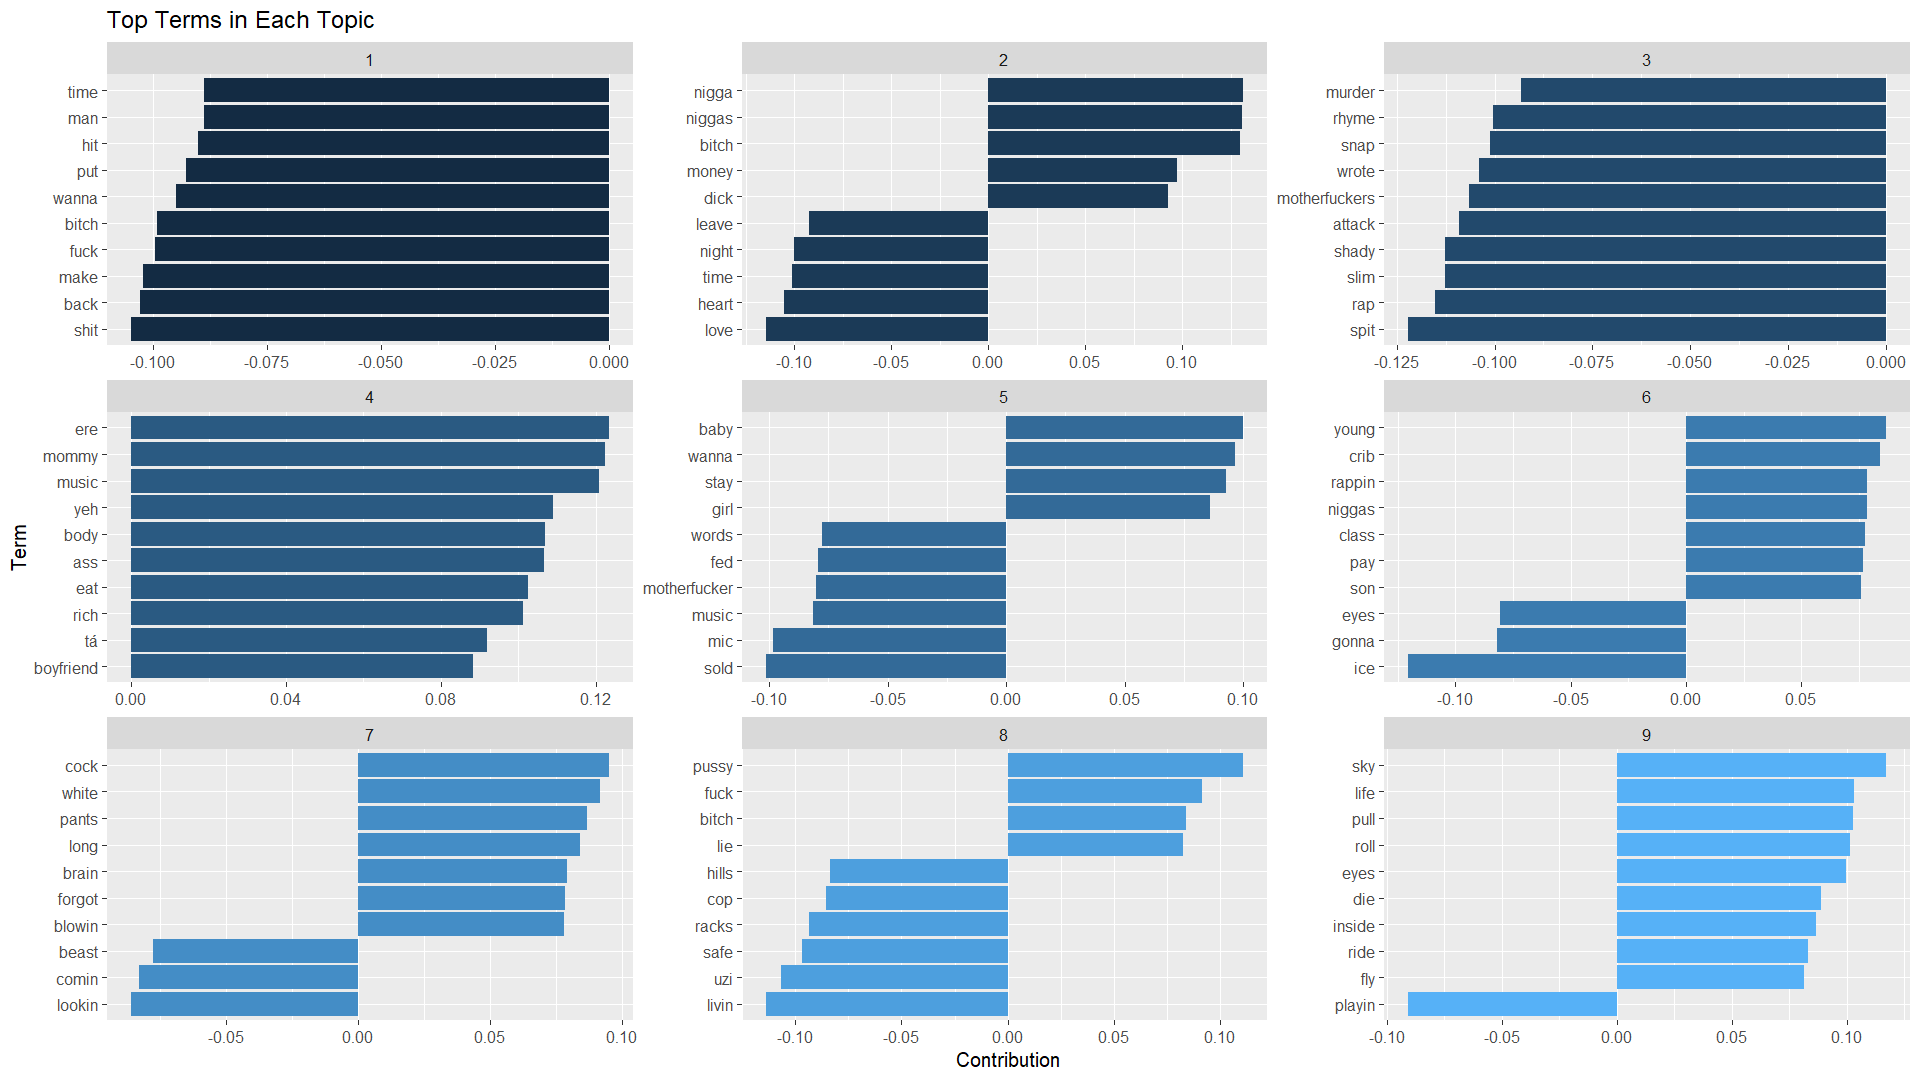
\includegraphics[width=0.8\linewidth]{Images//8_Textual//LSA/lsa_topics_1_9.png}
    \caption{Primers 9 topics de l'LSA traduït}
    \label{fig:textual_lsa_topics9}
\end{figure}

És complicat analitzer els significats de cada topic, ja que molts repeteixen paraules. Tot i això, sembla ser que el primer li influència negativament parlar del temps, homes, o insultar (llavors probablement tingui valors positius cançons simples i no explícites); el segon com hem comentat té paraules malsonants d'una banda i amor de l'altra; el tercer tracta sobre temes violents; el quart i el cinquè sobre sexuals o parelles, el sisè sobre rap...

En total n'hi ha molts, i no es poden interpretar tots. Més endavant realitzarem l'LDA que obtindrà uns millors topics.


Per visualitzar lleugerament les relacions entre documents també s'ha usat la matriu de distàncies en aquest espai LSA, per realitzar un MDS i plotejar els resultats (i s'ha limitat el nombre d'etiquetes). Observem les figures \ref{fig:textual_lsa_dist_orig} i \ref{fig:textual_lsa_dist_trad}.

\begin{figure}[H]
    \centering
    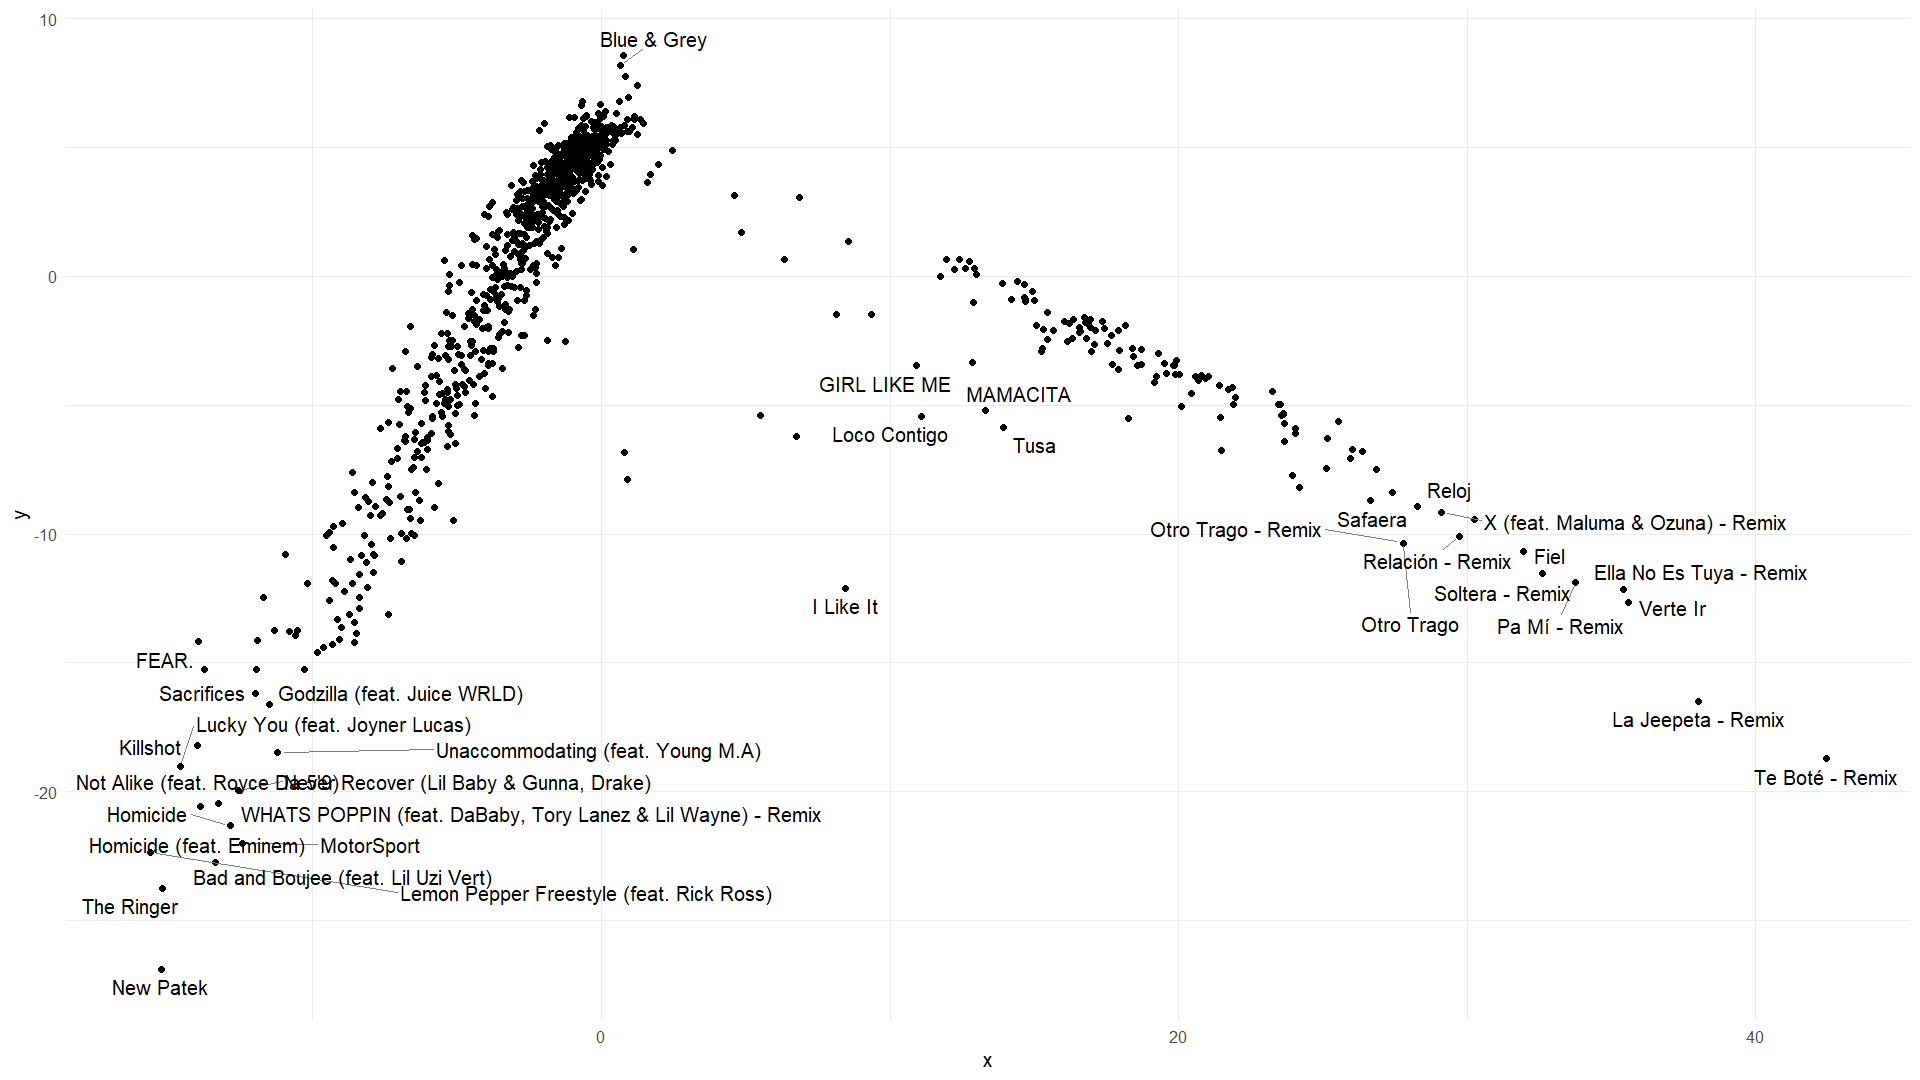
\includegraphics[width=0.8\linewidth]{Images//8_Textual//LSA/original_distances_outliers.png}
    \caption{Representació documents LSA original}
    \label{fig:textual_lsa_dist_orig}
\end{figure}

\begin{figure}[H]
    \centering
    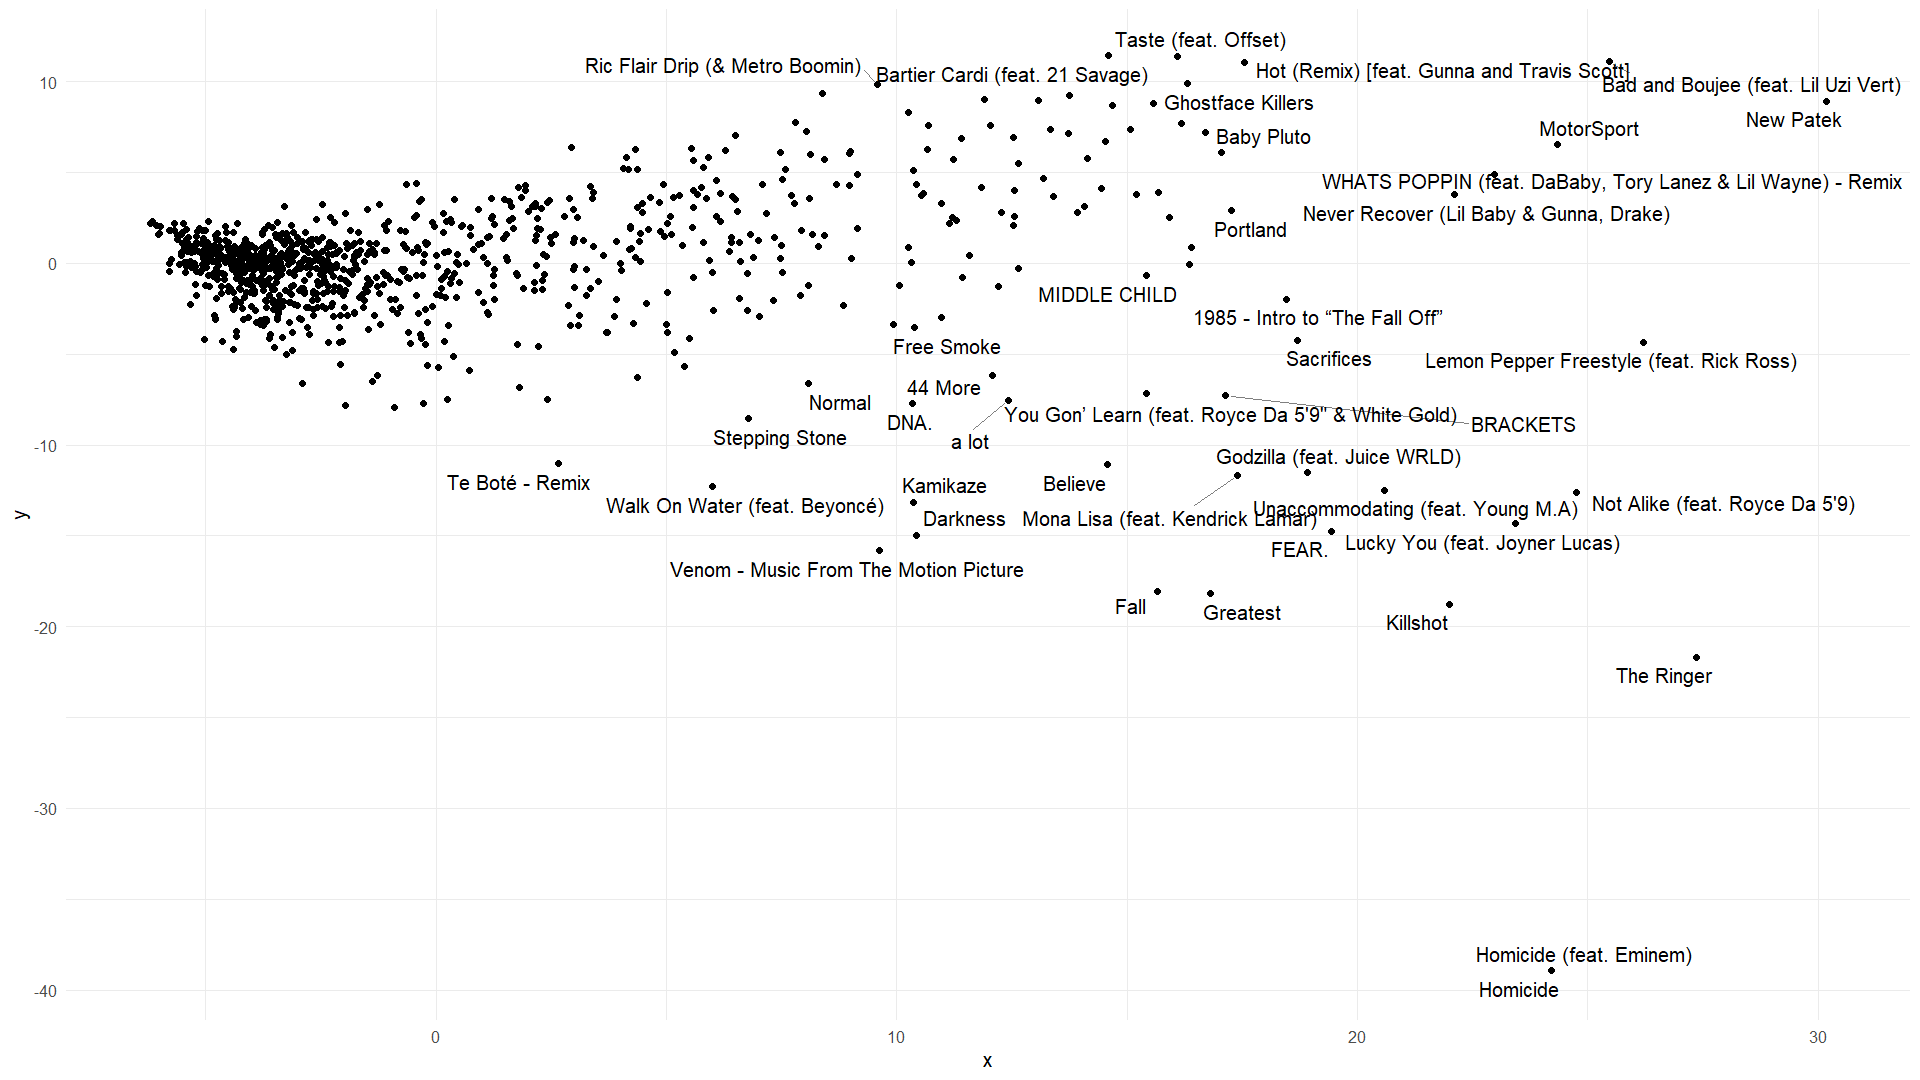
\includegraphics[width=0.8\linewidth]{Images//8_Textual//LSA/distances_outliers.png}
    \caption{Representació documents LSA traduït}
    \label{fig:textual_lsa_dist_trad}
\end{figure}

En l'original, observem dos grups en forma de V invertida: a l'esquerra, el més nombros, que conté cançons en anglès: a la dreta, cançons en castellà. Els punts que estan més elevats (on apareix \textit{Blue and Grey}) són cançons de K-pop (parts en anglès, però també parts en coreà). Com més avall estan les cançons, més llargues són les seves lletres (les d'anglès son cançons de rap amb moltes paraules, i les de castellà més llargues són remixos, que també solen afegir estrofes i són més llargues que les normals). 

En la versió traduïda, és més complicat trobar una explicació a la distribució. En general, els punts que estan més dispersos (i que per tant s'han pogut etiquetar) són cançons de rap o hip hop. A part d'això, d'entrada no sembla haver-hi cap relació considerable com en l'anterior.

Com que tenim més informació sobre cada document, podem pintar els punts de colors. Per exemple, observarem la distribució de latino \ref{fig:textual_lsa_orig_latino} \ref{fig:textual_lsa_trad_latino} i de hip hop \ref{fig:textual_lsa_orig_hiphop} \ref{fig:textual_lsa_trad_hiphop}, que semblen ser els dos gèneres que més destaquen.


\begin{figure}[H]
\centering
    \begin{minipage}{.5\textwidth}
        \centering
        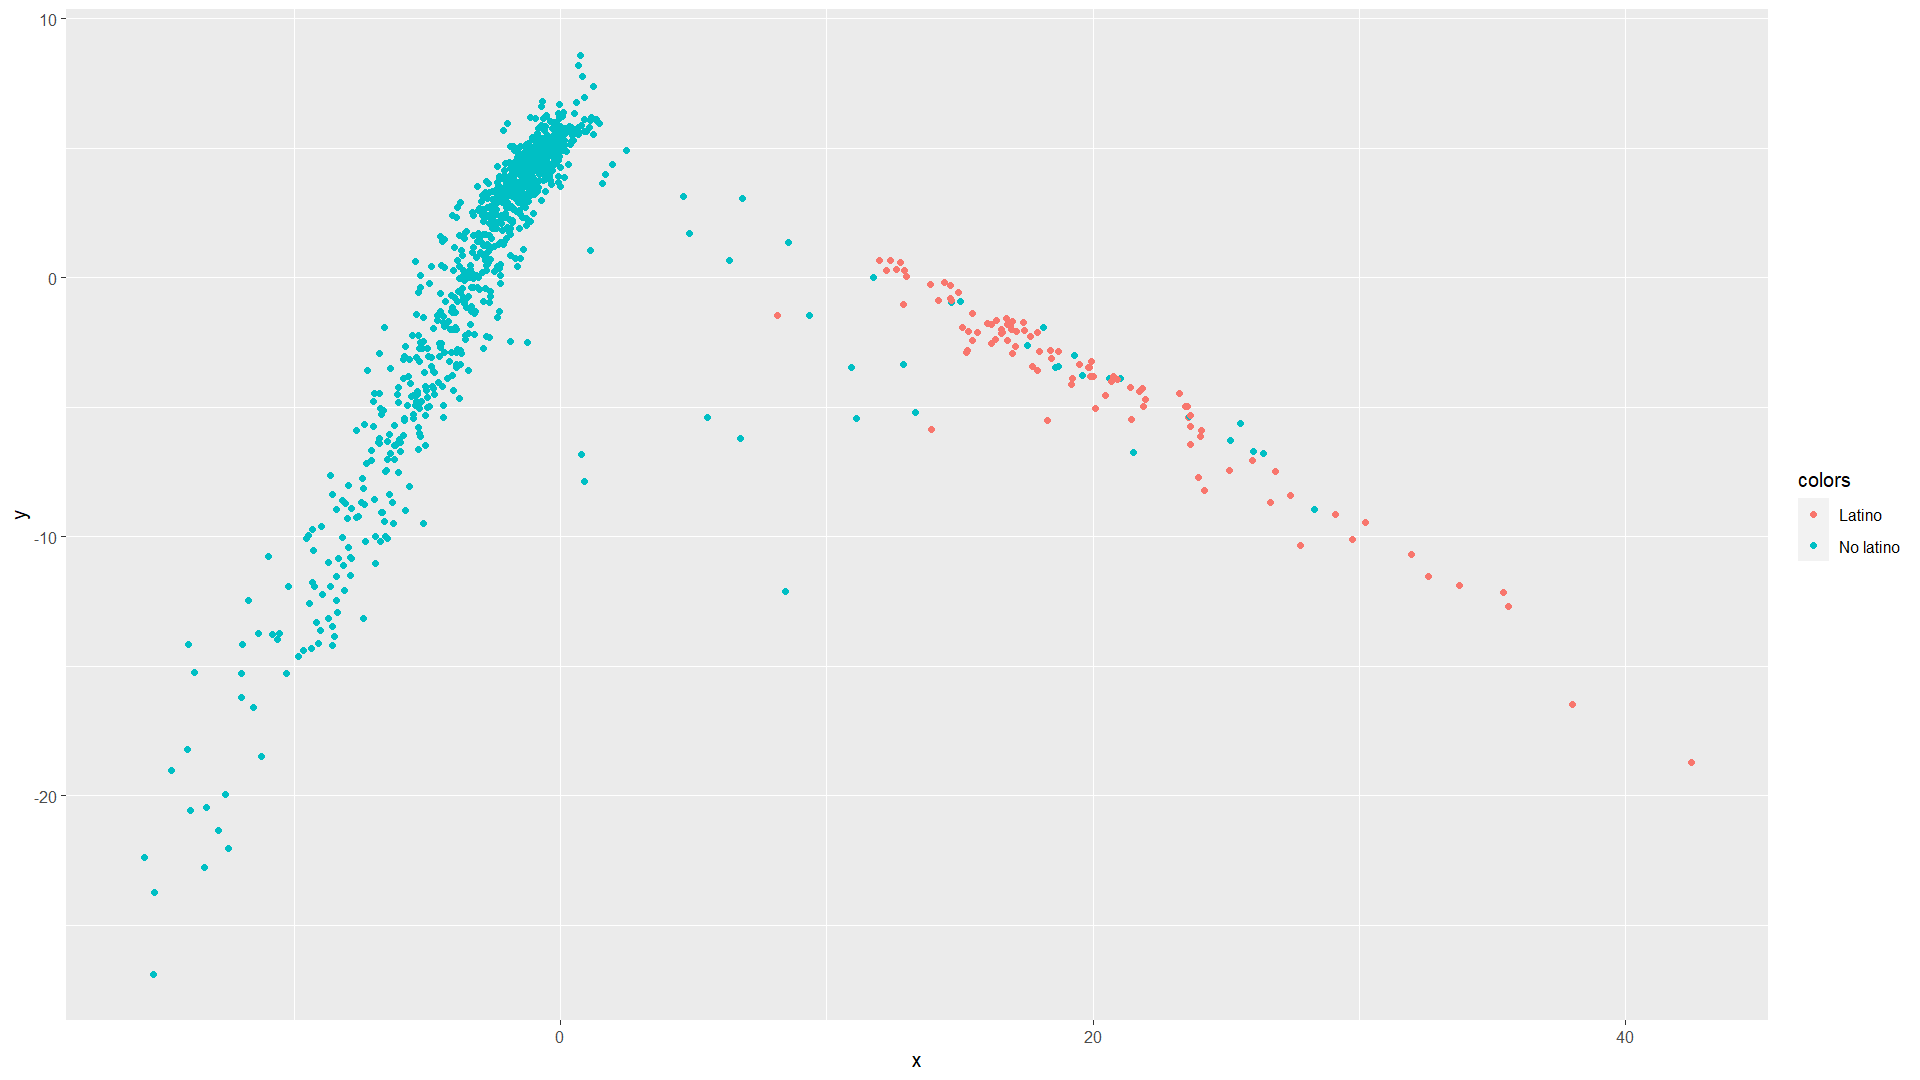
\includegraphics[width=0.95\linewidth]{Images//8_Textual//LSA/original_distances_latino.png}
    \caption{Documents en LSA original, pintats en funció de latino}
    \label{fig:textual_lsa_orig_latino}
    \end{minipage}%
    \begin{minipage}{.5\textwidth}
        \centering
        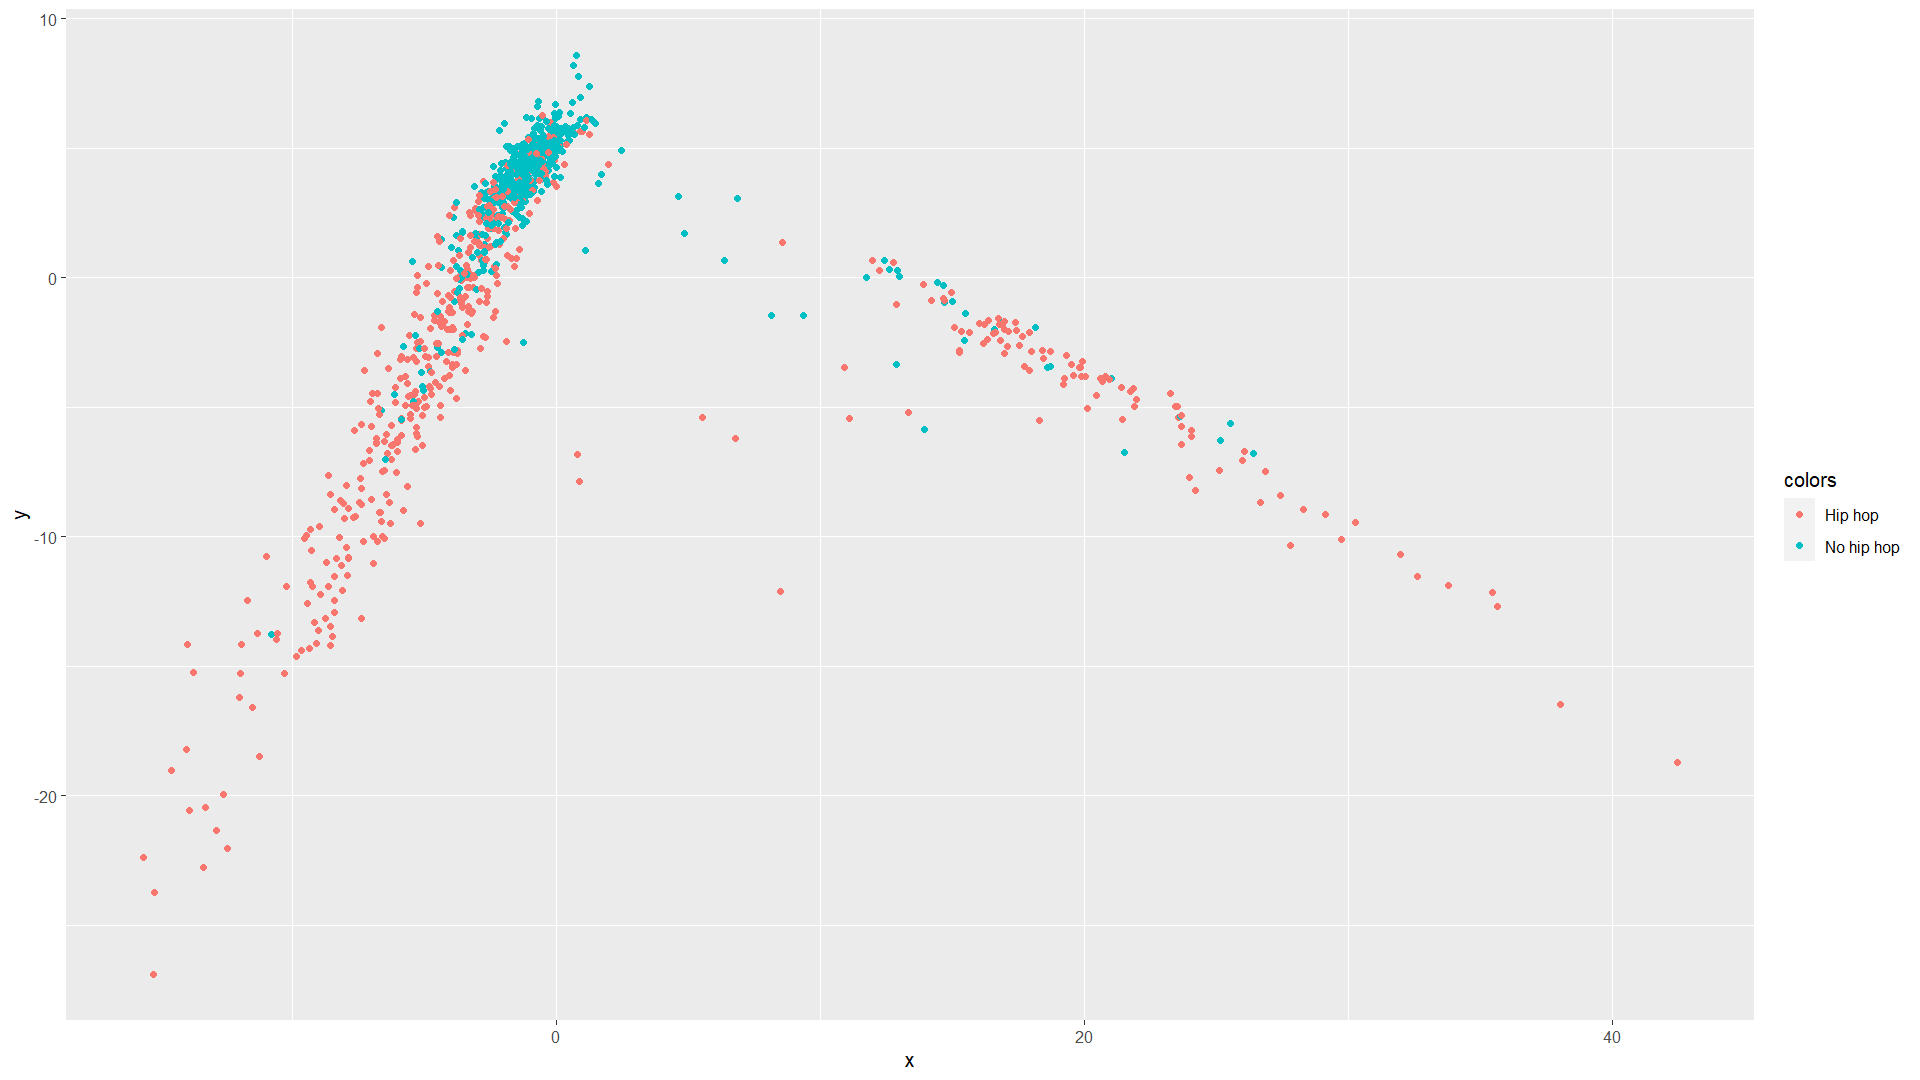
\includegraphics[width=0.95\linewidth]{Images//8_Textual//LSA/original_distances_hip_hop.png}
    \caption{Documents en LSA original, pintats en funció de hip hop}
    \label{fig:textual_lsa_orig_hiphop}
    \end{minipage}%
\end{figure}


\begin{figure}[H]
\centering
    \begin{minipage}{.5\textwidth}
        \centering
        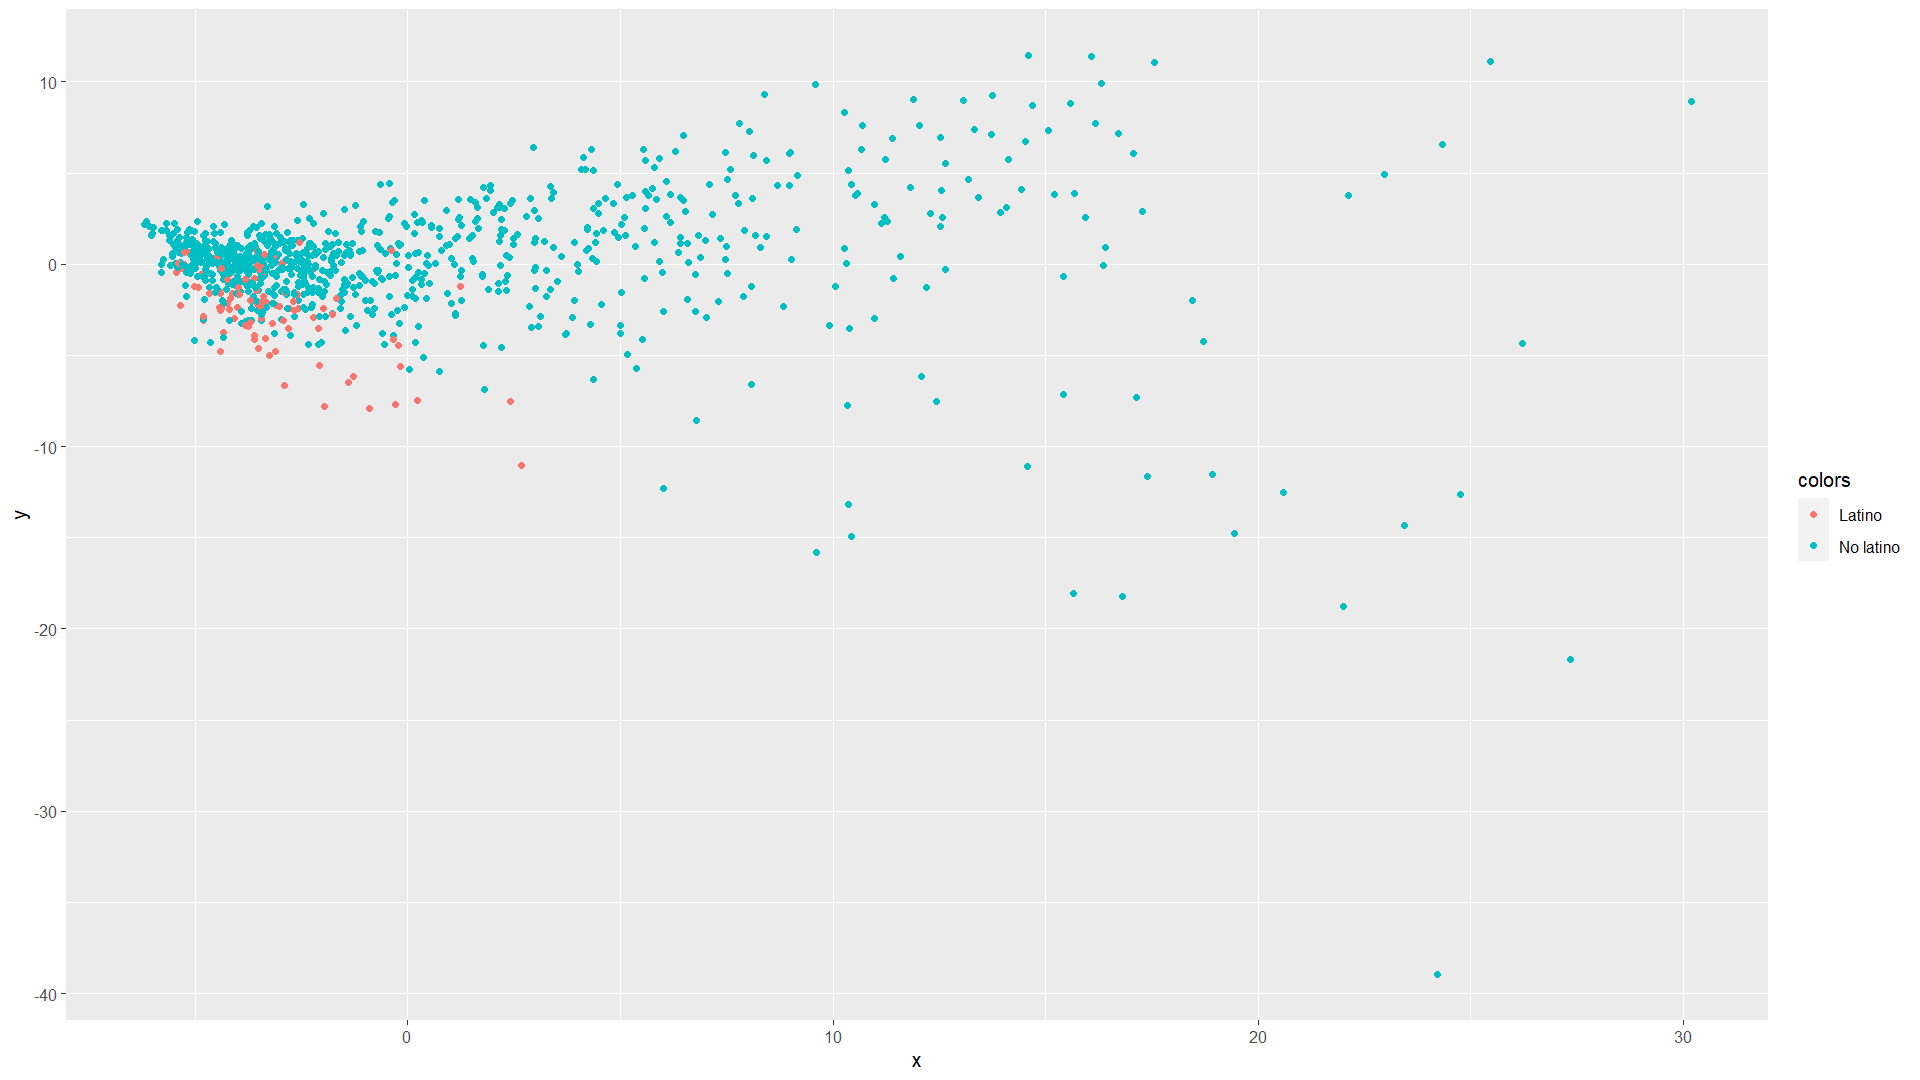
\includegraphics[width=0.95\linewidth]{Images//8_Textual//LSA/distances_latino.png}
    \caption{Documents en LSA traduit, pintats en funció de latino}
    \label{fig:textual_lsa_trad_latino}
    \end{minipage}%
    \begin{minipage}{.5\textwidth}
        \centering
        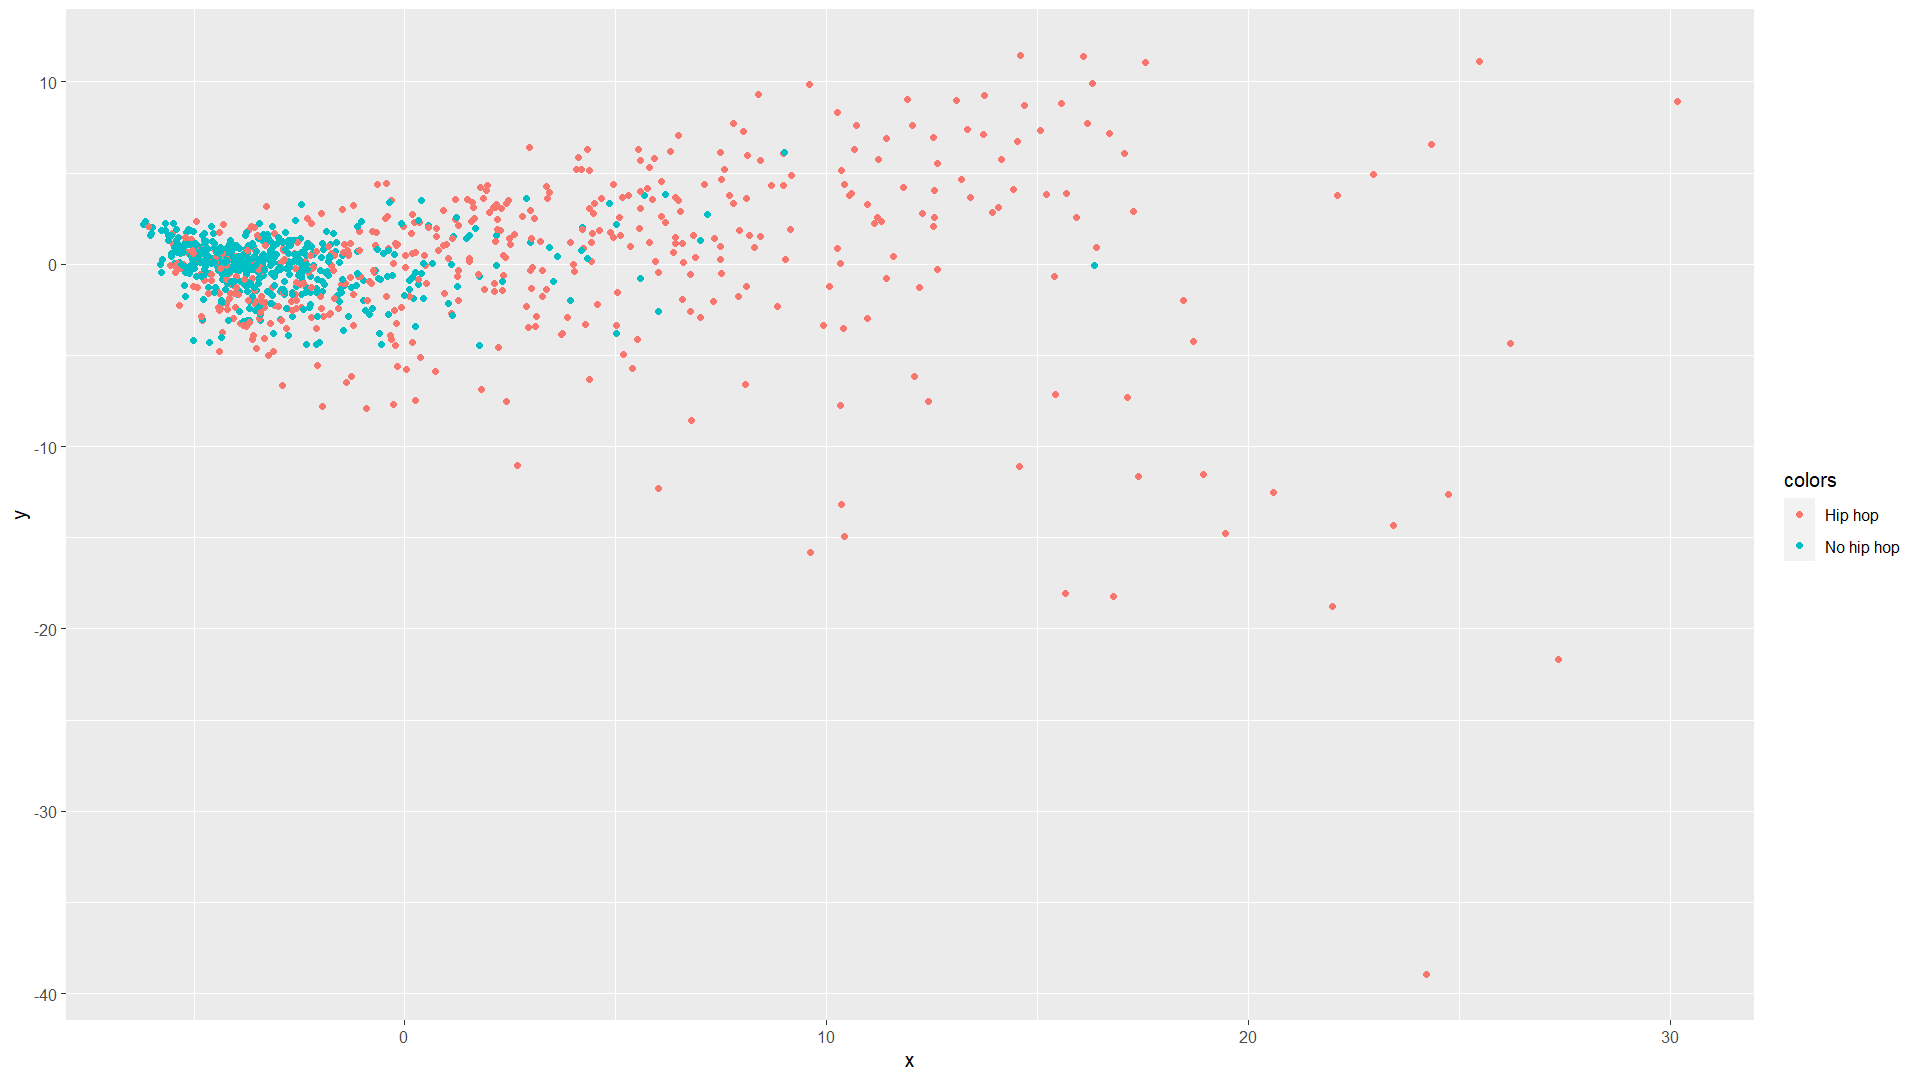
\includegraphics[width=0.95\linewidth]{Images//8_Textual//LSA/distances_hip_hop.png}
    \caption{Documents en LSA traduit, pintats en funció de hip hop}
    \label{fig:textual_lsa_trad_hiphop}
    \end{minipage}%
\end{figure}

Observem com, en l'original, la majoria de cançons que haviem detectat que eren en castellà pertanyen al gènere latino i es situen en aquella diagonal, mentre que no n'hi ha cap en l'altre grup. Pel que fa a hip hop, es distribueixen sobretot en valors petits de la dimensió y. En el traduït també veiem com efectivament els punts dispersos eren cançons de hip hop, i també s'observa com les cançons de latino, tot i estar dins el grup més compacte, se situen més o menys juntes a la part baixa (probablement tractin la majoria de temes similars, o usin paraules semblants).

\subsubsection{Clústering}

En aquest espai, com que les distàncies ens indiquen en certa manera la similitud, es pot també realitzar un clústering, i és una de les coses que s'ha dut a terme. Es poden observar els resultats a les figures


\begin{figure}[H]
    \centering
    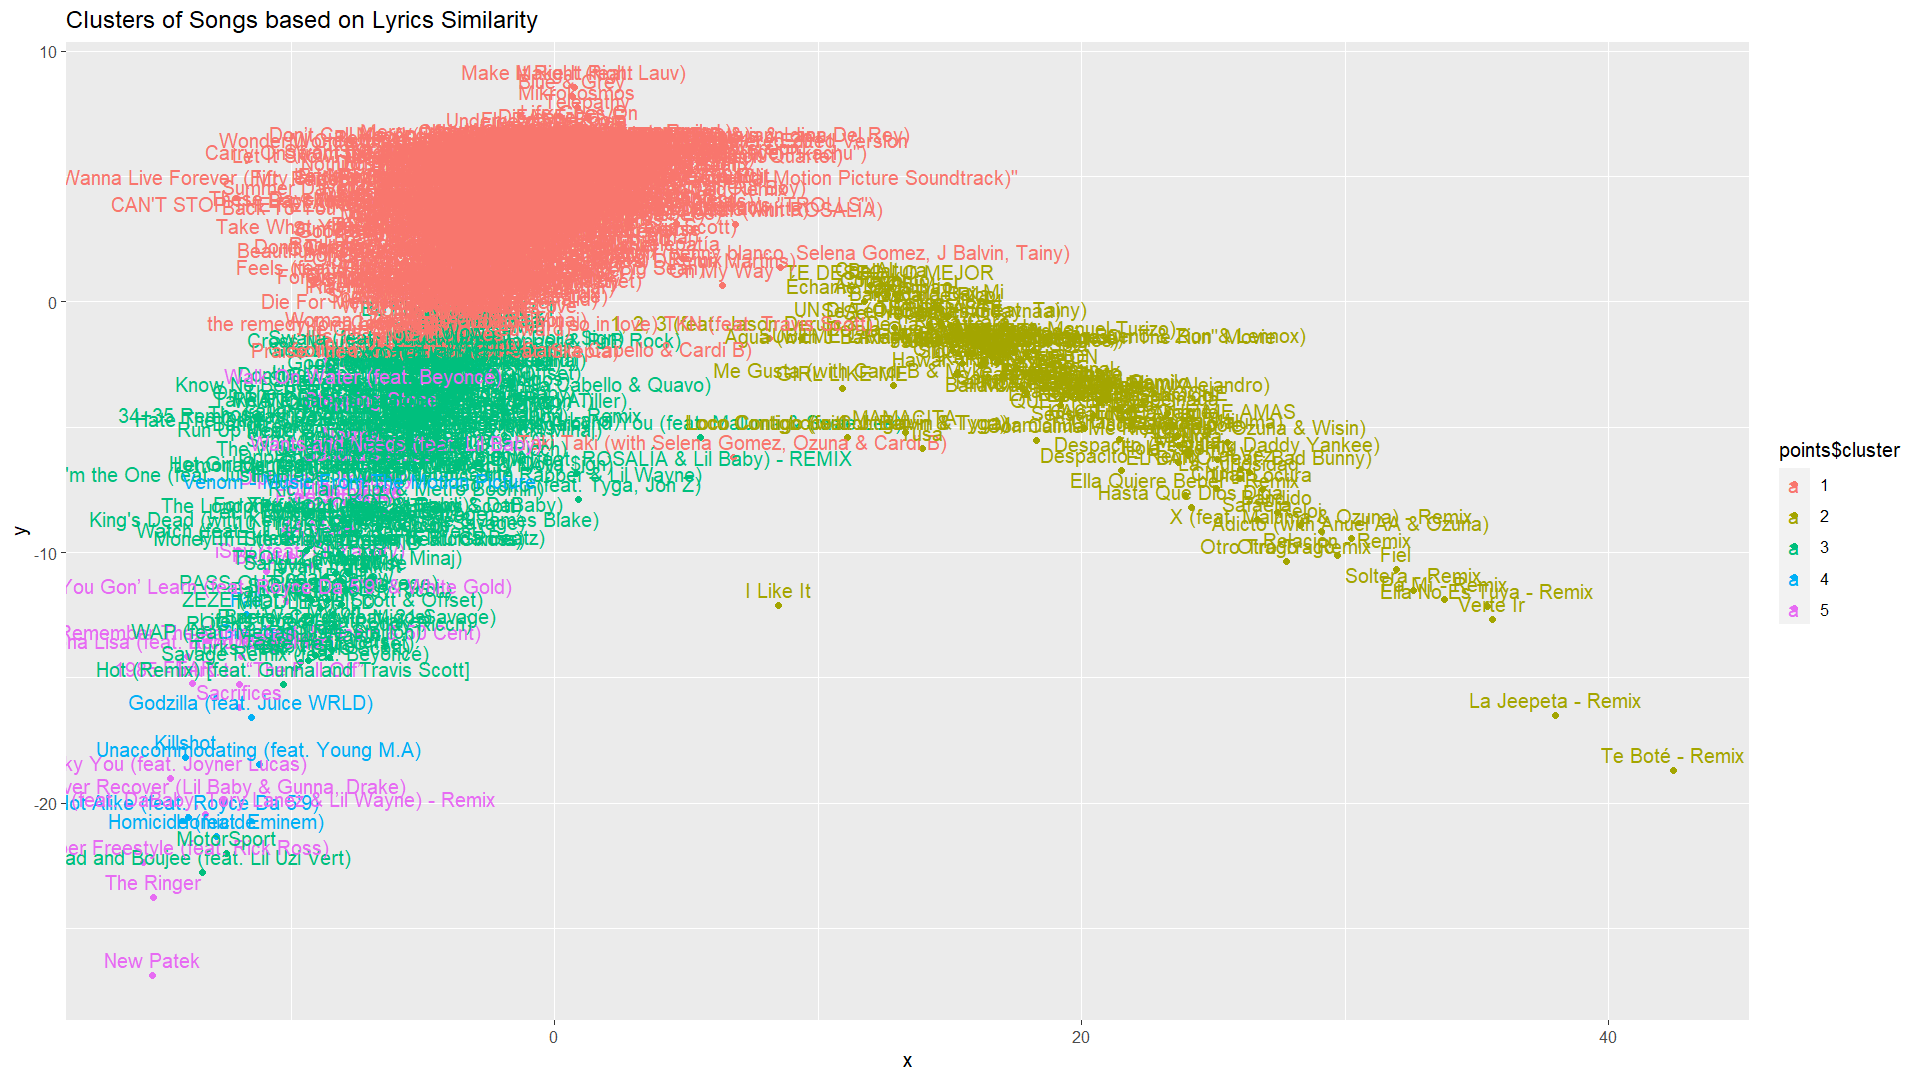
\includegraphics[width=0.8\linewidth]{Images//8_Textual//LSA/original_kmeans_clustering.png}
    \caption{Resultats clústering LSA original}
    \label{fig:textual_lsa_clustering_orig}
\end{figure}

\begin{figure}[H]
    \centering
    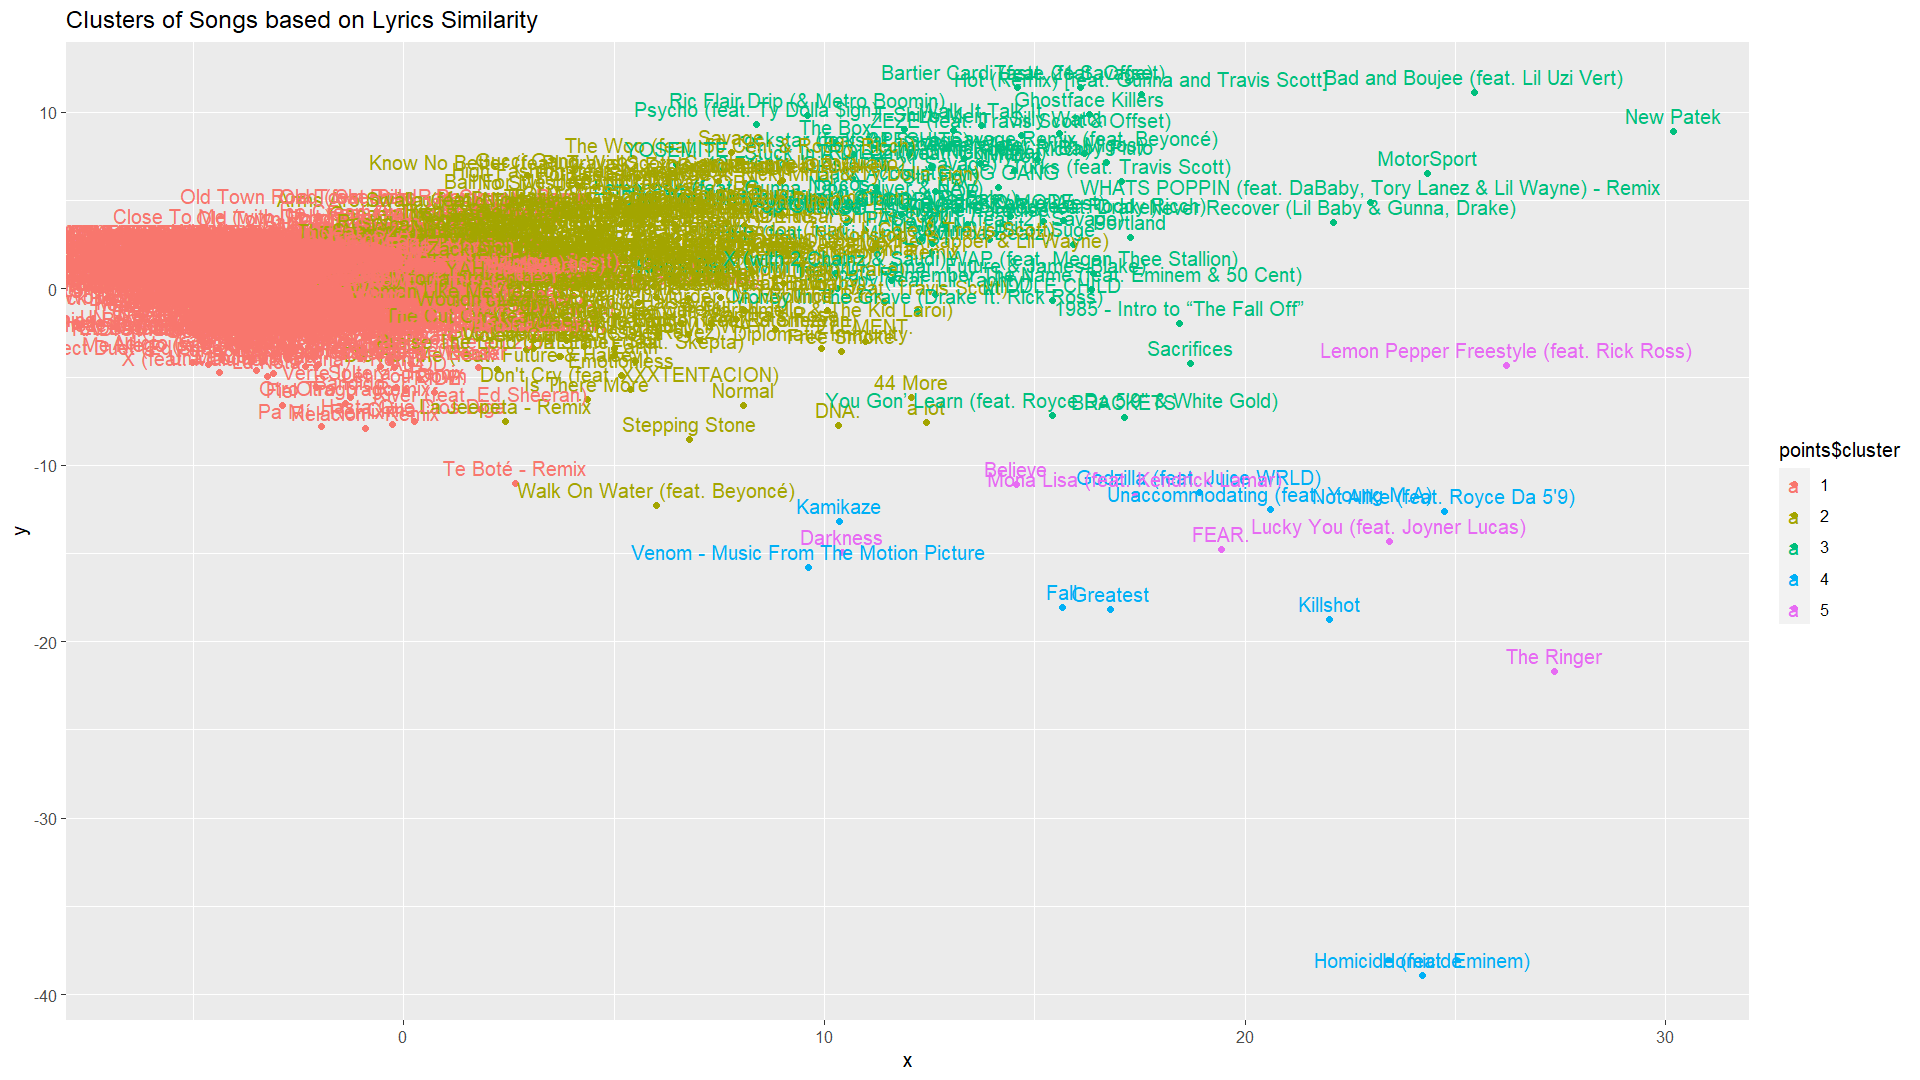
\includegraphics[width=0.8\linewidth]{Images//8_Textual//LSA/kmeans_clustering.png}
    \caption{Resultats clústering LSA traduit}
    \label{fig:textual_lsa_clustering_trad}
\end{figure}

Concretament, s'ha usat un K-means amb k = 5, ja que s'ha considerat que era adequada. En l'original, observem uns grups que es poden diferenciar bastant a simple vista: el clúster 1 engloba aquelles cançons sobretot de pop, el 2 les de latino (reggaeton sobretot), el 3 les de hip hop, el 4 les de Eminem i finalment el 5 més de hip hop però tirant a rap o trap.

En el traduït és lleugerament més complicat. Torna a haver-hi un clúster específic per l'Eminem (el 4), i un altre de cançons de rap (el 5), però els altres 3 són complicats de diferenciar. Per això, s'ha realitzat un petit profiling:

\begin{figure}[H]
    \centering
    \begin{minipage}{.4\textwidth}
        \centering
        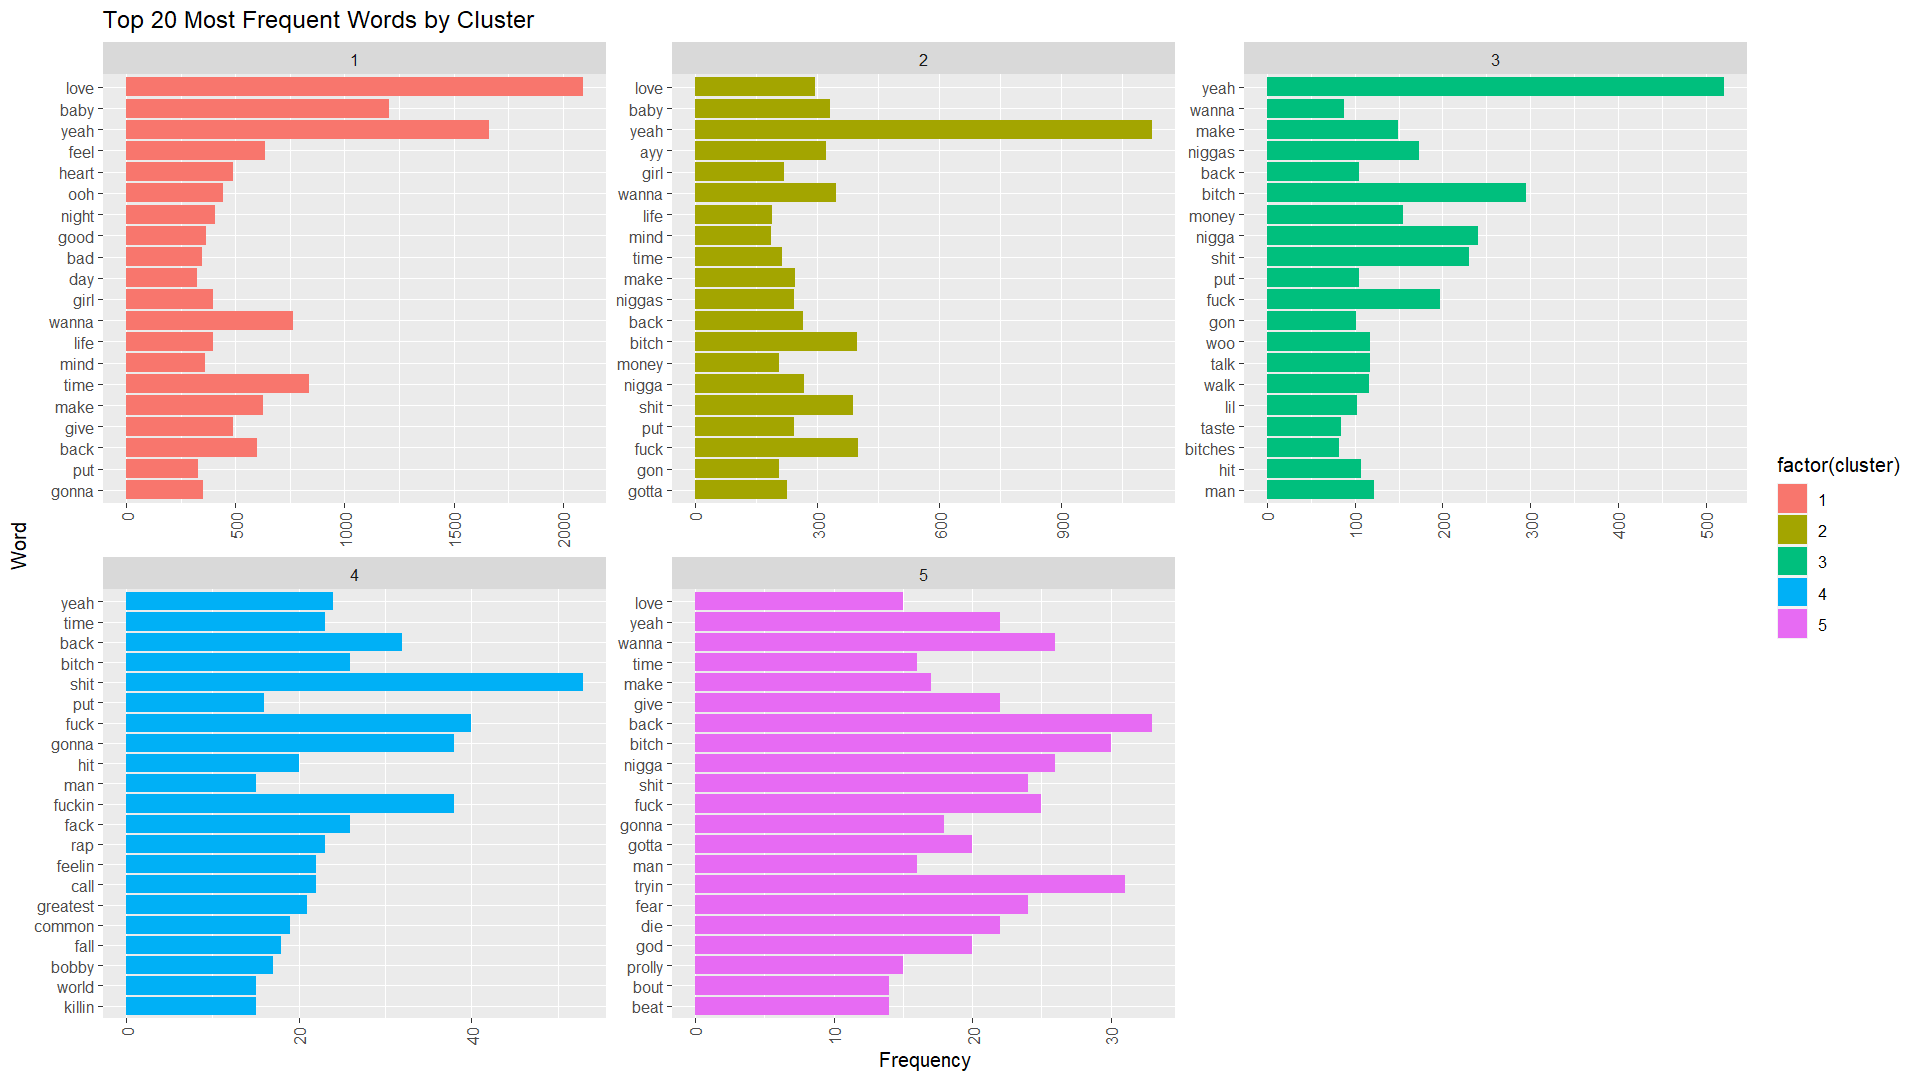
\includegraphics[width=1\linewidth]{Images//8_Textual//LSA/profiling_words_cluster.png}
        \caption{Paraules més utilitzades per clúster}
        \label{fig:textual_lsa_profiling_words}
    \end{minipage}%
    \begin{minipage}{.4\textwidth}
        \centering
        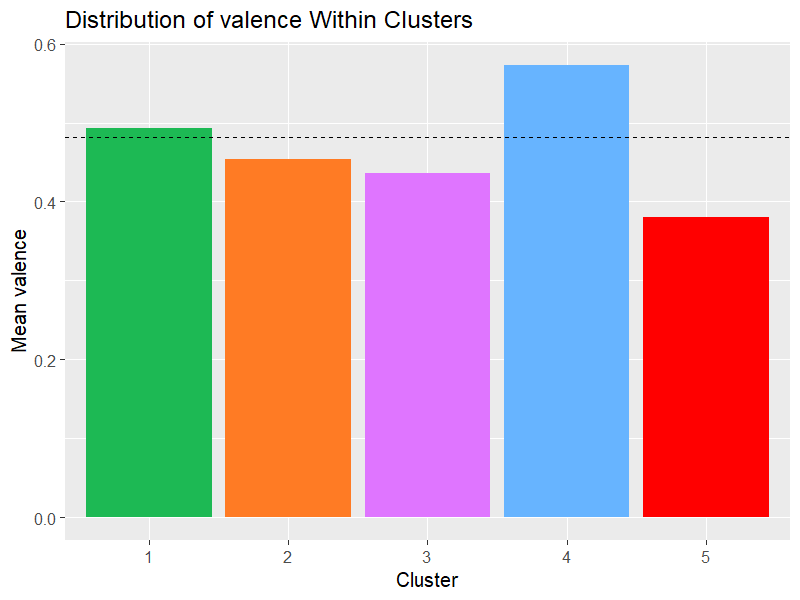
\includegraphics[width=0.95\linewidth]{Images//8_Textual//LSA/profiling_valence.png}
        \caption{Positivitat musical per clúster}
        \label{fig:textual_lsa_profiling_val}
    \end{minipage}%
\end{figure}

\begin{figure}[H]
    \centering
    \begin{minipage}{.4\textwidth}
        \centering
        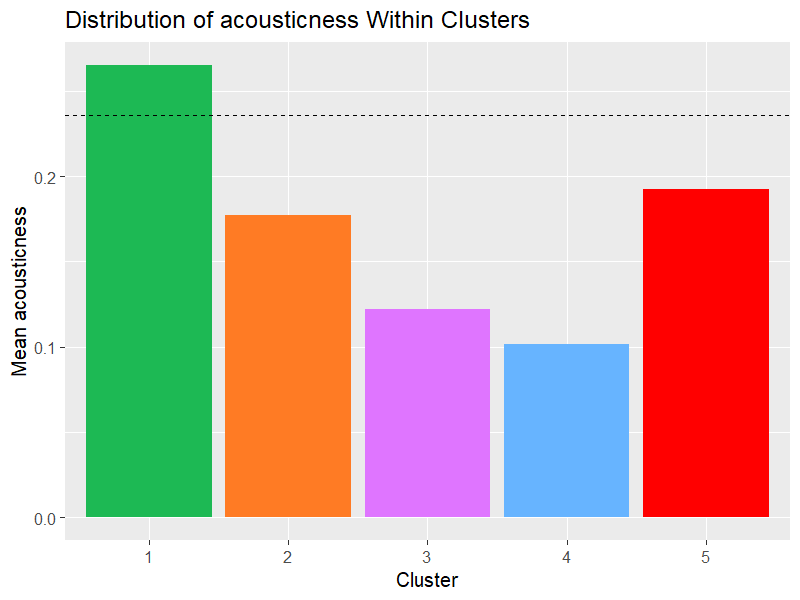
\includegraphics[width=0.95\linewidth]{Images//8_Textual//LSA/profiling_acousticness.png}
        \caption{Acousticness per clúster}
        \label{fig:textual_lsa_profiling_acoust}
    \end{minipage}%
    \begin{minipage}{.4\textwidth}
        \centering
        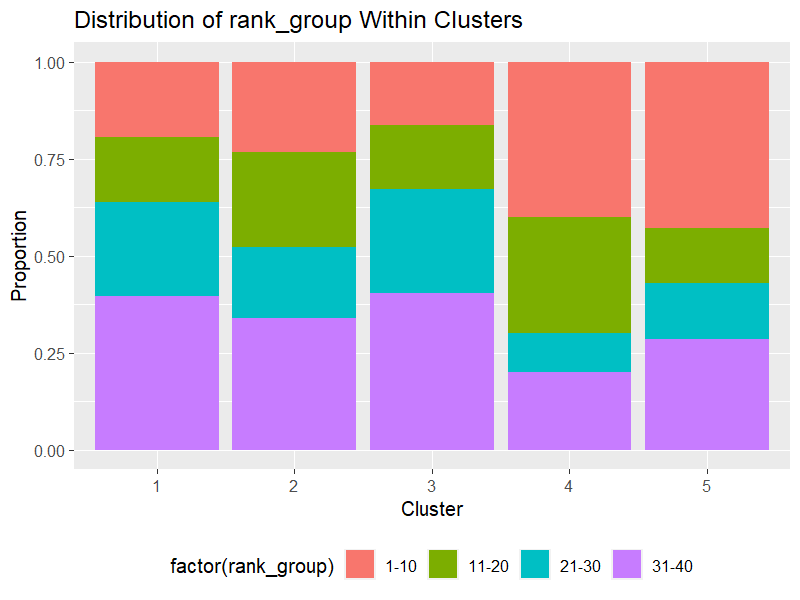
\includegraphics[width=0.95\linewidth]{Images//8_Textual//LSA/profiling_rank_group.png}
        \caption{Rank group per clúster}
        \label{fig:textual_lsa_profiling_rank}
    \end{minipage}%
\end{figure}

\begin{figure}[H]
    \centering
    \begin{minipage}{.4\textwidth}
        \centering
        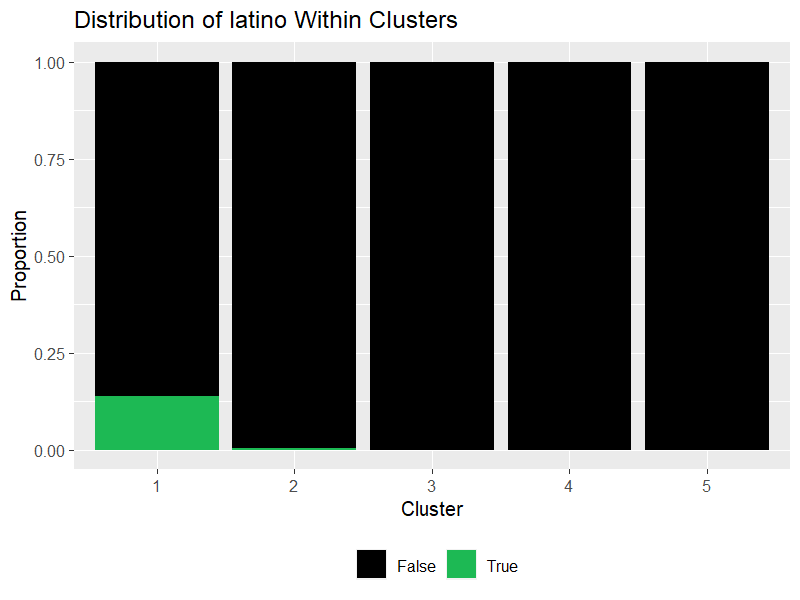
\includegraphics[width=0.95\linewidth]{Images//8_Textual//LSA/profiling_latino.png}
        \caption{Proporció de latino per clúster}
        \label{fig:textual_lsa_profiling_latino}
    \end{minipage}%
    \begin{minipage}{.4\textwidth}
        \centering
        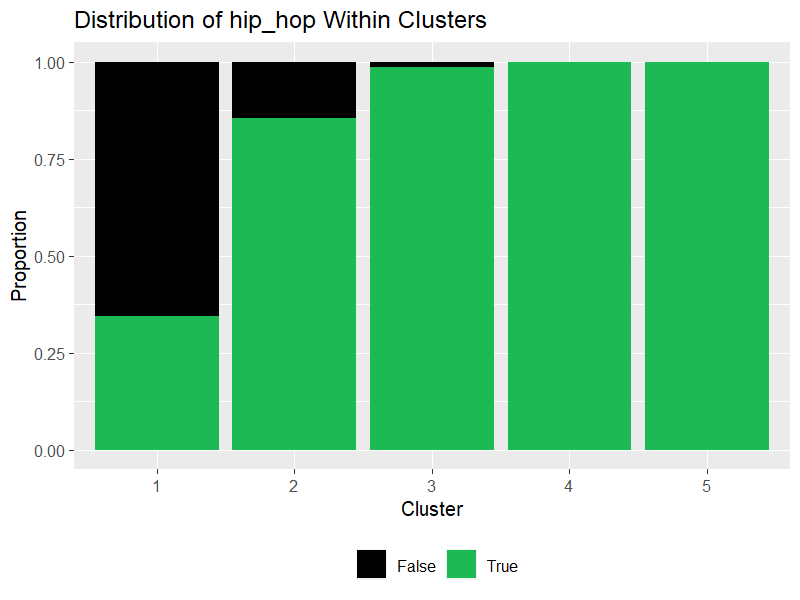
\includegraphics[width=0.95\linewidth]{Images//8_Textual//LSA/profiling_hip_hop.png}
        \caption{Proporció de hip hop per clúster}
        \label{fig:textual_lsa_profiling_hiphop}
    \end{minipage}%
\end{figure}

S'observa com el grup 1 conté les cançons més acústiques, mentre que el 4 les menys \ref{fig:textual_lsa_profiling_acoust}. Com era d'esperar, els grups 3,4 i 5 són totalment de hip hop, i el 2 també bastant \ref{fig:textual_lsa_profiling_hiphop}. A més, les cançons latino s'han agrupat en el primer clúster \ref{fig:textual_lsa_profiling_latino}. Sembla ser que els clústers 4 i 5 contenen les cançons més exitoses de hip hop (\ref{fig:textual_lsa_profiling_rank}), i lo que els diferencia és la positivitat (4 són poc acústiques i positives, el 5 més negatives i menys enèrgiques) \ref{fig:textual_lsa_profiling_val}.

Pel que fa les paraulesm és usades, no hi ha gaire diferència, o sigui que per aquest clústering en concret no ajuden gaire a analitzar els grups \ref{fig:textual_lsa_profiling_words}.

Amb tot el que hem realitzat, s'ha vist com l'LSA és capaç de trobar associacions entre els documents. A més, també s'ha detectat com és molt útil per trobar cançons similars, i com sembla ser que els diferents gèneres musicals contenen cançons que tracten de temes semblants.

\newpage
\subsection{Assignació de Dirichet Latent}

\subsubsection{Preprocessament dels textos}

Abans de començar a dur a terme l'anàlisi, és molt recomanable passar els textos per un petit preprocessament, en el que es treguin les diferents paraules o símbols que no aportin variància a l'hora de realitzar els dos models. En aquest cas, s'ha decidit fer les següents operacions:

\begin{itemize}
    \item Transformar tot el text a minúscules, amb l'objectiu de no considerar dues paraules iguals amb diferents capitalitzacions com a paraules diferents.
    \item Eliminar els nombres del text, ja que per aquest tipus d'anàlisi no afegeix variància (es tracta d'anàlisis no sensibles al context.
    \item Eliminar les \textit{stopwords} en anglès i castellà. A causa de la gran freqüència en la qual aquestes paraules apareixen al text, i la poca informació que poden aportar a un document, hem decidit esborrar aquelles dels dos idiomes més populars a la nostra base de dades, l'anglès i el castellà.
    \item Eliminar els diferents signes de puntuació, pel soroll que afegeixen en dur a terme anàlisis basades en freqüències.
    \item Esborrar dels textos totes aquelles paraules que vam trobar com a paraules no informatives al realitzar un primer anàlisi, amb paraules onomatopeiques, principalment, com \textit{yeah}, \textit{ere} o \textit{ahn}. 
\end{itemize}

Un cop aplicat aquest petit procés, els resultats obtinguts pels models tindran molt més sentit, gràcies a aquest esborrament de paraules que afegeixen més soroll que informació.

\newpage

\subsubsection{Selecció del nombre de tòpics}
Donat que l'algorisme LDA requereix un paràmetre \textit{k} que escolli el nombre de tòpics en els quals es separaran els diferents documents, cal escollir una \textit{k} que maximitzi el sentit dels tòpics trobats. Amb tal d'escollir aquesta \textit{k}, s'han agafat les diferents mesures de 4 mètriques proporcionades per la funció \textit{FindTopicsNumber} del paquet utilitzat pel \textit{LDA}.

A la figura \ref{fig:8_LDA:lda_finetunning}, es poden veure els resultats de les diferents mètriques amb \textit{k}'s del 2 al 20. Com es pot comprovar, trobem pics als valors 6 i 8, indicant que, segons les dues mètriques en les quals sí que es troben variacions, és probable que tinguin una mica més de sentit que la resta de tòpics trobats amb altres valors de \textit{k}. Per un altra banda, les mètriques d'\textit{Arun} i \textit{Griffiths} no aporten molta informació, ja que només tenen una tendència a decréixer i créixer respectivament amb el creixement de la \textit{k}.

\begin{figure}[H]
    \centering
    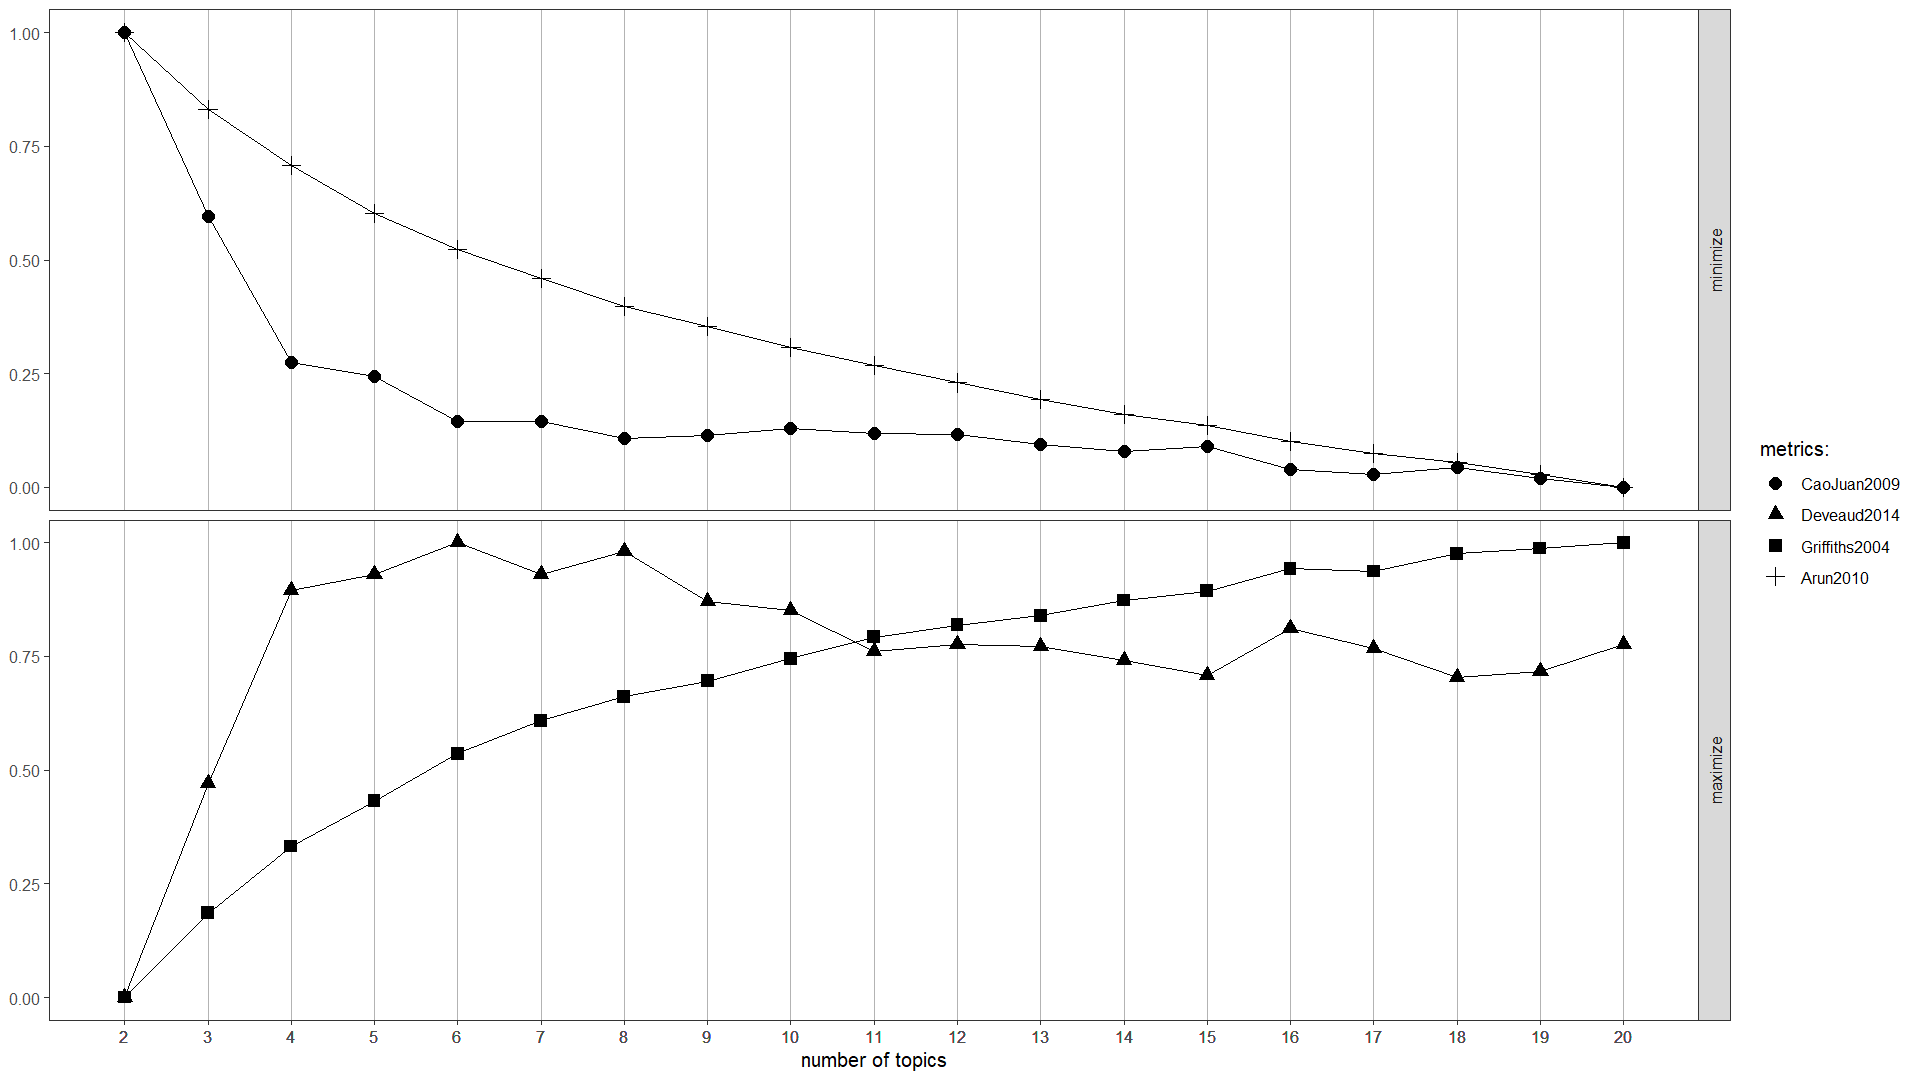
\includegraphics[width=0.7\linewidth]{Images/8_Textual/LDA/lda_finetunning.png}
    \caption{Resultats de les 4 mètriques segons els valors de \textit{k}.}
    \label{fig:8_LDA:lda_finetunning}
\end{figure}

Així doncs, escollim els valors 6 i 8, i comprovem la qualitat dels tòpics escollits. En les figures \ref{fig:LDA:topics6} i \ref{fig:LDA:topics8} trobem els diferents valors de beta pel top 10 paraules amb major beta per cada tòpic (seguint beta el valor que determina la influència que té cada paraula en cadascun dels tòpics). Tal com es pot veure a la figura \ref{fig:LDA:topics6}, fa una clara distinció entre paraules explícites o malsonants al tòpic número 2 i paraules espanyoles al número 3. La resta de tòpics, en canvi, venen a ser bastant més genèrics, amb el tòpic 1 representant un sentiment d'alegria molt genèric, format per paraules com \textit{time}, \textit{dance}, \textit{christmas} o \textit{man}; amb el 4 i el 5 més orientats cap a l'amor amb paraules com \textit{baby}, \textit{feel} o \textit{heart} i el 6 cap a la sensació de nostàlgia o l'abstracció, amb paraules com \textit{mind}, \textit{feel}, \textit{time} o \textit{die}.

Per una altra banda, les paraules principals de les divisions generades amb \textit{k} = 8, són les següents: Els tòpics 1, 2 i 3, segueixen els mateixos patrons que en la divisió anterior, amb el número 1 representant una sensació d'alegria, el 2 insults en anglès i el 3 paraules en castellà. Els tòpics 4, 5 i 6 també s'assemblen als anteriors, representant l'amor el 4 i el 5, i la nostàlgia el 6. Finalment, els tòpics 7 i 8 no ens arriben a donar cap tema nou, ja que el 7 sembla representar el tema de l'amor un altre cop i el 8 insults o ``\textit{slangs}'' en anglès, tot i que en aquest cas no predominen tant els insults, i també trobem paraules que indiquen la voluntat de fer, molt comuns en cançons de \textit{hip hop}.

\begin{figure}[H]
    \centering
    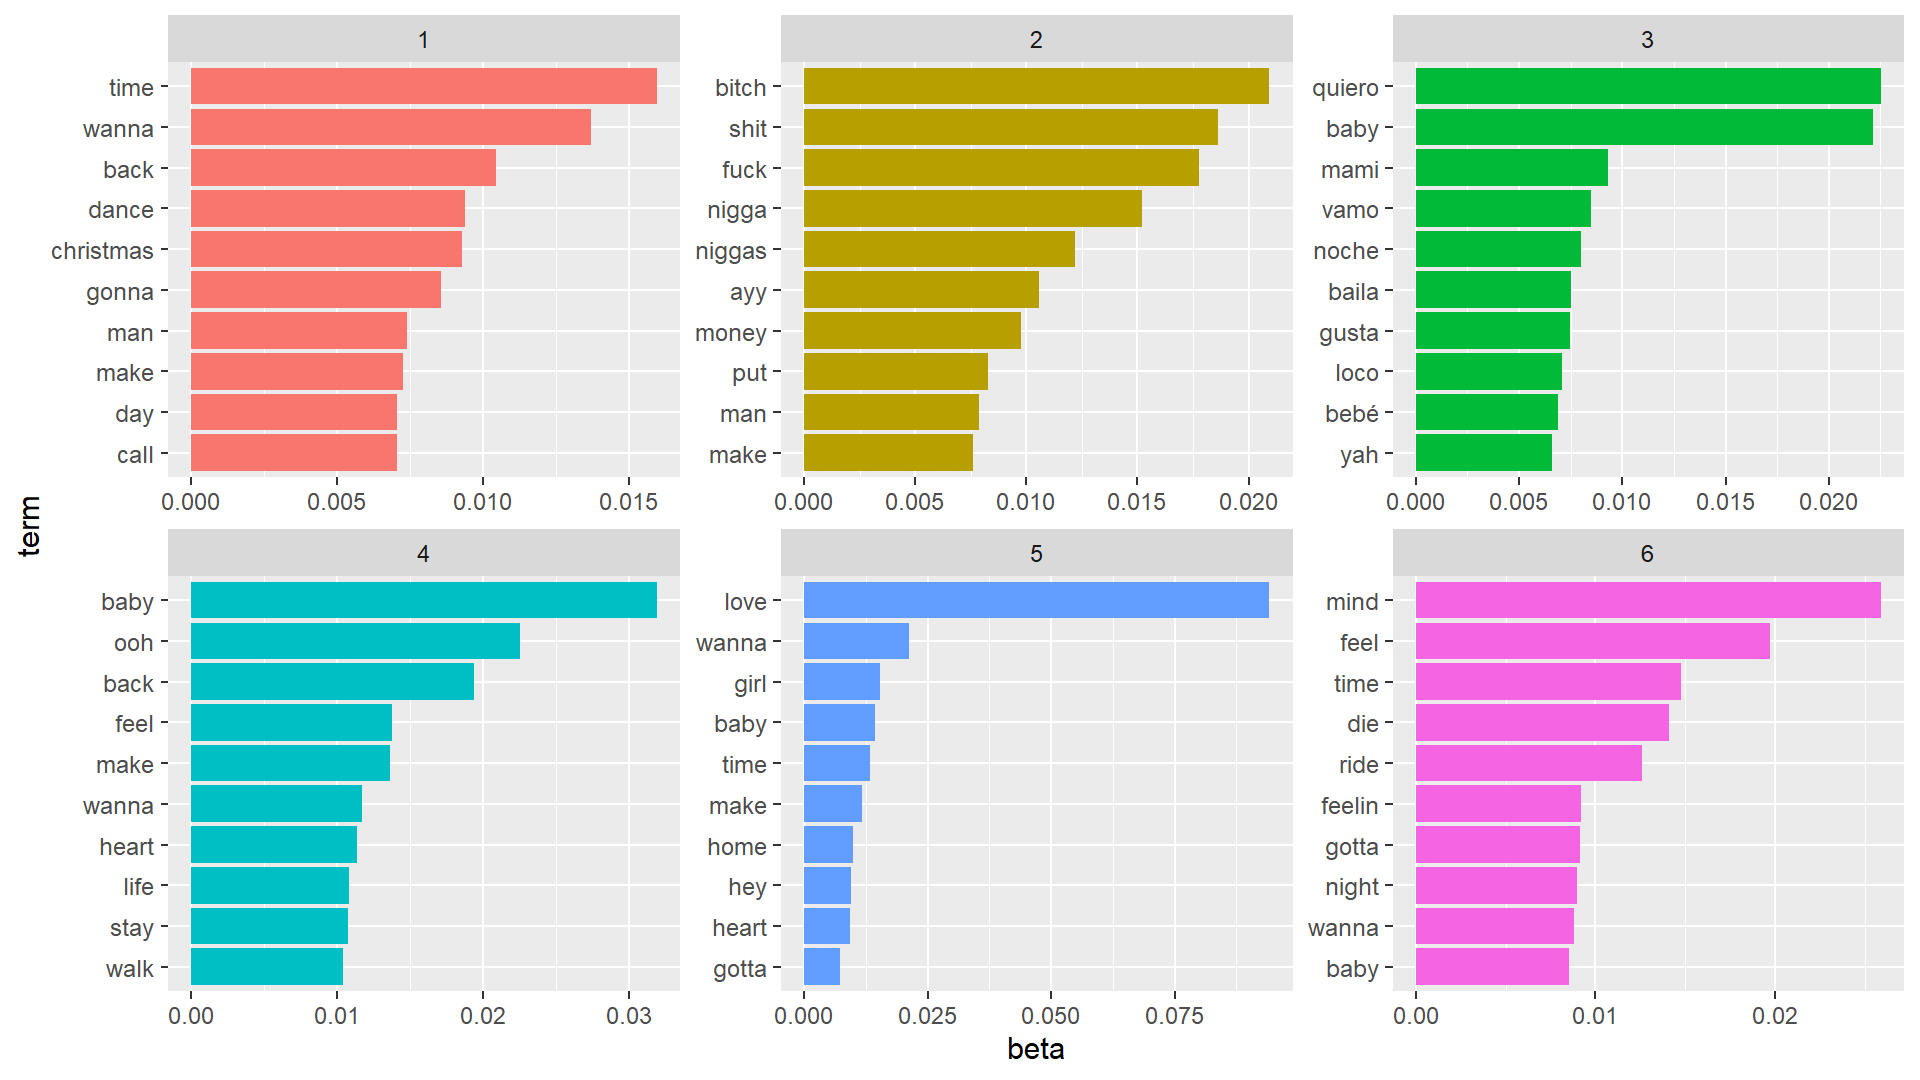
\includegraphics[width=0.8\linewidth]{Images/8_Textual/LDA/lda_topics6.png}
    \caption{Paraules amb més pes en els tòpics creats amb \textit{k} = 6, segons les betes trobades pel model}
    \label{fig:LDA:topics6}
\end{figure}

\begin{figure}[H]
    \centering
    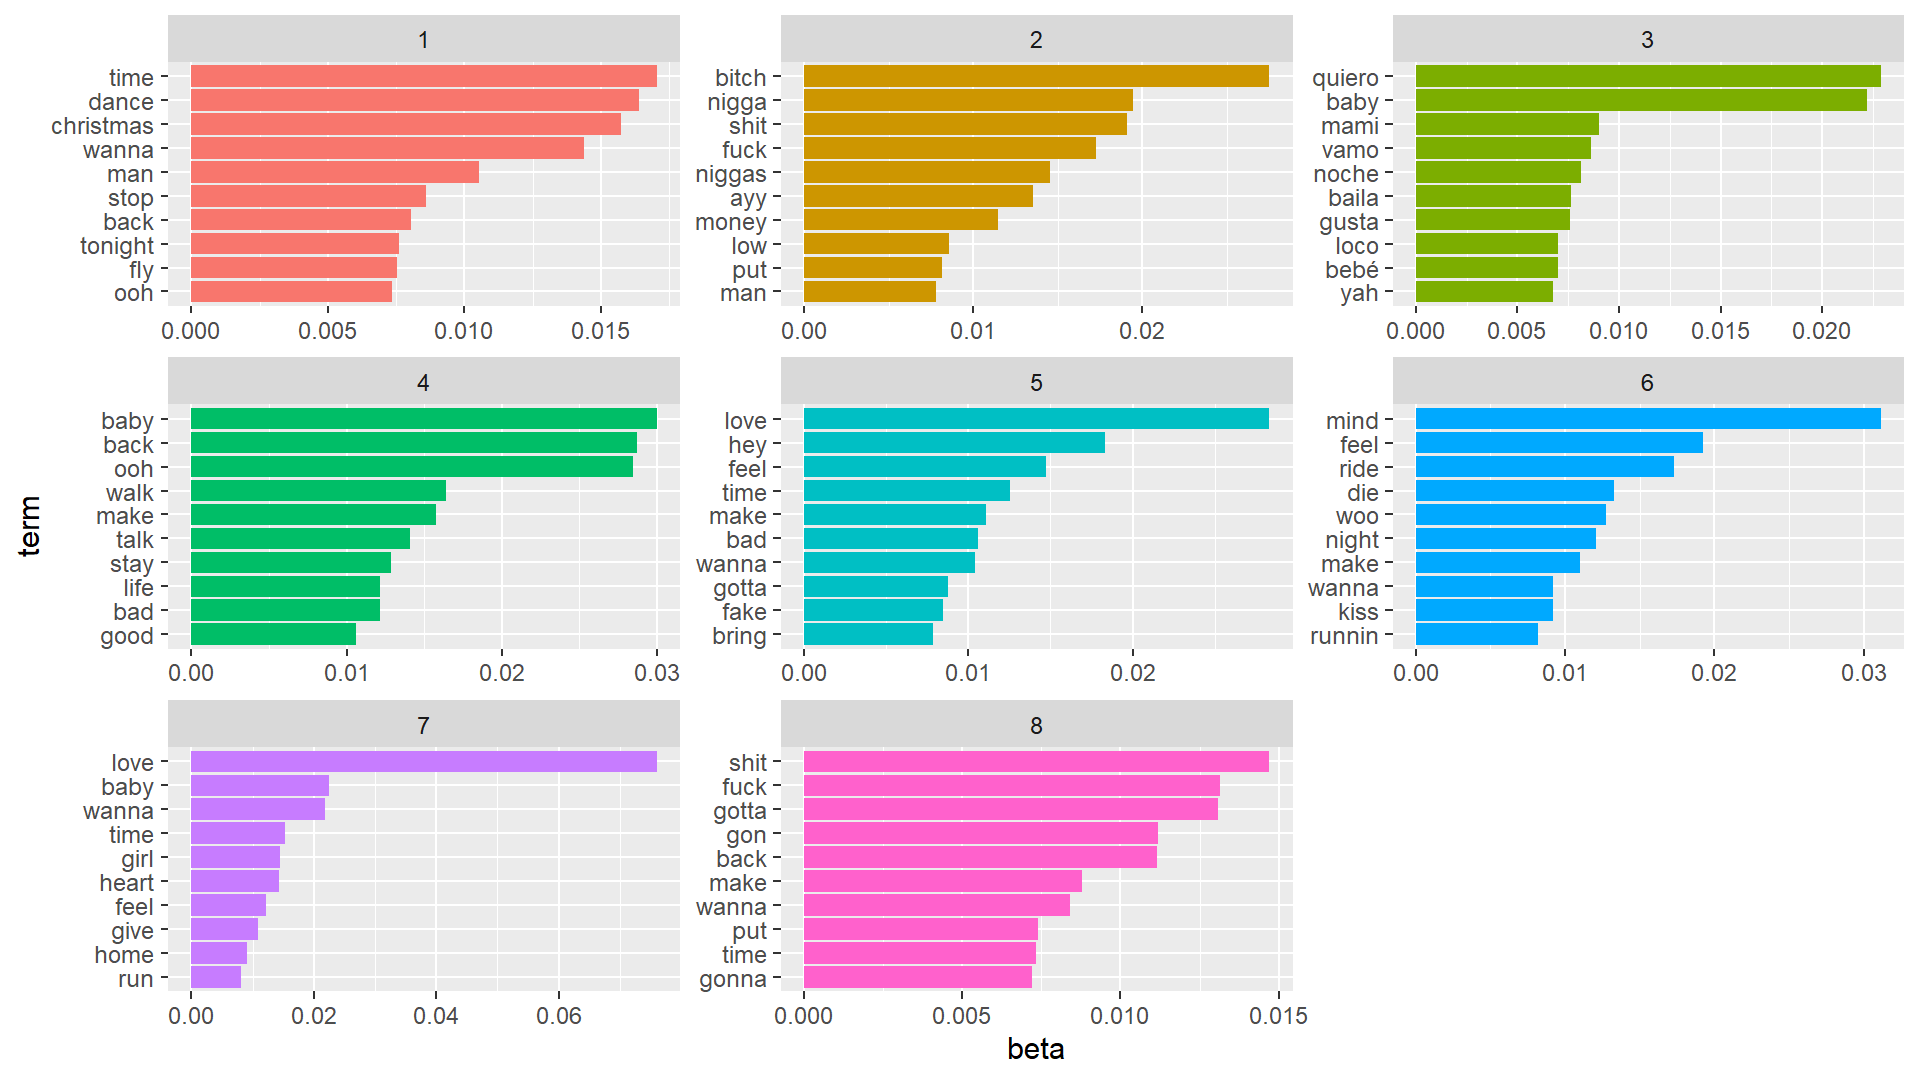
\includegraphics[width=0.8\linewidth]{Images/8_Textual/LDA/lda_topics8.png}
    \caption{Paraules amb més pes en els tòpics creats amb \textit{k} = 8, segons les betes trobades pel model}
    \label{fig:LDA:topics8}
\end{figure}

Donats aquests resultats, i la repetició que trobem en els 2 nous tòpics generats en escollir un model de 8 tòpics en cop de 6, s'ha decidit dur a terme l'anàlisi amb els 6 tòpics en lloc d'amb 8.

\subsubsection{Profiling dels tòpics trobats}

Havent-se escollit i generat ja els tòpics i el model LDA, amb una \textit{k} de valor 6 (veure figura \ref{fig:LDA:topics6}), procedim a fer un profiling dels tòpics obtinguts, amb l'objectiu de trobar diferents patrons o informació de la variable textual (les líriques de les cançons, en aquest cas). Abans de profunditzar, a la secció prèvia, només observant les paraules amb més influència per cadascun dels tòpics, ja hem aconseguit posar-li un nom que resumeixi de forma molt breu el que podrien representar aquestes paraules més freqüents, quedant els següents títols per a cada tòpic:

\begin{itemize}
    \item 1: alegria genèrica
    \item 2: malsonant
    \item 3: castellà
    \item 4: amor 1
    \item 5: amor 2
    \item 6: nostàlgia abstracta
\end{itemize}

Si comparem amb les diferents variables de la nostre base de dades, es troben algunes conclusions que quadren amb els noms assignats als 6 tòpics. Si mirem la comparació amb els gèneres (figura \ref{fig:LDA:genre_profiling}), trobem que els tòpics 2 i 3 estan caracteritzats per una major presència de \textit{hip hop}, el 3 conté pràcticament totes les cançons de \textit{latino}, i \textit{pop} predomina en els tòpics restants (1, 4, 5 i 6). A més, veiem com les cançons de nadal s'agrupen també en el primer tòpic. En el que a la variable \textit{explicit} es refereix, la trobem completament concentrada al tòpic número 2 (veure figura \ref{fig:LDA:genre_profiling}), explicant que aquest tòpic ha separat clarament les cançons de \textit{hip hop} malsonants. A més, els tòpics 4, 5 i 6 semblen contenir més cançons electròniques, tot i que no és tan notable com les relacions prèvies.

\begin{figure}[H]
    \centering
    \includegraphics[width=0.95\linewidth]{Images/8_Textual/LDA/profiling_genres.png}
    \caption{Comparació entre els tòpics trobats i les variables categòriques binaries expressant el gènere i lo malsonant que són les cançons}
    \label{fig:LDA:genre_profiling}
\end{figure}

Per una altra banda, fixant-se en les relacions entre les variables numèriques més característiques de la base de dades i els diferents tòpics, es pot deduir alguna característica dels tòpics trobats. Com es pot veure a la figura \ref{fig:LDA:num_profiling}, els tòpics 2 i 3 tornen a marcar més diferències que els 4 restants. En el cas del tòpic ``\textit{malsonant}'', destaca l'alt nivell de \textit{danceability}, \textit{tempo} i \textit{speechiness}, l'últim segurament sigui conseqüència del gran nombre de cançons de \textit{hip\_hop}, cançons que solen incloure molta més lletra que les de la resta de gèneres. A més, destaquen també els baixos nivells de \textit{artist\_followers} i \textit{acousticness}. Per una altra banda, el tòpic ``\textit{castellà}'' conté alts nivells \textit{danceability}, \textit{energy}, \textit{loudness} i \textit{valence}, junt amb un nivell mitjà més baix de \textit{tempo} que la resta de tòpics. Així i tot, la resta de tòpics (``\textit{alegria}'', ``\textit{amor 1}'', ``\textit{amor 2}'' i ``\textit{nostàlgia}'') no presenten grans variàncies entre ells, en el que a les variables numèriques respecta.

\begin{figure}[H]
    \centering
    \includegraphics[width=0.95\linewidth]{Images/8_Textual/LDA/profiling_nums.png}
    \caption{Comparació mitjançant boxplots múltiples entre els tòpics trobats i les variables numèriques més rellevants de la base de dades}
    \label{fig:LDA:num_profiling}
\end{figure}

Finalment, mirant les 6 variables categòriques que no són ni \textit{explicit} ni els diferents gèneres, s'obtenen els resultats de les figures \ref{fig:LDA:cat2_profiling} i \ref{fig:LDA:bin2_profiling}. Com es pot observar, el nombre d'artistes varia en el tòpic ``\textit{castellà}'', obtenint una major proporció d'artistes en les cançons d'aquest tòpic. També trobem una quantitat de dones menor als tòpics ``\textit{castellà}'' i ``\textit{malsonant}'', mentre que a la resta de tòpics, la proporció es manté de forma semblant. En el que a les variables binàries respecta (fig \ref{fig:LDA:bin2_profiling}), trobem moltes més col·laboracions en ``\textit{malsonant}'' i ``\textit{castellà}'', que en la resta de tòpics. També cal destacar la proporció més gran de cançons on els artistes són un grup al tòpic ``\textit{amor 2}'', tot i que no es tracta d'una diferència abismal.

\begin{figure}[H]
    \centering
    \includegraphics[width=0.95\linewidth]{Images/8_Textual/LDA/profiling_cats_2.png}
    \caption{Profiling de les variables categòriques restants}
    \label{fig:LDA:cat2_profiling}
\end{figure}

\begin{figure}[H]
    \centering
    \includegraphics[width=0.95\linewidth]{Images/8_Textual/LDA/profiling_bins_2.png}
    \caption{Profiling de les variables binàries restants}
    \label{fig:LDA:bin2_profiling}
\end{figure}

Finalment, mirant les 6 variables categòriques que no són ni \textit{explicit} ni els diferents gèneres, s'obtenen els resultats de les figures \ref{fig:LDA:cat2_profiling} i \ref{fig:LDA:bin2_profiling}. Com es pot observar, el nombre d'artistes varia en el tòpic ``\textit{castellà}'', obtenint una major proporció d'artistes en les cançons d'aquest tòpic. També trobem una quantitat de dones menor als tòpics ``\textit{castellà}'' i ``\textit{malsonant}'', mentre que a la resta de tòpics, la proporció es manté de forma semblant. En el que a les variables binàries respecta (fig \ref{fig:LDA:bin2_profiling}), trobem moltes més col·laboracions en ``\textit{malsonant}'' i ``\textit{castellà}'', que en la resta de tòpics. També cal destacar la proporció més gran de cançons on els artistes són un grup al tòpic ``\textit{amor 2}'', tot i que no es tracta d'una diferència abismal.

\begin{figure}[H]
    \centering
    \includegraphics[width=0.95\linewidth]{Images/8_Textual/LDA/profiling_cats_2.png}
    \caption{Profiling de les variables categòriques restants}
    \label{fig:LDA:cat2_profiling}
\end{figure}

\begin{figure}[H]
    \centering
    \includegraphics[width=0.95\linewidth]{Images/8_Textual/LDA/profiling_bins_2.png}
    \caption{Profiling de les variables binàries restants}
    \label{fig:LDA:bin2_profiling}
\end{figure}


\subsubsection{Projecció de les paraules i documents}

A més de dur a terme el profiling anterior dels tòpics, també es representaran tant les paraules com els documents mitjançant una reducció de dimensionalitat de les \textit{betas} i \textit{gammas} respectivament. És a dir, donat un vector generat pel model LDA que representi la importància de una paraula o documents amb tants components com tòpics hagin (6 en aquest cas), es fa una reducció de dimensionalitat amb tal d'observar l'espai generat pel model. Es fa servir un \textit{MDS} (MultiDimensional Scaler), quedant les següents figures \ref{fig:LDA:MDS_paraules_full}, \ref{fig:LDA:MDS_paraules_zoom} i \ref{fig:LDA:MDS_paraules_topic} en el cas de la representació de paraules.

\begin{figure}[H]
    \centering
    \includegraphics[width=0.95\linewidth]{Images/8_Textual/LDA/MDS_paraules_full.png}
    \caption{Representació de les paraules segons les betes trobades pel \textit{LDA}}
    \label{fig:LDA:MDS_paraules_full}
\end{figure}


\begin{figure}[H]
    \centering
    \includegraphics[width=0.95\linewidth]{Images/8_Textual/LDA/MDS_paraules_zoom.png}
    \caption{Representació de les paraules segons les betes fent zoom en el cúmul dret superior, amb l'objectiu de visualitzar millor les paraules}
    \label{fig:LDA:MDS_paraules_zoom}
\end{figure}

Tal com es pot veure a la figura \ref{fig:LDA:MDS_paraules_full}, la veritat és que no sembla que hi hagi moltes relacions entre els significats de les paraules i la seva representació mitjançant el vector de betes. Tot i això, si trobem paraules més malsonants en la part superior dreta, cosa que s'aprecia molt millor observant la figura \ref{fig:LDA:MDS_paraules_zoom}. Si observem la figura \ref{fig:LDA:MDS_paraules_topic}, on trobem les diferents paraules acolorides segons el seu tòpic ``principal'' (el de major beta), trobem que, efectivament, les paraules del tòpic malsonants tendeixen a situar-se dalt a la dreta. A més trobem també com les paraules d'amor 2 es troben en la part inferior, indicant que el segon eix podria representar una relació inversa entre paraules més afectuoses en la part negativa i més explícites o malsonants al costat positiu. Així i tot, no trobem tampoc que aquest tipus de vectorització aporti cap informació ni representació de paraules rellevant.

\begin{figure}[H]
    \centering
    \includegraphics[width=0.95\linewidth]{Images/8_Textual/LDA/MDS_paraules_topic.png}
    \caption{Representació de les paraules segons les betes fent zoom en el cúmul dret superior, amb l'objectiu de visualitzar millor les paraules}
    \label{fig:LDA:MDS_paraules_topic}
\end{figure}

En el que a la projecció de documents respecta, com a primer gràfic trobem la figura \ref{fig:LDA:MDS_paraules_topic}. Aquest ens indica el nom de 10\% de les cançons representades, com que amb més noms la llegibilitat dels noms empitjora bastant. Tot i això, comprovem clarament com les cançons situades a l'esquerra de la gràfica pertanyen al gènere de \textit{hip\_hop}, mentre que les situades a la dreta són cançons més electròniques. Entre aquests extrems trobem cançons de rock i pop, situades lleugerament a la dreta. Evidentment, cal destacar també el cúmul de cançons trobades en el racó inferior dreta, pertanyen aquest tipus de cançons a aquelles cançons amb la lírica en castellà. 

\begin{figure}[H]
    \centering
    \includegraphics[width=0.95\linewidth]{Images/8_Textual/LDA/MDS_docs_10percnt.png}
    \caption{Representació del 10\% de documents segons les gammas trobades pel model amb el seu nom de cançó corresponent}
    \label{fig:LDA:MDS_docs_10percnt}
\end{figure}

Si acolorim els punts en funció d'algunes variables categòriques (veure figura \ref{fig:LDA:MDS_docs_filtered}), trobem relació directa amb lo mencionat al paràgraf previ. Es veu perfectament, com les cançons explícites són principalment aquelles localitzades en la part negativa del primer eix, formant un peculiar triangle. Aquestes cançons, coincideixen també amb el gènere \textit{hip\_hop}, com es pot comprovar a la mateixa figura \ref{fig:LDA:MDS_docs_filtered}. La relació inversa es presenta al mirar el gènere \textit{pop}, on trobem la majoria de cançons d'aquest gènere a la dreta del primer eix. També es pot veure com les cançons del gènere \textit{electro} es troben també cap a la dreta del gràfic. Cal remarcar també la concentració del gènere \textit{latino} sota a la dreta, tal com s'ha explicat al paràgraf previ. 

\begin{figure}[H]
    \centering
    \includegraphics[width=0.95\linewidth]{Images/8_Textual/LDA/MDS_docs_filtered.png}
    \caption{Representació dels documents segons les gammas trobades pel model i acolorits segons diferents modalitats de variables categòriques}
    \label{fig:LDA:MDS_docs_filtered}
\end{figure}

Finalment, al acolorir aquesta representació de la reducció de dimensionalitat segons el tòpic amb el que més relació té cadascun dels documents segons el model, trobem una clara representació de com s'han classificat els diferents documents (figura \ref{fig:LDA:MDS_docs_by_topic}). Com es pot comprovar, ``\textit{alegria}'' es troba just entre ``\textit{amor 1}'' i ``\textit{nostàlgia}'', quasi de forma paral·lela, i ``\textit{amor 2}'' i ``\textit{alegria}'' coincideixen en gran part de la representació. Això explica gran part de les poques diferències trobades entre aquests 4 grups. A més, es pot veure com malsonant i castellà es diferencien d'aquests 4 grups.

\begin{figure}[H]
    \centering
    \includegraphics[width=0.95\linewidth]{Images/8_Textual/LDA/MDS_docs_by_topic.png}
    \caption{Representació dels documents segons les gammas trobades pel model i acolorits segons el seu tòpic principal}
    \label{fig:LDA:MDS_docs_by_topic}
\end{figure}


\subsubsection{Anàlisi temporal dels tòpics trobats}

Finalment, compararem els tòpics amb les variables temporals mitjançant \textit{time series}'es amb el fin d'avaluar encara més els tòpics trobats pel model \textit{LDA}. Donades les nostres dos tipus de variables temporals (unes per indicar la sortida de la cançó i altres per representar la setmana en la que cada cançó s'ha trobat a la base de dades), obtindrem dues gràfiques diferents.

Per una banda, observant la figura \ref{fig:LDA:topics_temporal_sortida} trobem una tendència creixent a les cançons del tòpic ''\textit{castellà}'', en els últims anys, tot i que sembla que a 2021 s'hagi perdut tota aquesta tendència. ''\textit{Alegria}'' en canvi, sembla no tenir cap tendència predictible, amb un clar pic en primavera del 2021 i un vall a l'hivern de 2019. El tòpic ''\textit{malsonant}'' té uns pics bastant peculiars l'any 2018 i 2020, on trobem com els artistes d'aquest tòpic tendeixen a publicar cançons duran la primavera i estiu (any-2 i any-3). En el que a ''\textit{amor 1}'' respecta, hi ha un petit pic l'any 2017, però la resta és bastant estable, amb una petita decadència els últims dos anys. Finalment, ''\textit{amor 2}'' no té cap característica molt destacable, i de nostàlgia es pot marcar l'alt nombre de pics i valls que té. En general, podem dir que aquestes gràfiques no aporten molta informació rellevant, a part de la creixent tendència del tòpic ''\textit{castellà}''.

\begin{figure}[H]
    \centering
    \includegraphics[width=0.98\linewidth]{Images/8_Textual/LDA/topics_temporal_sortida.png}
    \caption{Seguiment temporal de les dates de sortida de les cançons classificades segons el seu tòpic més influent}
    \label{fig:LDA:topics_temporal_sortida}
\end{figure}

Per una altra banda, si observem la figura \ref{fig:LDA:topics_temporal_setmana}, veurem les tendències d'escolta de la gent, ja que mostra les freqüències de cançons segons les dates en les quals s'han trobat al top 40 del rànquing. En el que a ''\textit{alegria}'' respecta, trobem pics als hiverns, conseqüència segurament de les cançons de Nadal trobant-se dins d'aquest tòpic. Així i tot, és estrany que l'any 2019 no hi hagués un pic. En ''\textit{malsonant}'', hi ha un gran pic en 2018, i es veu que és un tòpic en decadència en el que al top 40 respecta. En ''\textit{castellà}'' trobem dos pics, en 2019 i a la tardor de 2020. També podríem intuir una petita tendència a créixer en aquest tipus de cançons. En el que a ''\textit{amor 1}'' es refereix, hi ha un pic a la tardor de 2017 i un petit vall a l'estiu de 2018, tot i que és un tòpic bastant estable, amb moltes cançons al top 40. Del tòpic ''\textit{amor 2}'' no podem dir el mateix, ja que tenim una clara tendència a decréixer amb petits pics i valls. Finalment, nostàlgia és el tòpic amb menys cançons al top 40 durant aquest període de temps, amb un pic extens en 2018 i una clara caiguda a partir de 2020.

\begin{figure}[H]
    \centering
    \includegraphics[width=0.98\linewidth]{Images/8_Textual/LDA/topics_temporal_setmana.png}
    \caption{Seguiment temporal de les dates en les que les cançons es trobaven al top 40, classificades segons el seu tòpic més influent}
    \label{fig:LDA:topics_temporal_setmana}
\end{figure}








\subsection{Creació de playlists personalitzades}

Tenint en compte que el nostre \textit{dataset} tracta sobre música, on les lletres tenen un paper principal, i veient els bons resultats observats en la secció de \textit{LSA} \ref{LSA}, es va decidir intentar crear una aplicació real fent ús d'aquestes eines centrades en texts. 

Una idea inicial que es va pensar va ser el procés de creació de \textit{playlists} personalitzades utilitzant l'anàlisi semàntica latent degut a la capacitat d'aquest sistema per obtenir similituds entre documents.

Aquest petit projecte consisteix en interpretar les preferències de l'usuari a partir d'una frase i un conjunt de filtres, per després trobar cançons similars en un corpus de lletres de cançons que en aquest cas és el top 40 cançons setmanals. A continuació, es descriuen les etapes principals del procés.

\subsubsection{Neteja del corpus}

Per tal de preparar el corpus per l'anàlisi, es duen a terme diverses transformacions:

\begin{itemize}
    \item Conversió de tot el text a minúscules.
    \item Eliminació de números i paraules sense significat (stopwords) en anglès.
    \item Eliminació de signes de puntuació i espais en blanc innecessaris.
    \item Eliminació de paraules específiques com "tis".
\end{itemize}

\subsubsection{Extensió de la frase}

Degut a que la majoria de cançons tenen entre 1500 i 3000 caràcters i tenint en compte que l'usuari molt probablement vulgui cançons similars a una frase senzilla la qual, per exemple, pot tenir al voltant de 50 caràcters, l'LSA donaria tots els documents pràcticament com igual de similars degut a la gran diferència de llargada.

Per evitar aquest error vam decidir que donada una frase aquesta tingui una longitud mínima fixada en 1500 caràcters, estenent la mateixa frase fins a arribar a aquesta longitud requerida.

\subsubsection{Interpretació de la sol·licitud de l'usuari}

Per tal d'interpretar les sol·licituds extres anomenats \textit{requests} de l'usuari es van definir diversos filtres per interpretar aquestes preferències; aquestes inclouen:

\begin{itemize}
    \item \textbf{Gènere}: Identificació del gènere musical a partir de paraules clau.
    \item \textbf{Ballabilitat}: Classificació de la cançó com a molt bailable o bailable segons les paraules clau.
    \item \textbf{Acústica}: Identificació de cançons acústiques a partir de paraules clau.
    \item \textbf{València}: Identificació de cançons tristes a partir de paraules clau.
    \item \textbf{Contingut explícit}: Filtratge segons si la cançó conté o no contingut explícit.
    \item \textbf{País}: Identificació de la nacionalitat de l'artista.
    \item \textbf{Artista}: Identificació específica d'un artista mencionat.
    \item \textbf{Gènere de l'artista}: Identificació del gènere de l'artista a partir de paraules clau.
    \item \textbf{Idioma}: Identificació de l'idioma de la lletra de la cançó.
    \item \textbf{2024}: En el cas que s'inclogui aquest any, per tal de generar les \textit{playlists} també es tindrà en compte una altra base de dades la qual conta amb més cançons de l'actualitat.
\end{itemize}

\subsubsection{Aplicació de l'LSA i creació de \textit{playlists}}

Un cop netejat el corpus i interpretades les preferències de l'usuari, s'aplica l'anàlisi semàntica latent (LSA) de la següent manera:

\begin{enumerate}
    \item Es crea una matriu terme-document a partir del corpus netejat i la frase d'entrada.
    \item Es calcula la semblança cosinus entre la nova frase i les cançons del corpus.
    \item Es crea un \textit{data frame} amb les semblances i els detalls de les cançons, incloent-hi tots els requisits que l'usuari hagi demanat.
    \item S'apliquen els filtres identificats en la sol·licitud de l'usuari per refinar els resultats.
    \item Les cançons es classifiquen per ordre de semblança, obtenint així les \textit{playlists} de mida \textit{n}, generalment 30, personalitzades.
\end{enumerate}

Finalment per validar aquest projecte s'han utilitzat diferents frases i sol·licituds d'exemple per generar \textit{playlists} personalitzades. Per exemple, per la frase \textit{"Me gustas mucho pero la relación no puede seguir"} i la sol·licitud \textit{"Quiero una canción del género latino que sea muy bailable de Bad Bunny"}, s'ha generat una \textit{playlist} amb les cançons més semblants, considerant els filtres específics de l'usuari obtenint uns resultats molt bons on el sentit semàntic de la frase d'entrada es veia reflexada en les cançons i on els requisits extres també havien servit de filtre.

\subsubsection{Integració amb Spotify}

Per facilitar l'ús de les \textit{playlists} generades, s'ha integrat el sistema amb l'API de Spotify per permetre als usuaris guardar directament les \textit{playlists} a la seva compte de Spotify. El procés es descriu a continuació:

\begin{enumerate}
    \item S'autentica l'usuari amb l'API de Spotify utilitzant les credencials del client.
    \item Es crea una nova \textit{playlist} al compte de l'usuari amb el nom especificat i una descripció.
    \item S'afegeixen les cançons a la nova \textit{playlist} utilitzant els identificadors de les cançons generades.
    \item Es notifica a l'usuari que la \textit{playlist} s'ha creat correctament.
\end{enumerate}

Aquest enfocament proporciona una manera robusta i eficaç de crear \textit{playlists} personalitzades basades en les preferències específiques de l'usuari i l'anàlisi de les lletres de les cançons mitjançant tècniques d'intel·ligència artificial. 

Cal mencionar que \textit{Spotify} no disposa d'un creador de llistes de reproduccions públic i gratuït on tan sols els usuaris \textit{premium} d'alguns països tenen accés a un generador en estat de prova així que aquest producte pot resultar molt útil tant com per a l'empresa com per a tots els usuaris.

\subsection{Predicció del gènere musical d'un text}

Aquest apartat descriu un mètode per predir el gènere musical d'un text basat en l'anàlisi semàntica latent (LSA) i l'ús de k-Nearest Neighbors (k-NN). A continuació es detallen les etapes principals del procés i els resultats de l'avaluació del model.

\subsubsection{Preparació de l'espai LSA}

Per preparar l'espai LSA, es segueixen els passos següents:

\begin{enumerate}
    \item Es crea un corpus a partir de les lletres de les cançons.
    \item Es neteja el corpus utilitzant diverses transformacions, com la conversió a minúscules, l'eliminació de números, paraules sense significat (stopwords) i signes de puntuació.
    \item Es crea una matriu terme-document a partir del corpus netejat.
    \item Es seleccionen els termes amb una freqüència mínima del 3\% respecte al nombre total de cançons. Aquest percentatge és tan baix per tal de fer que predigui millor els gèneres que són minoria.
    \item Es realitza l'anàlisi semàntica latent (LSA) per obtenir l'espai LSA.
\end{enumerate}

\subsubsection{Predicció del gènere utilitzant k-NN i LSA}

El procés de predicció del gènere d'una nova lletra de cançó es realitza mitjançant els passos següents:

\begin{enumerate}
    \item Es preprocessa la nova lletra de la cançó per assegurar que tingui la longitud mínima requerida.
    \item Es combina la nova lletra amb les lletres del corpus existent.
    \item Es neteja el corpus combinat i es crea una nova matriu terme-document.
    \item Es realitza l'LSA per a la nova matriu terme-document.
    \item Es calcula la semblança cosinus entre la nova lletra i les cançons del corpus.
    \item Es seleccionen les k cançons més similars i es compten els gèneres més comuns entre aquestes.
    \item En cas que una cançó pertanyi a més d'un gènere, es fa un ajustament per donar més pes als gèneres \textit{latino} i \textit{christmas} degut a la seva menor representació en el corpus.
    \item Es prediu el gènere basant-se en el gènere més comú entre les k cançons més similars.
\end{enumerate}

Cal mencionar que encara que una cançó pugui pertànyer a més d'un gènere, només es predirà un de sol. En el cas de les cançons \textit{latino} o \textit{christmas}, es dona més pes a aquests gèneres per evitar que es classifiquin incorrectament com \textit{pop} degut a la seva menor representació.

\subsubsection{Avaluació del model}

Per tal d'avaluar l'eficàcia del mètode, es va seleccionar aleatòriament un conjunt de 100 cançons i es va calcular la precisió del model. Per calcular aquesta precisió simplement es va contar com a correcta en el cas que la cançó realment tingués el gènere predit, encara que la propia cançó pugui tenir-ne d'altres. El resultat va ser una precisió del 93\% (93 encerts sobre 100) indicant així que el model té una capacitat molt acceptable i pot ser utilitzat per aquesta tasca de predicció del gènere musical.

\subsubsection{Exemples de predicció de gènere}

A continuació es presenten alguns exemples de predicció de gènere utilitzant el model desenvolupat:

\begin{itemize}
    \item \textbf{Cançó Pop:}
    \begin{quote}
    \textit{"On a starry night, we danced all through the light. Holding hands, feeling right, under the moon so bright. We laughed and we sang, hearts intertwined, In this moment so divine, forever you and I."}
    \end{quote}
    Predicció: \textit{Pop}

    \item \textbf{Cançó Latino:}
    \begin{quote}
    \textit{"Bajo la luna llena, bailamos sin parar, Ritmo en nuestras venas, el mundo a celebrar. Tus ojos me encantan, tu risa es un mar, Juntos hasta el amanecer, no hay nada igual."}
    \end{quote}
    Predicció: \textit{Latino}

    \item \textbf{Cançó Hip Hop:}
    \begin{quote}
    \textit{"In the fucking streets, lights flashing, grinding every night, Fuck the haters, I'm smashing, gotta keep it tight."}
    \end{quote}
    Predicció: \textit{Hip Hop}

    \item \textbf{Cançó de Nadal:}
    \begin{quote}
    \textit{"Snowflakes falling, carols in the air, Family's calling, love everywhere. Lights on the tree, gifts by the fire, Joy, hearts full of desire."}
    \end{quote}
    Predicció: \textit{Christmas}
\end{itemize}

Aquest mètode proporciona una manera eficaç de predir el gènere musical d'una lletra de cançó utilitzant tècniques d'anàlisi semàntica latent i \textit{k-Nearest Neighbors}, amb una alta precisió demostrada en l'avaluació del model. El model pot resultat molt útil a l'empresa de \textit{Spotify} degut a que encara que un cantant no publiqui explícitament quin gènere o categoria té una cançó, poder-la etiquetar sense necessitat d'escoltar-la.


\subsection{Desambiguació de gèneres}

Un dels reptes que es van haver d'afrontar amb el dataset original, en el passat, va ser el d'agrupar els gèneres de música. La base de dades original contenia diversos gèneres per artista, i alguns d'aquests eren molt específics i no ens interessaven. Aquest problema va ser resolt de forma manual, assignant el gènere que es va creure més adient.

Aprofitant que s'ha treballat amb anàlisi textual, s'ha realitzat aquesta agrupació per gèneres d'una forma més automàtica.

\subsubsection{Obtenció de les dades}

El primer pas era obtenir dades sobre els gèneres musicals, per tal de classificar-los. S'ha utilitzat la llibreria rvest per tal d'obtenir aquesta informació de la Wikipedia. Aquestes dades representen un corpus d'informació addicional, que ens permetran obtenir certes relacions entre els conceptes de cada subgènere de música, ja que utilitzaran paraules similars. El procés és el següent.

Carregant la base de dades original, obtenim tots els subgèneres. Aquests noms, llavors, son buscats a la pàgina Wikipedia \textit{List of music genres and styles} (en alguns casos s'han hagut de realitzar excepcions, com en hip hop, pop, dance pop, trap...) i es guarden les seves URL.

A continuació la feina és senzilla: simplement iterar per les URL i guardar els texts (continguts en etiquetes p només, així evitem llistes o altra informació no desitjada). En els casos en els que aquest procés falla, es poden entrar manualment els textos.

\subsubsection{Anàlisi de topics}
Aquests textos s'han utilitzat en una Assignació Latent de Dirichlet (LDA) amb k = 9. Podem observar els termes més importants de cada topic.

\begin{figure}
    \centering
    \includegraphics[width=0.8\linewidth]{Images//8_Textual//Genres/genres_lda_topic_terms.png}
    \caption{Termes més importants de cada un dels topics trobats en els textos dels gèneres}
    \label{fig:textual_genres_lda_topics}
\end{figure}

Observem com sembla haver-hi bastanta diferència entre els topics, i les paraules que aporten més a cada un són interessants. Podem descriure'ls a continuació, assignant un nom a cada un d'ells:

\begin{itemize}
    \item \textbf{Electro-disco-house}: Paraules com electronic, game, house ens indiquen que aquest topic estara freqüentat per músiques de l'estil de l'EDM
    \item \textbf{Reggae i alternatiu}: La paraula reggae ens dona bastantes pistes. Hi hafegim alternatiu ja que hi ha rock que també és important (tot i que no sembla ser el principal gènere, ja que jamaican, dancehall i lofi són més aviat de reggae)
    \item \textbf{Músiques regionals}: Mariachis, gqom, rumba... semblen indicar gèneres diversos que comparteixen el fet de ser locals
    \item \textbf{Hip hop}: Aquest topic clarament és hip hop: trobem hip, hop (ja que les separa), rap, rappers, trap...
    \item \textbf{Soul, r\& b}: Les paraules soul i blues semblen indicar que aquest topic es decanta cap a una espècie de barreja entre jazz i blues, antecessora al rock (també mencionat): el Rhythm and Blues.
    \item \textbf{Rock metal}: Les paraules ho deixen bastant clar: la principal és metal, i trobem també rock, bands (és un tipus de música on no solen haver-hi solistes), punk...
    \item \textbf{Funk}: Aquesta és la paraula principal, però trobem també jazz (d'on prové el funk) i altres mencions a estils més moderns com el house o l'electro (encara que aquests ja els hem agrupat al primer topic)
    \item \textbf{Pop}: Menciona aquesta paraula, així com la música en general, el rock o l'indie. El considerem pop bàsicament perquè és el que li escau més.
    \item \textbf{Country i folk}: Country, folk són pràcticament les úniques paraules que identifiquen aquest topic comparant-lo amb la resta.
\end{itemize}

En definitiva, sembla ser que els topics agrupen els subgèneres en diversos grups principals, que a més trobem interessants. Si visualitzem els resultats, veiem la figura \ref{fig:textual_genres_tsne_topic}.

\begin{figure}[H]
    \centering
    \includegraphics[width=0.7\linewidth]{Images//8_Textual//Genres/genres_tsne_topic_results.png}
    \caption{Visualització dels subgèneres i els topics. De mida més gran, hi ha \textit{hip hop}, \textit{pop} i \textit{afro pop}}
    \label{fig:textual_genres_tsne_topic}
\end{figure}

Al visualitzar-ho utilitzant t-SNE (no lineal), queden els subgèneres agrupats com en clústers, fet que ens permet visualitzar-los més intuitivament (encara que la interpretabilitat de les dimensions és pràcticament nul·la, només ens interessava veure com s'agrupaven les dades). Observem els grups que hem comentat abans, amb alguns outliers que, si bé estan molt a prop del grup d'un topic, pertaneyn a un altre: És el cas de \textit{french house} (alhora amb el house i amb el grup de funk), per exemple, o hard rock (amb el grup de metal, però molt a prop d'altres rocks com el blues rock o el folk punk). De fet, són aquests punts els més interessants, ja que ens permeten visualitzar com en el món de la música, realment els generes se sol·lapen i es barrejen, i no estan totalment aïllats. Per exemple, dins el grup del house, trobem el \textit{hip house} que està més a prop del hip hop. Dins de \textit{pop}, el \textit{pop rap} està tirant cap a \textit{hip hop}, i \textit{smooth jazz} evidentment cap al jazz.

També podem realitzar un KNN, amb les dades, per veure si dona resultats diferents.

\begin{figure}
    \centering
    \includegraphics[width=0.7\linewidth]{Images//8_Textual//Genres/textual_genres_clustering_results.png}
    \caption{Resultats del KNN amb 8 clústers}
    \label{fig:textual_genres_knn}
\end{figure}

Com que la K era 8, ha desaparegut un grup, concretament el de R\&B, que ha passat a formar part de \textit{hip hop}. Excepte alguns casos puntuals, la majoria de subgèneres no han canviat, i s'han mantingut grups molt similars als anteriors. Per tant, s'han considerat els topics trobats com a bons.

\subsubsection{Resultats}
Un cop obtinguts els topics, s'ha realitzat el procés invers: tornar a la nostra base de dades. Com que alguns dels subgèneres no apareixien a la wikipedia (i per tant no estan a la llista) i per facilitar que les cançons tinguin més gèneres, s'ha optat per, a més d'observar el topic, mirar els noms dels subgèneres contenen alguna paraula clau: \textit{pop}, \textit{rap}...

Amb el procés a la inversa, queden tan sols 20 cançons que no pertanyen a cap gènere (algunes no tenien gènere inicial, altres era per exemple \textit{broadway}).

Podem veure cada topic, quins gèneres inicials tenia i amb quanta freqüencia.

\begin{figure}[H]
    \centering
    \begin{minipage}{.4\textwidth}
        \centering
        \includegraphics[width=0.95\linewidth]{Images//8_Textual//Genres/Electro house_subgenres_freq.png}
    \caption{Recompte de subgèneres per Electro}
    \label{fig:textual_genres_subelectro}
    \end{minipage}%
    \begin{minipage}{.4\textwidth}
        \centering
        \includegraphics[width=0.95\linewidth]{Images//8_Textual//Genres/Reggae Alt_subgenres_freq.png}
    \caption{Recompte de subgèneres per Reggae}
    \label{fig:textual_genres_subreggae}
    \end{minipage}%
\end{figure}


\begin{figure}[H]
    \centering
    \begin{minipage}{.4\textwidth}
        \centering
        \includegraphics[width=0.95\linewidth]{Images//8_Textual//Genres/Regional_subgenres_freq.png}
    \caption{Recompte de subgèneres per Regional}
    \label{fig:textual_genres_subregional}
    \end{minipage}%
    \begin{minipage}{.4\textwidth}
        \centering
        \includegraphics[width=0.95\linewidth]{Images//8_Textual//Genres/Hip hop_subgenres_freq.png}
    \caption{Recompte de subgèneres per Hip hop}
    \label{fig:textual_genres_subhiphop}
    \end{minipage}%
\end{figure}

\begin{figure}[H]
    \centering
    \begin{minipage}{.4\textwidth}
        \centering
        \includegraphics[width=0.95\linewidth]{Images//8_Textual//Genres/R&B_subgenres_freq.png}
    \caption{Recompte de subgèneres per R\&B}
    \label{fig:textual_genres_subrnb}
    \end{minipage}%
    \begin{minipage}{.4\textwidth}
        \centering
        \includegraphics[width=0.95\linewidth]{Images//8_Textual//Genres/Rock_subgenres_freq.png}
    \caption{Recompte de subgèneres per Rock}
    \label{fig:textual_genres_subrock}
    \end{minipage}%
\end{figure}


\begin{figure}[H]
    \centering
    \begin{minipage}{.4\textwidth}
        \centering
        \includegraphics[width=0.95\linewidth]{Images//8_Textual//Genres/Latin & Funk_subgenres_freq.png}
    \caption{Recompte de subgèneres per Latin/Funk}
    \label{fig:textual_genres_sublatlin}
    \end{minipage}%
    \begin{minipage}{.4\textwidth}
        \centering
        \includegraphics[width=0.95\linewidth]{Images//8_Textual//Genres/Pop_subgenres_freq.png}
    \caption{Recompte de subgèneres per Pop}
    \label{fig:textual_genres_subpop}
    \end{minipage}%
\end{figure}

\begin{figure}[H]
    \centering
    \includegraphics[width=0.5\linewidth]{Images//8_Textual//Genres/Folk_subgenres_freq.png}
    \caption{Recompte de subgèneres per Folk}
    \label{fig:textual_genres_subfolk}
\end{figure}

Analitzant els resultats amb la base de dades, podem obtenir les freqüències en les que apareixen cada un d'aquests topics o gèneres a la base de dades.
\begin{figure}[H]
    \centering
    \includegraphics[width=0.7\linewidth]{Images//8_Textual//Genres/genres_frequencies.png}
    \caption{Freqüències dels gèneres}
    \label{fig:textual_genre_freq}
\end{figure}

Aquestes freqüències s'assemblen molt a les que ja teniem. La gran majoria de cançons són de pop (712, abans en teniem 682), sent el segon gènere principal el hip hop (441, abans 511). A continuació, hi ha el de latino, amb 193 (abans era el quart amb 102) i l'electro amb 126 (abans 332). La resta de gèneres realment no son gaire comparables amb els que teniem abans: rock tan sols apareixia 25 cops, christmas 22 i cinema 5. Actualment, tenim RnB amb 56, reggae amb 50, i llavors sí que passem a 23 de rock, 10 de folk i tan sols 4 de regional.

Sembla ser que, tot i que alguns d'aquests gèneres tenen molts subgèneres, no són prou populars com per aparèixer suficients vegades en el top 40. De fet, pràcticament totes les aparicions estan relacionades amb el pop (i té sentit, ja que al cap i a la fi és la música més popular).


\subsection{Geo-textual modeling}

Amb els mètodes textuals, s'ha pogut obtenir una variable numèrica que representa la relació d'una cançó en concret amb un determinat tòpic. S'ha observat que aquests tòpics tenen certa relació amb els gèneres musicals, que al seu torn estaven relacionats amb algunes regions determinades del món. En aquest apartat, s'acabarà d'establir aquesta relació i es combinarà l'apartat de modelatge geoespacial amb el textual.

D'entrada, el primer pas era obtenir els topics per cada punt del món. Per fer-ho, vam decidir quedar-nos amb la primera cançó de cada artista (per estalviar-nos temps de càlcul). Amb aquestes dades, es va realitzar un LDA, altre com amb k=6 (6 topics). Aquests es poden observar a la figura \ref{fig:textual_geotextual_topics}.

\begin{figure}
    \centering
    \includegraphics[width=0.75\linewidth]{Images//8_Textual//Geotextual/lda_topics_geotext.png}
    \caption{Topics de la primera cançó per artista}
    \label{fig:textual_geotextual_topics}
\end{figure}

El primer i el tercert tòpics estan relacionats amb l'amor i la parella, i podrien rebre el nom d'\textit{amor festiu} i \textit{amor tranquil} respectivament. El segon, és un topic que es podria anomenar \textit{pensatiu}, amb paraules com pensar o temps. El quart és de paraules malsonants, el que es podria anomenar \textit{llenguatge de carrer}. Finalment, el 5 i el 6 són paraules en castellà, habituals en el \textit{reggaetón}.

Amb aquests valors, i realitzant la mitjana per coordenades, podem obtenir uns punts que es poden situar a les ciutats d'origen dels artistes. Els valors dels variogrames utilitzats ha estat \ref{tab:textual_variograms}

\begin{table}[H]
    \centering
    \begin{tabular}{ccccccc}
        \toprule
        Cutoff & Width & Model & Psill & Range & Nugget \\
        \midrule
        3000 & 150 & Sph & 0.02 & 1000 & 0.06 \\
        4000 & 300 & Gau & 0.03 & 1000 & 0.075 \\
        8000 & 400 & Gau & 0.04 & 4000 & 0.12 \\
        3000 & 100 & Gau & 0.04 & 2500 & 0.08 \\
        8000 & 300 & Gau & 0.08 & 2000 & 0.02 \\
        6000 & 300 & Gau & 0.07 & 2000 & 0.01 \\
        \bottomrule
    \end{tabular}
    \caption{Table of cutoff, width, model, psill, range, and nugget values}
    \label{tab:textual_variograms}
\end{table}

Amb aquests, s'ha realitzat un kriging per cada un d'ells, obtenint els següents mapes \ref{fig:textual_kriging}.

\begin{figure}[H]
    \centering
    \includegraphics[width=0.75\linewidth]{Images//8_Textual//Geotextual/merged_topics_geotext.png}
    \caption{Kriged interpolation results for each topic}
    \label{fig:textual_kriging}
\end{figure}

En el primer, el d'amor, observem una concentració en tan sols uns punts: la costa Est dels Estats Units d'Amèrica, el Regne Unit (Anglaterra) i Korea del sud. En canvi, a l'Est d'Europa els valors són molt baixos. En el segon, s'observa Europa, la zona d'Orient Pròxim, i certes regions d'Estats Units. El tercer té valors elevats tant al Nord d'Amèrica, com el d'Europa així com Austràlia, amb regions molt grans. Contrasta amb el quart, on tan sols hi ha uns punts concentrats altres cop a la costa Est, tot i que també alguns a Londres i llocs com Bèlgica (concentracions de rapers, o gent que fa hip-hop). Finalment, el cinquè es distribueix principalment per Sud-amèrica, evitant el Brasil, i el sisè sobretot per centre-amèrica i península ibèrica.

En general, sembla ser que les lletres que creen els artistes d'un determinat lloc tenen a veure amb els del seu entorn, així com les caràcterístiques pròpies del país i la zona. Un cas molt important és el dels topics 5 i 6, que al contenir paraules en castellà es concentren en aquestes regions.

Aquests diferents krigings, així com el d'\textit{energy}, un mundial per \textit{valence} i un addicional per \textit{danceability}, s'han utilitzat en un apartat (que es comentarà més endavant) per tal d'intentar predir una cançó per cada punt del món.
